\section{Performance Evaluation}
\begin{figure*}[t]
\begin{subfigure}[t]{0.23\textwidth}
\setlength{\tikzfigW}{0.9\linewidth}
\setlength{\tikzfigH}{0.9\linewidth}
% This file was created by matlab2tikz.
% Minimal pgfplots version: 1.3
%
%The latest updates can be retrieved from
%  http://www.mathworks.com/matlabcentral/fileexchange/22022-matlab2tikz
%where you can also make suggestions and rate matlab2tikz.
%
\begin{tikzpicture}

\begin{axis}[%
width=\tikzfigW,
height=\tikzfigH,
at={(0.758333in,0.525in)},
scale only axis,
xmin=10,
xmax=40,
xtick={10, 20, 30, 40},
xlabel={No. of training modes},
ymode=log,
ymin=1e-08,
ymax=1,
ytick={ 1e-08,  1e-06, 0.0001,   0.01,    0.1},
yminorticks=true,
ylabel={SER},
label style={font=\small},
tick label style={font=\small},
legend style={at={(0.45,0.4)},anchor=south west,legend cell align=left,align=left,draw=white!15!black,font=\scriptsize}
]
\addplot [color=black,solid,line width=1.0pt]
  table[row sep=crcr]{%
10	0.0187450086805556\\
20	0.00150703125\\
30	3.90624999999978e-07\\
40	4.34027777777778e-08\\
};
\addlegendentry{$\text{Bob}_{\text{ROBin}}$};

\addplot [color=black,solid,line width=1.0pt,mark=star,mark options={solid}]
  table[row sep=crcr]{%
10	0.0603373263888889\\
20	0.0673694444444444\\
30	0.0612369357638889\\
40	0.0602316840277778\\
};
\addlegendentry{$\text{Eve}_{\text{ROBin}}$};

\addplot [color=black,dash dot,line width=1.0pt]
  table[row sep=crcr]{%
10	4.34027777777778e-08\\
20	4.34027777777778e-08\\
30	4.34027777777778e-08\\
40	4.34027777777778e-08\\
};
\addlegendentry{$\text{Bob}$};

\addplot [color=black,dashed,line width=1.0pt]
  table[row sep=crcr]{%
10	0.068654296875\\
20	0.0738588975694444\\
30	0.0780523003472222\\
40	0.0703971354166667\\
};
\addlegendentry{$\text{Eve}$};

\end{axis}
\end{tikzpicture}%
\end{subfigure}
\hspace{0.07\textwidth}
\begin{subfigure}[t]{0.23\textwidth}
\setlength{\tikzfigW}{0.9\linewidth}
\setlength{\tikzfigH}{0.9\linewidth}
% This file was created by matlab2tikz.
% Minimal pgfplots version: 1.3
%
%The latest updates can be retrieved from
%  http://www.mathworks.com/matlabcentral/fileexchange/22022-matlab2tikz
%where you can also make suggestions and rate matlab2tikz.
%
\begin{tikzpicture}

\begin{axis}[%
width=\tikzfigW,
height=\tikzfigH,
at={(0.758333in,0.490972in)},
scale only axis,
xmin=1,
xmax=10,
xtick={ 1,  2,  4,  6,  8, 10},
xlabel={NDR},
ymode=log,
ymin=1e-08,
ymax=1,
ytick={ 1e-08,  1e-06, 0.0001,   0.01,      1},
yminorticks=true,
ylabel={Bob's SER},
label style={font=\small},
tick label style={font=\small},
legend style={at={(0.25,0.04)},anchor=south west,legend cell align=left,align=left,draw=white!15!black,font=\scriptsize}
]
% \addplot [color=black,dashed,line width=1.0pt]
%   table[row sep=crcr]{%
% 1	0.000986111111111111\\
% 2	0.00493433159722222\\
% 4	0.0260634548611111\\
% 6	0.0590388454861111\\
% 8	0.0982852864583333\\
% 10	0.137298567708333\\
% };
% \addlegendentry{$\text{SNR}_{\text{ROBin}}\text{=15dB}$}

% \addplot [color=black,dashed,line width=1.0pt,mark=x,mark options={solid}]
%   table[row sep=crcr]{%
% 1	0.000128602430555556\\
% 2	0.00164865451388889\\
% 4	0.00938823784722223\\
% 6	0.0204099392361111\\
% 8	0.0361276041666667\\
% 10	0.0567549479166667\\
% };
% \addlegendentry{$\text{SNR}_{\text{ROBin}}\text{=20dB}$}

\addplot [color=black,solid,line width=1.0pt]
  table[row sep=crcr]{%
1	0.000122743055555556\\
2	0.00112291666666667\\
4	0.00599483506944444\\
6	0.0107560329861111\\
8	0.0175454427083333\\
10	0.0252785590277778\\
};
\addlegendentry{$\text{SNR}_{\text{ROBin}}\text{=25dB}$}

\addplot [color=black,dashed,line width=1.0pt]
  table[row sep=crcr]{%
1	6.77083333333328e-06\\
2	0.00128888888888889\\
4	0.00580078125\\
6	0.00843862847222222\\
8	0.012955859375\\
10	0.0177450954861111\\
};
\addlegendentry{$\text{SNR}_{\text{ROBin}}\text{=30dB}$}


% \addplot [color=black,solid,line width=1.0pt]
%   table[row sep=crcr]{%
% 1	0.000699652777777778\\
% 2	0.00341688368055556\\
% 4	0.0201337239583333\\
% 6	0.0510474826388889\\
% 8	0.0879983506944444\\
% 10	0.125694965277778\\
% };
% \addlegendentry{$\text{SNR}_\text{OB}\text{=15dB}$};

% \addplot [color=black,solid,line width=1.0pt,mark=x,mark options={solid}]
%   table[row sep=crcr]{%
% 1	4.60069444444446e-05\\
% 2	0.000383159722222222\\
% 4	0.00349991319444444\\
% 6	0.01133359375\\
% 8	0.0246471788194444\\
% 10	0.0419066840277778\\
% };
% \addlegendentry{$\text{SNR}_\text{OB}\text{=20dB}$};

\addplot [color=black,dash dot,line width=1.0pt]
  table[row sep=crcr]{%
1	8.68055555555136e-08\\
2	7.20486111111118e-06\\
4	0.000420486111111111\\
6	0.00194926215277778\\
8	0.00467591145833333\\
10	0.00904301215277778\\
};
\addlegendentry{$\text{SNR}_\text{OB}\text{=25dB}$};

\addplot [color=black,solid,line width=1.0pt,mark=star,mark options={solid}]
  table[row sep=crcr]{%
1	4.34027777777778e-08\\
2	4.34027777777778e-08\\
4	8.98437500000027e-06\\
6	0.000160026041666667\\
8	0.000638498263888889\\
10	0.00153229166666667\\
};
\addlegendentry{$\text{SNR}_\text{OB}\text{=30dB}$};

\end{axis}
\end{tikzpicture}%
\end{subfigure}
\hspace{0.07\textwidth}
\begin{subfigure}[t]{0.23\textwidth}
\setlength{\tikzfigW}{0.9\textwidth}
\setlength{\tikzfigH}{0.9\textwidth}
% This file was created by matlab2tikz.
% Minimal pgfplots version: 1.3
%
%The latest updates can be retrieved from
%  http://www.mathworks.com/matlabcentral/fileexchange/22022-matlab2tikz
%where you can also make suggestions and rate matlab2tikz.
%
\begin{tikzpicture}

\begin{axis}[%
width=\tikzfigW,
height=\tikzfigH,
%at={(0.758333in,0.490972in)},
scale only axis,
xmin=0,
xmax=250,
xlabel={Number of Iterations},
ymin=0.35,
ymax=0.75,
xtick={ 0, 50, 100, 150, 200, 250},
ytick={ 0.3, 0.45, 0.55, 0.65, 0.75},
ylabel={Eve's SER},
label style={font=\small},
tick label style={font=\small},
legend style={at={(0.4,0.35)},anchor=south west,legend cell align=left,align=left,draw=white!15!black,font=\scriptsize}
]
\addplot [color=black,double,line width=1.0pt]
  table[row sep=crcr]{%
1	0.714592881944445\\
2	0.674533854166667\\
3	0.646288194444445\\
4	0.639197048611111\\
5	0.608267795138889\\
6	0.591979166666667\\
7	0.577979166666667\\
8	0.56727734375\\
9	0.55693359375\\
10	0.548439236111111\\
11	0.53977734375\\
12	0.533875\\
13	0.526740885416667\\
14	0.523\\
15	0.517506944444444\\
16	0.508233940972222\\
17	0.498724826388889\\
18	0.493434461805556\\
19	0.491013020833333\\
20	0.487888020833333\\
21	0.483762152777778\\
22	0.483190104166667\\
23	0.481740885416667\\
24	0.47898828125\\
25	0.47512890625\\
26	0.471596354166667\\
27	0.466875434027778\\
28	0.462352864583333\\
29	0.461723958333333\\
30	0.461149305555555\\
31	0.460009548611111\\
32	0.457713541666667\\
33	0.457713541666667\\
34	0.457713541666667\\
35	0.455958767361111\\
36	0.454307291666667\\
37	0.45384375\\
38	0.453666232638889\\
39	0.449940538194444\\
40	0.449754774305556\\
41	0.447524305555556\\
42	0.446190538194444\\
43	0.446190538194444\\
44	0.4450234375\\
45	0.444446614583333\\
46	0.442932725694444\\
47	0.440263020833333\\
48	0.440263020833333\\
49	0.439627604166667\\
50	0.439627604166667\\
51	0.438510850694445\\
52	0.436240017361111\\
53	0.434579427083333\\
54	0.433573784722222\\
55	0.432697916666667\\
56	0.430939236111111\\
57	0.430607638888889\\
58	0.428844184027778\\
59	0.428799479166667\\
60	0.428799479166667\\
61	0.426791232638889\\
62	0.426525173611111\\
63	0.426102430555556\\
64	0.425759982638889\\
65	0.425759982638889\\
66	0.425759982638889\\
67	0.425759982638889\\
68	0.423932725694444\\
69	0.422850694444444\\
70	0.422567274305556\\
71	0.422567274305556\\
72	0.422539930555556\\
73	0.420638020833333\\
74	0.420637152777778\\
75	0.420635416666667\\
76	0.420328993055556\\
77	0.420328993055556\\
78	0.420328993055556\\
79	0.419638020833333\\
80	0.419638020833333\\
81	0.419092013888889\\
82	0.419075954861111\\
83	0.418581597222222\\
84	0.418415798611111\\
85	0.415895833333333\\
86	0.415387586805556\\
87	0.415358072916667\\
88	0.415009114583333\\
89	0.414886284722222\\
90	0.414879340277778\\
91	0.4145078125\\
92	0.414423177083333\\
93	0.414423177083333\\
94	0.414386284722222\\
95	0.414386284722222\\
96	0.414385850694444\\
97	0.414357638888889\\
98	0.414334201388889\\
99	0.414026041666667\\
100	0.414026041666667\\
101	0.413739149305556\\
102	0.413739149305556\\
103	0.413342013888889\\
104	0.413342013888889\\
105	0.413342013888889\\
106	0.412254340277778\\
107	0.412254340277778\\
108	0.412254340277778\\
109	0.412254340277778\\
110	0.412254340277778\\
111	0.412081597222222\\
112	0.412081163194444\\
113	0.412061631944444\\
114	0.41101171875\\
115	0.41101171875\\
116	0.410981770833333\\
117	0.409819444444444\\
118	0.409817274305556\\
119	0.409817274305556\\
120	0.409817274305556\\
121	0.409817274305556\\
122	0.409806857638889\\
123	0.409806857638889\\
124	0.409806857638889\\
125	0.409490451388889\\
126	0.409490451388889\\
127	0.409490451388889\\
128	0.408853732638889\\
129	0.408853732638889\\
130	0.408851996527778\\
131	0.408851996527778\\
132	0.408851996527778\\
133	0.408654947916667\\
134	0.408654947916667\\
135	0.408654947916667\\
136	0.40758984375\\
137	0.40758984375\\
138	0.407583767361111\\
139	0.407583767361111\\
140	0.407583767361111\\
141	0.407583767361111\\
142	0.407583767361111\\
143	0.407548611111111\\
144	0.407548611111111\\
145	0.407548611111111\\
146	0.407014322916667\\
147	0.407014322916667\\
148	0.407014322916667\\
149	0.407014322916667\\
150	0.407014322916667\\
151	0.406959635416667\\
152	0.406959635416667\\
153	0.406959635416667\\
154	0.406959635416667\\
155	0.406655381944445\\
156	0.406655381944445\\
157	0.406655381944445\\
158	0.406655381944445\\
159	0.406655381944445\\
160	0.406655381944445\\
161	0.406655381944445\\
162	0.406655381944445\\
163	0.4064921875\\
164	0.405970920138889\\
165	0.405970920138889\\
166	0.405970920138889\\
167	0.405970920138889\\
168	0.405970920138889\\
169	0.405970920138889\\
170	0.405970920138889\\
171	0.405970920138889\\
172	0.405957899305556\\
173	0.405930121527778\\
174	0.405930121527778\\
175	0.405930121527778\\
176	0.405930121527778\\
177	0.405930121527778\\
178	0.405605034722222\\
179	0.405604600694445\\
180	0.405604600694445\\
181	0.405604600694445\\
182	0.4055390625\\
183	0.405524305555556\\
184	0.405515625\\
185	0.405434461805556\\
186	0.405434461805556\\
187	0.405434461805556\\
188	0.405434027777778\\
189	0.405434027777778\\
190	0.405434027777778\\
191	0.405433159722222\\
192	0.405433159722222\\
193	0.405433159722222\\
194	0.405433159722222\\
195	0.405433159722222\\
196	0.405433159722222\\
197	0.405433159722222\\
198	0.405433159722222\\
199	0.405426215277778\\
200	0.404825086805556\\
201	0.404825086805556\\
202	0.404805555555556\\
203	0.404805555555556\\
204	0.403477864583333\\
205	0.403222222222222\\
206	0.403222222222222\\
207	0.403222222222222\\
208	0.401485677083333\\
209	0.401485677083333\\
210	0.401485677083333\\
211	0.40121875\\
212	0.40121875\\
213	0.40121875\\
214	0.40121875\\
215	0.40121875\\
216	0.40121875\\
217	0.40121875\\
218	0.401112847222222\\
219	0.401112847222222\\
220	0.401112847222222\\
221	0.401112847222222\\
222	0.400892795138889\\
223	0.400832465277778\\
224	0.400832465277778\\
225	0.400335503472222\\
226	0.400335503472222\\
227	0.400335503472222\\
228	0.400335503472222\\
229	0.400335503472222\\
230	0.400217447916667\\
231	0.400217447916667\\
232	0.400217447916667\\
233	0.400128472222222\\
234	0.400128472222222\\
235	0.399789496527778\\
236	0.399789496527778\\
237	0.399514756944445\\
238	0.399514756944445\\
239	0.399514756944445\\
240	0.399514756944445\\
};
\addlegendentry{NDR=1};

\addplot [color=black,dash dot,line width=1.0pt]
  table[row sep=crcr]{%
1	0.710848090277778\\
2	0.698789930555556\\
3	0.680871961805556\\
4	0.674679253472222\\
5	0.6576796875\\
6	0.648643663194445\\
7	0.641080729166667\\
8	0.637694010416667\\
9	0.631934461805556\\
10	0.626782552083333\\
11	0.621791232638889\\
12	0.618710503472222\\
13	0.616751736111111\\
14	0.612813802083333\\
15	0.608802951388889\\
16	0.608465711805556\\
17	0.605220486111111\\
18	0.602271701388889\\
19	0.596276475694445\\
20	0.59311328125\\
21	0.591311197916666\\
22	0.584938368055555\\
23	0.583009982638889\\
24	0.5816796875\\
25	0.577289496527778\\
26	0.576146701388889\\
27	0.572860677083333\\
28	0.570184895833334\\
29	0.568718315972222\\
30	0.564602864583334\\
31	0.563834201388889\\
32	0.56230859375\\
33	0.558663628472222\\
34	0.557739149305556\\
35	0.556705295138889\\
36	0.554381510416667\\
37	0.554180121527778\\
38	0.552649739583333\\
39	0.550235677083333\\
40	0.548788194444444\\
41	0.548545572916667\\
42	0.546330295138889\\
43	0.543867621527778\\
44	0.542759114583333\\
45	0.540443142361111\\
46	0.5403515625\\
47	0.537802083333333\\
48	0.537756076388889\\
49	0.536391059027778\\
50	0.535287760416667\\
51	0.533506944444445\\
52	0.532684461805556\\
53	0.530159722222222\\
54	0.529042534722222\\
55	0.5289140625\\
56	0.527090277777778\\
57	0.524095052083334\\
58	0.518552951388889\\
59	0.518362413194444\\
60	0.518057291666667\\
61	0.51770703125\\
62	0.516913194444445\\
63	0.516312934027778\\
64	0.516047743055556\\
65	0.514745659722222\\
66	0.514745659722222\\
67	0.512763888888889\\
68	0.512760416666667\\
69	0.512582465277778\\
70	0.512582465277778\\
71	0.51222265625\\
72	0.512204861111111\\
73	0.508993923611111\\
74	0.508806857638889\\
75	0.508566840277778\\
76	0.508377604166667\\
77	0.508377604166667\\
78	0.508375\\
79	0.50833203125\\
80	0.506624565972222\\
81	0.50651171875\\
82	0.50611328125\\
83	0.5057265625\\
84	0.505297743055556\\
85	0.503138454861111\\
86	0.503116319444444\\
87	0.501066840277778\\
88	0.4990625\\
89	0.496736979166667\\
90	0.496636284722222\\
91	0.496633680555555\\
92	0.496592447916667\\
93	0.496578559027778\\
94	0.496368923611111\\
95	0.495852864583333\\
96	0.495852864583333\\
97	0.495456163194444\\
98	0.493940104166667\\
99	0.493789496527778\\
100	0.4929765625\\
101	0.491664496527778\\
102	0.488654513888889\\
103	0.487847222222222\\
104	0.487847222222222\\
105	0.487825520833333\\
106	0.487789930555556\\
107	0.486236979166667\\
108	0.486236979166667\\
109	0.486223090277778\\
110	0.486039930555556\\
111	0.485891493055556\\
112	0.484575954861111\\
113	0.484505208333333\\
114	0.484505208333333\\
115	0.484189236111111\\
116	0.4836875\\
117	0.483649305555556\\
118	0.482748263888889\\
119	0.482662760416667\\
120	0.48226953125\\
121	0.482002170138889\\
122	0.481973958333333\\
123	0.481973958333333\\
124	0.481973958333333\\
125	0.48144921875\\
126	0.48144921875\\
127	0.481420138888889\\
128	0.480919270833333\\
129	0.48085546875\\
130	0.48085546875\\
131	0.480456597222222\\
132	0.48036328125\\
133	0.479254340277778\\
134	0.479205295138889\\
135	0.479174913194444\\
136	0.47916796875\\
137	0.479085069444444\\
138	0.47892578125\\
139	0.478852864583333\\
140	0.477772569444444\\
141	0.477772569444444\\
142	0.477772569444444\\
143	0.477384548611111\\
144	0.477097222222222\\
145	0.477021267361111\\
146	0.477021267361111\\
147	0.477021267361111\\
148	0.477020399305556\\
149	0.476991753472222\\
150	0.476991753472222\\
151	0.476991753472222\\
152	0.476962673611111\\
153	0.476634548611111\\
154	0.476634548611111\\
155	0.476611979166667\\
156	0.476478732638889\\
157	0.476307725694444\\
158	0.475995659722222\\
159	0.475946180555556\\
160	0.475900607638889\\
161	0.475318142361111\\
162	0.475270399305556\\
163	0.475270399305556\\
164	0.475270399305556\\
165	0.47519921875\\
166	0.474144965277778\\
167	0.473908854166667\\
168	0.473546006944444\\
169	0.473546006944444\\
170	0.473546006944444\\
171	0.473546006944444\\
172	0.473546006944444\\
173	0.473492621527778\\
174	0.473492621527778\\
175	0.473465711805556\\
176	0.473465711805556\\
177	0.473465711805556\\
178	0.473365885416667\\
179	0.473330295138889\\
180	0.473325954861111\\
181	0.473325954861111\\
182	0.473254774305556\\
183	0.473241319444444\\
184	0.473241319444444\\
185	0.473241319444444\\
186	0.473241319444444\\
187	0.473241319444444\\
188	0.473172743055556\\
189	0.472678819444444\\
190	0.472650607638889\\
191	0.472589409722222\\
192	0.471187065972222\\
193	0.471187065972222\\
194	0.469980034722222\\
195	0.469980034722222\\
196	0.468310763888889\\
197	0.468310763888889\\
198	0.468310763888889\\
199	0.468310763888889\\
200	0.468148871527778\\
201	0.467302951388889\\
202	0.465709201388889\\
203	0.465709201388889\\
204	0.465509548611111\\
205	0.465509548611111\\
206	0.465247395833333\\
207	0.465247395833333\\
208	0.465157118055556\\
209	0.465157118055556\\
210	0.465157118055556\\
211	0.463236979166667\\
212	0.463236979166667\\
213	0.463236979166667\\
214	0.463236979166667\\
215	0.463236979166667\\
216	0.463187065972222\\
217	0.463187065972222\\
218	0.463187065972222\\
219	0.463187065972222\\
220	0.463187065972222\\
221	0.462751736111111\\
222	0.462751736111111\\
223	0.462751736111111\\
224	0.462676649305556\\
225	0.462676649305556\\
226	0.462676649305556\\
227	0.462676649305556\\
228	0.462676649305556\\
229	0.462671440972222\\
230	0.461669270833333\\
231	0.461641059027778\\
232	0.461634114583333\\
233	0.461567708333333\\
234	0.461540798611111\\
235	0.461266059027778\\
236	0.461067708333333\\
237	0.460955295138889\\
238	0.460940538194444\\
239	0.460921006944444\\
240	0.460921006944444\\
};
\addlegendentry{NDR=2};

\addplot [color=black,dash pattern={on 7pt off 2pt on 1pt off 3pt},line width=1.0pt]
  table[row sep=crcr]{%
1	0.727302517361111\\
2	0.717838541666667\\
3	0.712375434027778\\
4	0.703504774305556\\
5	0.690833333333333\\
6	0.687000868055555\\
7	0.678313368055555\\
8	0.672259114583333\\
9	0.667538628472222\\
10	0.663371527777778\\
11	0.661121527777778\\
12	0.659459201388889\\
13	0.657967447916667\\
14	0.655009114583333\\
15	0.65425\\
16	0.649024305555556\\
17	0.646826822916667\\
18	0.646671875\\
19	0.645590277777778\\
20	0.637484375\\
21	0.635936197916667\\
22	0.633610243055556\\
23	0.631505208333333\\
24	0.630106336805556\\
25	0.625784722222222\\
26	0.62483203125\\
27	0.623167534722222\\
28	0.616668402777778\\
29	0.615658854166667\\
30	0.614338975694445\\
31	0.61403125\\
32	0.6125703125\\
33	0.61173046875\\
34	0.6108125\\
35	0.608401475694444\\
36	0.608161458333333\\
37	0.603966145833333\\
38	0.603391493055555\\
39	0.602495659722222\\
40	0.600479166666667\\
41	0.599174913194444\\
42	0.59638671875\\
43	0.59628125\\
44	0.589677951388889\\
45	0.584988715277778\\
46	0.582837673611111\\
47	0.582401475694444\\
48	0.581598958333333\\
49	0.578947482638889\\
50	0.578267361111111\\
51	0.57659765625\\
52	0.573326822916667\\
53	0.572567274305556\\
54	0.572029079861111\\
55	0.569092447916667\\
56	0.568534722222222\\
57	0.568521701388889\\
58	0.567871527777778\\
59	0.567065972222222\\
60	0.5662421875\\
61	0.565704861111111\\
62	0.564117621527778\\
63	0.564001736111111\\
64	0.561648003472222\\
65	0.561225694444444\\
66	0.561101128472222\\
67	0.560822916666667\\
68	0.559851996527778\\
69	0.558896701388889\\
70	0.557799913194444\\
71	0.554766927083333\\
72	0.554612847222222\\
73	0.5545078125\\
74	0.552812065972222\\
75	0.551641927083333\\
76	0.551446614583333\\
77	0.551417100694444\\
78	0.550857638888889\\
79	0.54856640625\\
80	0.548552517361111\\
81	0.548552517361111\\
82	0.548415798611111\\
83	0.547518663194444\\
84	0.547320746527778\\
85	0.5456015625\\
86	0.544114583333333\\
87	0.543718315972222\\
88	0.543718315972222\\
89	0.543384982638889\\
90	0.543354166666667\\
91	0.543354166666667\\
92	0.542685329861111\\
93	0.542291232638889\\
94	0.542291232638889\\
95	0.541704427083333\\
96	0.541392361111111\\
97	0.541184461805555\\
98	0.541184461805555\\
99	0.540395399305555\\
100	0.539813802083333\\
101	0.538690538194444\\
102	0.538312065972222\\
103	0.538296006944444\\
104	0.537884114583333\\
105	0.537766927083333\\
106	0.536621961805556\\
107	0.536621961805556\\
108	0.535848524305556\\
109	0.535439236111111\\
110	0.535439236111111\\
111	0.535439236111111\\
112	0.535287760416667\\
113	0.534663628472222\\
114	0.534647135416667\\
115	0.534647135416667\\
116	0.530291232638889\\
117	0.530080295138889\\
118	0.530080295138889\\
119	0.529895399305556\\
120	0.529838975694444\\
121	0.529279513888889\\
122	0.526983506944444\\
123	0.526917534722222\\
124	0.526810329861111\\
125	0.526668402777778\\
126	0.52662109375\\
127	0.52662109375\\
128	0.526598958333333\\
129	0.526335069444444\\
130	0.524943576388889\\
131	0.524927083333333\\
132	0.522205295138889\\
133	0.522193142361111\\
134	0.522189670138889\\
135	0.522157118055556\\
136	0.522115451388889\\
137	0.52210546875\\
138	0.521940972222222\\
139	0.521859375\\
140	0.521859375\\
141	0.521591145833333\\
142	0.521331163194445\\
143	0.52125390625\\
144	0.521032552083333\\
145	0.5204375\\
146	0.5204375\\
147	0.5204375\\
148	0.520275173611111\\
149	0.520275173611111\\
150	0.520200086805555\\
151	0.519489149305556\\
152	0.519065104166667\\
153	0.518360677083333\\
154	0.517512152777778\\
155	0.517458767361111\\
156	0.517458767361111\\
157	0.515874131944444\\
158	0.515450954861111\\
159	0.515450954861111\\
160	0.515384114583333\\
161	0.514747829861111\\
162	0.514663628472222\\
163	0.514663628472222\\
164	0.514640625\\
165	0.512838541666666\\
166	0.512815104166667\\
167	0.512815104166667\\
168	0.512815104166667\\
169	0.512815104166667\\
170	0.51209765625\\
171	0.51209375\\
172	0.51209375\\
173	0.51209375\\
174	0.51209375\\
175	0.512090711805555\\
176	0.511500868055555\\
177	0.511500868055555\\
178	0.511500868055555\\
179	0.511287326388889\\
180	0.510775607638889\\
181	0.510770833333333\\
182	0.510721788194444\\
183	0.510721788194444\\
184	0.510721788194444\\
185	0.510717881944444\\
186	0.510717881944444\\
187	0.510459201388889\\
188	0.510415364583333\\
189	0.510415364583333\\
190	0.510415364583333\\
191	0.510415364583333\\
192	0.510125\\
193	0.510097222222222\\
194	0.509569010416667\\
195	0.509569010416667\\
196	0.509518229166667\\
197	0.509512586805555\\
198	0.509506944444444\\
199	0.5086640625\\
200	0.50855859375\\
201	0.50786328125\\
202	0.507458333333333\\
203	0.507431423611111\\
204	0.507389322916666\\
205	0.507389322916666\\
206	0.507325086805555\\
207	0.5070546875\\
208	0.506970486111111\\
209	0.506571614583333\\
210	0.506052083333333\\
211	0.504655381944444\\
212	0.504522569444444\\
213	0.50358984375\\
214	0.50358984375\\
215	0.503589409722222\\
216	0.503589409722222\\
217	0.503588107638889\\
218	0.503588107638889\\
219	0.503583767361111\\
220	0.503578993055555\\
221	0.503578993055555\\
222	0.503560329861111\\
223	0.502473958333333\\
224	0.502458333333333\\
225	0.502194444444444\\
226	0.502153211805555\\
227	0.50213671875\\
228	0.50213671875\\
229	0.50213671875\\
230	0.501815538194444\\
231	0.500952256944444\\
232	0.500507378472222\\
233	0.500442708333333\\
234	0.500143663194444\\
235	0.500017795138889\\
236	0.49970703125\\
237	0.49793359375\\
238	0.497933159722222\\
239	0.497930121527778\\
240	0.497930121527778\\
};
\addlegendentry{NDR=4};

\addplot [color=black,densely dotted,line width=1.0pt]
  table[row sep=crcr]{%
1	0.736930989583333\\
2	0.728983940972222\\
3	0.723530815972222\\
4	0.720104166666667\\
5	0.716226996527778\\
6	0.713896267361111\\
7	0.712138020833333\\
8	0.704926215277778\\
9	0.699486545138889\\
10	0.697551215277778\\
11	0.694807291666666\\
12	0.693529947916667\\
13	0.690208333333333\\
14	0.687263888888889\\
15	0.685411458333333\\
16	0.684779079861111\\
17	0.682164930555556\\
18	0.679131076388889\\
19	0.678393229166667\\
20	0.6758828125\\
21	0.673772135416667\\
22	0.672923611111112\\
23	0.6727109375\\
24	0.671750868055556\\
25	0.669661024305556\\
26	0.666180121527778\\
27	0.664237847222222\\
28	0.663129340277778\\
29	0.662530381944444\\
30	0.661309461805555\\
31	0.660493489583333\\
32	0.660220052083333\\
33	0.659557291666666\\
34	0.657739583333333\\
35	0.656013888888889\\
36	0.655823350694445\\
37	0.655260850694445\\
38	0.654377170138889\\
39	0.653657118055556\\
40	0.651805555555556\\
41	0.651198784722222\\
42	0.650660590277778\\
43	0.649016927083333\\
44	0.645327256944444\\
45	0.645079861111111\\
46	0.644048611111111\\
47	0.643659722222222\\
48	0.640967013888889\\
49	0.640625\\
50	0.640592013888889\\
51	0.640111979166667\\
52	0.637448350694444\\
53	0.636641927083333\\
54	0.634262586805556\\
55	0.633559461805556\\
56	0.633421440972222\\
57	0.631158420138889\\
58	0.63016796875\\
59	0.628975260416667\\
60	0.627401909722222\\
61	0.626649305555556\\
62	0.626282118055556\\
63	0.624681423611111\\
64	0.622250868055556\\
65	0.621908854166667\\
66	0.621835503472222\\
67	0.6186171875\\
68	0.617512586805556\\
69	0.615838107638889\\
70	0.61534765625\\
71	0.615336371527778\\
72	0.610211805555556\\
73	0.60933984375\\
74	0.608960069444444\\
75	0.607020399305556\\
76	0.606733940972222\\
77	0.606642795138889\\
78	0.606224826388889\\
79	0.605553385416667\\
80	0.6054921875\\
81	0.605241319444445\\
82	0.604983940972223\\
83	0.604503038194445\\
84	0.603669704861111\\
85	0.601791666666667\\
86	0.601357204861111\\
87	0.601135416666667\\
88	0.59839453125\\
89	0.598305989583333\\
90	0.598043836805556\\
91	0.598030815972222\\
92	0.597171006944444\\
93	0.596659288194445\\
94	0.595907118055556\\
95	0.595745659722222\\
96	0.595167534722222\\
97	0.593523003472222\\
98	0.593497829861111\\
99	0.592659722222222\\
100	0.591790364583333\\
101	0.591685763888889\\
102	0.591673177083333\\
103	0.59015625\\
104	0.588774739583333\\
105	0.588773871527778\\
106	0.588184027777778\\
107	0.588122395833333\\
108	0.58812109375\\
109	0.588116319444445\\
110	0.587736979166667\\
111	0.585869357638889\\
112	0.5858359375\\
113	0.585830729166667\\
114	0.5836328125\\
115	0.5836328125\\
116	0.583611111111111\\
117	0.583171440972222\\
118	0.582507378472222\\
119	0.582262586805556\\
120	0.582253472222222\\
121	0.582159288194445\\
122	0.579944010416667\\
123	0.579769965277778\\
124	0.579722222222222\\
125	0.579486545138889\\
126	0.579352430555556\\
127	0.578797309027778\\
128	0.578787326388889\\
129	0.578787326388889\\
130	0.578643229166667\\
131	0.577865017361111\\
132	0.577841579861111\\
133	0.577841579861111\\
134	0.577628038194444\\
135	0.577585069444444\\
136	0.577581163194444\\
137	0.577580729166667\\
138	0.577576388888889\\
139	0.577576388888889\\
140	0.577573784722222\\
141	0.577569878472222\\
142	0.577555989583333\\
143	0.576946614583333\\
144	0.576946614583333\\
145	0.576946614583333\\
146	0.576340277777778\\
147	0.576272569444444\\
148	0.576269965277778\\
149	0.576248697916667\\
150	0.575739583333333\\
151	0.575739149305555\\
152	0.575707899305555\\
153	0.575705729166667\\
154	0.574211805555555\\
155	0.573995659722222\\
156	0.573987847222222\\
157	0.573987847222222\\
158	0.573811197916667\\
159	0.573811197916667\\
160	0.570755208333333\\
161	0.570755208333333\\
162	0.570732204861111\\
163	0.570732204861111\\
164	0.570732204861111\\
165	0.570684895833333\\
166	0.570643663194444\\
167	0.570643663194444\\
168	0.570578125\\
169	0.570572048611111\\
170	0.570572048611111\\
171	0.570559027777778\\
172	0.570529947916667\\
173	0.570424045138889\\
174	0.570418836805555\\
175	0.570303385416666\\
176	0.569407552083333\\
177	0.569407552083333\\
178	0.569407552083333\\
179	0.569361979166667\\
180	0.569361979166667\\
181	0.569360677083333\\
182	0.569336371527778\\
183	0.569336371527778\\
184	0.569328993055555\\
185	0.568865017361111\\
186	0.568865017361111\\
187	0.56855078125\\
188	0.568469184027778\\
189	0.568283854166667\\
190	0.568283854166667\\
191	0.568262586805556\\
192	0.568192274305555\\
193	0.568192274305555\\
194	0.5681875\\
195	0.568151475694444\\
196	0.568142795138889\\
197	0.568142795138889\\
198	0.567983072916667\\
199	0.567983072916667\\
200	0.5677890625\\
201	0.566731770833333\\
202	0.566731770833333\\
203	0.566543402777778\\
204	0.566065538194444\\
205	0.565783854166667\\
206	0.565717013888889\\
207	0.564253038194444\\
208	0.564222222222222\\
209	0.564222222222222\\
210	0.564082899305556\\
211	0.563896701388889\\
212	0.563821614583333\\
213	0.563821614583333\\
214	0.5634609375\\
215	0.562989583333333\\
216	0.562930555555555\\
217	0.562923611111111\\
218	0.562846354166667\\
219	0.562805555555555\\
220	0.561975694444445\\
221	0.561965277777778\\
222	0.561961805555556\\
223	0.561725694444444\\
224	0.561723958333333\\
225	0.561670572916667\\
226	0.561654079861111\\
227	0.561641059027778\\
228	0.561590711805556\\
229	0.561559461805556\\
230	0.560691840277778\\
231	0.560328993055556\\
232	0.560039930555555\\
233	0.559977430555555\\
234	0.559977430555555\\
235	0.559133680555556\\
236	0.559133680555556\\
237	0.558647135416667\\
238	0.558647135416667\\
239	0.558646267361111\\
240	0.558646267361111\\
};
\addlegendentry{NDR=6};

\addplot [color=black,solid,line width=1.0pt]
  table[row sep=crcr]{%
1	0.740141927083333\\
2	0.733133246527778\\
3	0.72987109375\\
4	0.727395399305556\\
5	0.719627604166667\\
6	0.717170138888889\\
7	0.716337673611111\\
8	0.709243923611111\\
9	0.706088107638889\\
10	0.705337239583333\\
11	0.701192708333333\\
12	0.697536024305556\\
13	0.69621875\\
14	0.695335503472222\\
15	0.694673611111111\\
16	0.693897135416667\\
17	0.693206597222222\\
18	0.691590277777778\\
19	0.688572048611111\\
20	0.686924479166667\\
21	0.68527734375\\
22	0.682381510416667\\
23	0.680674045138889\\
24	0.680411892361111\\
25	0.679916666666667\\
26	0.678376302083334\\
27	0.676076388888889\\
28	0.674529513888889\\
29	0.672571180555556\\
30	0.668667100694444\\
31	0.664832465277778\\
32	0.6637265625\\
33	0.663510850694444\\
34	0.660980034722222\\
35	0.660321614583333\\
36	0.657705295138889\\
37	0.654868489583333\\
38	0.652793402777778\\
39	0.651772135416667\\
40	0.650000434027778\\
41	0.648900173611111\\
42	0.648543402777778\\
43	0.647280381944444\\
44	0.646680555555555\\
45	0.644806423611111\\
46	0.642814670138889\\
47	0.640006944444444\\
48	0.639365017361111\\
49	0.639060329861111\\
50	0.636971788194444\\
51	0.636692708333333\\
52	0.636598090277778\\
53	0.636095920138889\\
54	0.635782118055555\\
55	0.635534722222222\\
56	0.634156684027778\\
57	0.631770833333333\\
58	0.631703993055555\\
59	0.631599392361111\\
60	0.631041666666666\\
61	0.630838541666666\\
62	0.630773871527778\\
63	0.630728298611111\\
64	0.630697048611111\\
65	0.629797743055555\\
66	0.628913628472222\\
67	0.627266927083333\\
68	0.62662109375\\
69	0.624617621527777\\
70	0.624016059027777\\
71	0.61831640625\\
72	0.617855034722222\\
73	0.617468315972222\\
74	0.617468315972222\\
75	0.615483940972222\\
76	0.615365885416666\\
77	0.61479296875\\
78	0.614448350694444\\
79	0.613164930555555\\
80	0.611524305555555\\
81	0.611456163194444\\
82	0.611437934027777\\
83	0.610538628472222\\
84	0.609682291666666\\
85	0.609657552083333\\
86	0.607007378472222\\
87	0.606755642361111\\
88	0.606751302083333\\
89	0.606751302083333\\
90	0.606751302083333\\
91	0.606731336805555\\
92	0.606668402777778\\
93	0.606561631944444\\
94	0.603592447916667\\
95	0.603417100694444\\
96	0.603378472222222\\
97	0.603252170138889\\
98	0.603188368055555\\
99	0.602614583333333\\
100	0.602439236111111\\
101	0.602241753472222\\
102	0.602241753472222\\
103	0.602182725694445\\
104	0.602182725694445\\
105	0.60214453125\\
106	0.602131944444445\\
107	0.602024739583333\\
108	0.602017795138889\\
109	0.600904513888889\\
110	0.6008125\\
111	0.599444010416667\\
112	0.597621527777778\\
113	0.597603732638889\\
114	0.597592013888889\\
115	0.597577256944445\\
116	0.596144965277778\\
117	0.595940972222222\\
118	0.595940972222222\\
119	0.595805555555556\\
120	0.595049479166667\\
121	0.59466015625\\
122	0.594620225694444\\
123	0.593559461805556\\
124	0.593509548611111\\
125	0.5935\\
126	0.593386284722222\\
127	0.593000868055556\\
128	0.593000868055556\\
129	0.59285546875\\
130	0.5923046875\\
131	0.5923046875\\
132	0.592063368055556\\
133	0.590684461805556\\
134	0.590076388888889\\
135	0.589031684027778\\
136	0.588447048611111\\
137	0.587947482638889\\
138	0.587933159722222\\
139	0.587922743055556\\
140	0.586251736111111\\
141	0.585742621527778\\
142	0.585733506944444\\
143	0.585436631944445\\
144	0.585067274305556\\
145	0.584543836805555\\
146	0.584536024305555\\
147	0.584536024305555\\
148	0.584500868055555\\
149	0.582709635416667\\
150	0.582089409722222\\
151	0.581918836805556\\
152	0.58171484375\\
153	0.580500868055556\\
154	0.579095486111111\\
155	0.579087673611111\\
156	0.579080729166667\\
157	0.579080295138889\\
158	0.579080295138889\\
159	0.579061631944444\\
160	0.579041666666667\\
161	0.578998697916667\\
162	0.578978732638889\\
163	0.578900607638889\\
164	0.578900607638889\\
165	0.578854600694444\\
166	0.57884375\\
167	0.57884375\\
168	0.578789930555556\\
169	0.578757378472222\\
170	0.57865234375\\
171	0.578208767361111\\
172	0.578107204861111\\
173	0.578052951388889\\
174	0.578052951388889\\
175	0.578052951388889\\
176	0.578052951388889\\
177	0.578052951388889\\
178	0.578052951388889\\
179	0.576947482638889\\
180	0.57691015625\\
181	0.57691015625\\
182	0.576773003472222\\
183	0.576773003472222\\
184	0.576733940972222\\
185	0.576733940972222\\
186	0.576733940972222\\
187	0.576733940972222\\
188	0.576733940972222\\
189	0.576733940972222\\
190	0.576676215277778\\
191	0.576644097222222\\
192	0.576644097222222\\
193	0.576644097222222\\
194	0.576637152777778\\
195	0.57663671875\\
196	0.57663671875\\
197	0.576296440972222\\
198	0.576296440972222\\
199	0.576271701388889\\
200	0.576271701388889\\
201	0.575460069444445\\
202	0.574337239583333\\
203	0.573290798611111\\
204	0.573290798611111\\
205	0.573231336805556\\
206	0.573231336805556\\
207	0.571505642361111\\
208	0.571451388888889\\
209	0.571368055555556\\
210	0.5712578125\\
211	0.571084635416667\\
212	0.570993923611111\\
213	0.570993923611111\\
214	0.570993923611111\\
215	0.570768663194445\\
216	0.570725260416667\\
217	0.569563368055556\\
218	0.569389756944444\\
219	0.569081163194445\\
220	0.569034722222222\\
221	0.568989149305556\\
222	0.568948350694445\\
223	0.56673828125\\
224	0.566391059027778\\
225	0.566380208333333\\
226	0.565895399305556\\
227	0.565879774305556\\
228	0.565866753472222\\
229	0.565719184027778\\
230	0.5656796875\\
231	0.5656796875\\
232	0.565651475694445\\
233	0.565613715277778\\
234	0.562560763888889\\
235	0.562560763888889\\
236	0.562165364583333\\
237	0.562165364583333\\
238	0.561610243055556\\
239	0.56151953125\\
240	0.560950954861111\\
};
\addlegendentry{NDR = 8};

\addplot [color=black,loosely dashed,line width=1.0pt]
  table[row sep=crcr]{%
1	0.742438368055555\\
2	0.737937065972222\\
3	0.734509982638889\\
4	0.732696614583333\\
5	0.726795572916667\\
6	0.723622395833333\\
7	0.722807291666667\\
8	0.719855902777778\\
9	0.717811631944444\\
10	0.716741753472222\\
11	0.715355034722222\\
12	0.712565538194444\\
13	0.710776475694444\\
14	0.708881076388889\\
15	0.708051649305555\\
16	0.705288194444444\\
17	0.701661024305555\\
18	0.700270399305555\\
19	0.699327256944444\\
20	0.697295572916666\\
21	0.696442274305555\\
22	0.695238715277777\\
23	0.694865017361111\\
24	0.694605034722222\\
25	0.694494791666666\\
26	0.693950954861111\\
27	0.693358940972222\\
28	0.692550347222222\\
29	0.691088541666667\\
30	0.689440538194445\\
31	0.688825086805556\\
32	0.686544704861111\\
33	0.686106770833334\\
34	0.683494357638889\\
35	0.680406684027778\\
36	0.679362413194445\\
37	0.678264322916667\\
38	0.677776909722222\\
39	0.6730234375\\
40	0.671993055555556\\
41	0.671183159722222\\
42	0.670678819444444\\
43	0.6705234375\\
44	0.666694010416667\\
45	0.663119357638889\\
46	0.6616171875\\
47	0.661061631944444\\
48	0.660911024305555\\
49	0.659643663194444\\
50	0.658910590277778\\
51	0.65829296875\\
52	0.657555989583334\\
53	0.657120225694445\\
54	0.654105902777778\\
55	0.651282986111111\\
56	0.649401909722222\\
57	0.648312934027778\\
58	0.647135850694445\\
59	0.647024305555556\\
60	0.646240451388889\\
61	0.645983506944445\\
62	0.645983506944445\\
63	0.645970920138889\\
64	0.645535590277778\\
65	0.645188368055556\\
66	0.643834635416667\\
67	0.643426649305556\\
68	0.642756076388889\\
69	0.642642795138889\\
70	0.639468315972222\\
71	0.637295572916667\\
72	0.633111545138889\\
73	0.632052951388889\\
74	0.630434027777778\\
75	0.630349392361112\\
76	0.629782552083334\\
77	0.629782118055556\\
78	0.629541666666667\\
79	0.629326388888889\\
80	0.62913671875\\
81	0.629078559027778\\
82	0.629071180555556\\
83	0.6290625\\
84	0.6290625\\
85	0.628927083333334\\
86	0.628776909722222\\
87	0.628776909722222\\
88	0.628723958333334\\
89	0.628624565972222\\
90	0.628145833333334\\
91	0.627710069444445\\
92	0.627494791666667\\
93	0.627326388888889\\
94	0.626728298611111\\
95	0.626453993055556\\
96	0.626443142361111\\
97	0.625551649305556\\
98	0.625466579861112\\
99	0.624230034722223\\
100	0.624061197916667\\
101	0.624061197916667\\
102	0.622524305555556\\
103	0.622128472222223\\
104	0.6220078125\\
105	0.621569878472222\\
106	0.62078515625\\
107	0.620635416666667\\
108	0.620629774305556\\
109	0.620629774305556\\
110	0.620618489583334\\
111	0.620329427083334\\
112	0.620313802083334\\
113	0.620197048611111\\
114	0.620107638888889\\
115	0.619883246527778\\
116	0.619838975694445\\
117	0.619766927083333\\
118	0.619433159722222\\
119	0.619363715277778\\
120	0.619319444444445\\
121	0.619149305555556\\
122	0.619149305555556\\
123	0.619148871527778\\
124	0.619120659722222\\
125	0.61826953125\\
126	0.61809765625\\
127	0.617340277777778\\
128	0.61728125\\
129	0.617235243055556\\
130	0.614282986111111\\
131	0.613325954861111\\
132	0.613325954861111\\
133	0.6132890625\\
134	0.613171875\\
135	0.61305078125\\
136	0.612978298611111\\
137	0.612867621527778\\
138	0.612867621527778\\
139	0.612851128472222\\
140	0.61283984375\\
141	0.612428819444445\\
142	0.612411024305556\\
143	0.610203993055556\\
144	0.610203993055556\\
145	0.610200954861111\\
146	0.61019921875\\
147	0.609871961805556\\
148	0.609871961805556\\
149	0.609853732638889\\
150	0.607226128472222\\
151	0.607226128472222\\
152	0.607224826388889\\
153	0.607171440972222\\
154	0.607171440972222\\
155	0.607133246527778\\
156	0.607133246527778\\
157	0.606637152777778\\
158	0.60639453125\\
159	0.606384114583333\\
160	0.606378472222222\\
161	0.604728732638889\\
162	0.604674479166667\\
163	0.603532552083334\\
164	0.603506076388889\\
165	0.603342881944445\\
166	0.602513454861111\\
167	0.602507378472222\\
168	0.602507378472222\\
169	0.602501302083334\\
170	0.602501302083334\\
171	0.601517361111111\\
172	0.601512152777778\\
173	0.601512152777778\\
174	0.60134765625\\
175	0.60134765625\\
176	0.600791666666667\\
177	0.600789930555556\\
178	0.600789930555556\\
179	0.600788194444445\\
180	0.600788194444445\\
181	0.600787326388889\\
182	0.600756076388889\\
183	0.600756076388889\\
184	0.600724826388889\\
185	0.600698784722222\\
186	0.600698784722222\\
187	0.600698784722222\\
188	0.6005234375\\
189	0.6005234375\\
190	0.6005234375\\
191	0.600371961805556\\
192	0.600371527777778\\
193	0.600370659722222\\
194	0.600370225694445\\
195	0.600352430555556\\
196	0.600348090277778\\
197	0.600348090277778\\
198	0.600348090277778\\
199	0.599010416666667\\
200	0.599010416666667\\
201	0.598915798611111\\
202	0.598319444444445\\
203	0.598258680555556\\
204	0.598238715277778\\
205	0.597598090277778\\
206	0.597598090277778\\
207	0.596776909722222\\
208	0.596734375\\
209	0.59672265625\\
210	0.596299479166667\\
211	0.595996961805556\\
212	0.595961805555556\\
213	0.594380642361111\\
214	0.594380642361111\\
215	0.594380642361111\\
216	0.594302517361111\\
217	0.593782118055556\\
218	0.593357204861111\\
219	0.593240451388889\\
220	0.592718315972222\\
221	0.592622829861111\\
222	0.592425347222222\\
223	0.592319010416667\\
224	0.59202734375\\
225	0.592021267361111\\
226	0.591993055555556\\
227	0.591991319444444\\
228	0.591990451388889\\
229	0.591897135416667\\
230	0.590914496527778\\
231	0.590896701388889\\
232	0.590896701388889\\
233	0.590671006944444\\
234	0.590671006944444\\
235	0.590667534722222\\
236	0.590667534722222\\
237	0.590667534722222\\
238	0.590655381944444\\
239	0.59041015625\\
240	0.590090711805556\\
};
\addlegendentry{NDR = 10};

\end{axis}
\end{tikzpicture}%
\end{subfigure} \\
\begin{subfigure}[t]{0.22\textwidth}
\setlength{\tikzfigW}{0.8\linewidth}
\setlength{\tikzfigH}{0.8\linewidth}
% This file was created by matlab2tikz.
% Minimal pgfplots version: 1.3
%
%The latest updates can be retrieved from
%  http://www.mathworks.com/matlabcentral/fileexchange/22022-matlab2tikz
%where you can also make suggestions and rate matlab2tikz.
%
\begin{tikzpicture}

\begin{axis}[%
width=\tikzfigW,
height=\tikzfigH,
%at={(0.758333in,0.490972in)},
scale only axis,
xmin=0,
xmax=250,
xlabel={Number of Iterations},
ymin=0.35,
ymax=0.75,
xtick={ 0, 50, 100, 150, 200, 250},
ytick={0.35, 0.45, 0.55, 0.65, 0.75},
ylabel={Eve's SER},
label style={font=\small},
tick label style={font=\small},
legend style={at={(0.27,0.45)},anchor=south west,legend cell align=left,align=left,draw=white!15!black,font=\scriptsize}
]
\addplot [color=black,solid,line width=1.0pt]
  table[row sep=crcr]{%
1	0.693506510416667\\
2	0.641157118055556\\
3	0.607767795138889\\
4	0.598817274305555\\
5	0.585994357638889\\
6	0.580615017361111\\
7	0.56481640625\\
8	0.556173611111111\\
9	0.547190104166666\\
10	0.542806857638889\\
11	0.5338359375\\
12	0.529585503472222\\
13	0.527750434027778\\
14	0.522348090277778\\
15	0.510437934027778\\
16	0.509024739583333\\
17	0.5015546875\\
18	0.498108506944445\\
19	0.495005208333333\\
20	0.490609809027778\\
21	0.488294704861111\\
22	0.483296440972222\\
23	0.476352430555555\\
24	0.47329296875\\
25	0.469876736111111\\
26	0.464493489583333\\
27	0.462123697916667\\
28	0.459939670138889\\
29	0.456787760416667\\
30	0.455819010416667\\
31	0.454756510416667\\
32	0.452881076388889\\
33	0.446286024305556\\
34	0.445599826388889\\
35	0.443428385416667\\
36	0.443227864583333\\
37	0.443195746527778\\
38	0.442193576388889\\
39	0.439920138888889\\
40	0.439798611111111\\
41	0.437219184027778\\
42	0.43665625\\
43	0.436130642361111\\
44	0.435601128472222\\
45	0.434250434027778\\
46	0.432505208333333\\
47	0.431709201388889\\
48	0.429059461805556\\
49	0.428764322916667\\
50	0.427376736111111\\
51	0.427352430555556\\
52	0.427004340277778\\
53	0.42698828125\\
54	0.426050347222222\\
55	0.425368055555556\\
56	0.425347222222222\\
57	0.425347222222222\\
58	0.424928819444445\\
59	0.424928819444445\\
60	0.424623697916667\\
61	0.424244357638889\\
62	0.424244357638889\\
63	0.423205295138889\\
64	0.423205295138889\\
65	0.423144965277778\\
66	0.423144965277778\\
67	0.423144965277778\\
68	0.421378472222222\\
69	0.421378472222222\\
70	0.421236545138889\\
71	0.421040364583333\\
72	0.420745225694445\\
73	0.419385850694445\\
74	0.419385850694445\\
75	0.419079861111111\\
76	0.418821180555556\\
77	0.4187421875\\
78	0.418693576388889\\
79	0.418660590277778\\
80	0.418660590277778\\
81	0.417967013888889\\
82	0.417634548611111\\
83	0.417634548611111\\
84	0.417588541666667\\
85	0.417588541666667\\
86	0.417348524305556\\
87	0.416719618055556\\
88	0.416719618055556\\
89	0.416649739583333\\
90	0.416649739583333\\
91	0.4165\\
92	0.416350694444445\\
93	0.416164496527778\\
94	0.415989583333333\\
95	0.414932291666667\\
96	0.414710503472222\\
97	0.414480034722222\\
98	0.414480034722222\\
99	0.414480034722222\\
100	0.414207899305556\\
101	0.413933159722222\\
102	0.413933159722222\\
103	0.413393229166667\\
104	0.413393229166667\\
105	0.413317274305556\\
106	0.413215277777778\\
107	0.412928819444444\\
108	0.412928819444444\\
109	0.412102430555556\\
110	0.411844618055556\\
111	0.411662760416667\\
112	0.411662760416667\\
113	0.411662760416667\\
114	0.411662760416667\\
115	0.411662760416667\\
116	0.411193142361111\\
117	0.410762152777778\\
118	0.410762152777778\\
119	0.410383680555556\\
120	0.410383680555556\\
121	0.410383680555556\\
122	0.410383680555556\\
123	0.409563802083333\\
124	0.409498697916667\\
125	0.409498697916667\\
126	0.409498697916667\\
127	0.409498697916667\\
128	0.409288628472222\\
129	0.409288628472222\\
130	0.409288628472222\\
131	0.409149305555556\\
132	0.408306857638889\\
133	0.408306857638889\\
134	0.408306857638889\\
135	0.407946614583333\\
136	0.407946614583333\\
137	0.407946614583333\\
138	0.407710503472222\\
139	0.407633680555556\\
140	0.407526475694445\\
141	0.407526475694445\\
142	0.407526475694445\\
143	0.407526475694445\\
144	0.407369791666667\\
145	0.407316840277778\\
146	0.407316840277778\\
147	0.407014322916667\\
148	0.407014322916667\\
149	0.407014322916667\\
150	0.407014322916667\\
151	0.407014322916667\\
152	0.407014322916667\\
153	0.406962239583333\\
154	0.406939236111111\\
155	0.406939236111111\\
156	0.406939236111111\\
157	0.406939236111111\\
158	0.4068828125\\
159	0.4068828125\\
160	0.4068828125\\
161	0.406881944444444\\
162	0.406881944444444\\
163	0.406869791666667\\
164	0.406835503472222\\
165	0.406835503472222\\
166	0.406835503472222\\
167	0.406835503472222\\
168	0.405869357638889\\
169	0.405868923611111\\
170	0.405761284722222\\
171	0.405761284722222\\
172	0.405643663194444\\
173	0.405597222222222\\
174	0.405597222222222\\
175	0.405597222222222\\
176	0.405535590277778\\
177	0.405535590277778\\
178	0.405535590277778\\
179	0.405535590277778\\
180	0.405282986111111\\
181	0.405282986111111\\
182	0.405273003472222\\
183	0.404931857638889\\
184	0.404931857638889\\
185	0.404931857638889\\
186	0.404931857638889\\
187	0.404922743055556\\
188	0.404813802083333\\
189	0.404762152777778\\
190	0.404745659722222\\
191	0.404641493055556\\
192	0.404641493055556\\
193	0.404641493055556\\
194	0.404641493055556\\
195	0.404641493055556\\
196	0.404641493055556\\
197	0.404641493055556\\
198	0.404641493055556\\
199	0.40433203125\\
200	0.40433203125\\
201	0.40433203125\\
202	0.404312934027778\\
203	0.404312934027778\\
204	0.404312934027778\\
205	0.4040234375\\
206	0.4040234375\\
207	0.4040234375\\
208	0.403927951388889\\
209	0.403927951388889\\
210	0.403184027777778\\
211	0.403091579861111\\
212	0.403091579861111\\
213	0.402519097222222\\
214	0.402039496527778\\
215	0.402034722222222\\
216	0.402034722222222\\
217	0.401949652777778\\
218	0.401949652777778\\
219	0.401949652777778\\
220	0.401868489583333\\
221	0.401868489583333\\
222	0.401715277777778\\
223	0.401698350694445\\
224	0.401698350694445\\
225	0.401698350694445\\
226	0.401402777777778\\
227	0.401381944444445\\
228	0.400741319444445\\
229	0.40073046875\\
230	0.400716145833333\\
231	0.400716145833333\\
232	0.400716145833333\\
233	0.400420138888889\\
234	0.400420138888889\\
235	0.400391059027778\\
236	0.400391059027778\\
237	0.400391059027778\\
238	0.400391059027778\\
239	0.400391059027778\\
240	0.400391059027778\\
};
\addlegendentry{SNR=15dB};

\addplot [color=black,dashed,line width=1.0pt]
  table[row sep=crcr]{%
1	0.696801215277778\\
2	0.662072048611111\\
3	0.6296796875\\
4	0.61190625\\
5	0.593467447916667\\
6	0.581293836805555\\
7	0.570809461805556\\
8	0.555982204861111\\
9	0.542897135416667\\
10	0.535649739583333\\
11	0.531679253472222\\
12	0.521545138888889\\
13	0.51975\\
14	0.513557291666667\\
15	0.510608506944444\\
16	0.509627170138889\\
17	0.507899739583333\\
18	0.501608072916667\\
19	0.490629774305556\\
20	0.486217447916667\\
21	0.484089409722222\\
22	0.479212673611111\\
23	0.476563802083333\\
24	0.474734809027778\\
25	0.47101171875\\
26	0.466350694444444\\
27	0.464956597222222\\
28	0.463496961805555\\
29	0.460851128472222\\
30	0.459340711805555\\
31	0.458710069444444\\
32	0.455665798611111\\
33	0.453778645833333\\
34	0.453465711805556\\
35	0.452924045138889\\
36	0.452168402777778\\
37	0.451993923611111\\
38	0.450633680555556\\
39	0.449634114583333\\
40	0.449254774305555\\
41	0.444142795138889\\
42	0.444128038194444\\
43	0.443543402777778\\
44	0.441243055555555\\
45	0.441014322916667\\
46	0.440916232638889\\
47	0.440192274305555\\
48	0.438627604166667\\
49	0.438502170138889\\
50	0.437111979166667\\
51	0.435920572916667\\
52	0.435901909722222\\
53	0.435678819444444\\
54	0.435330295138889\\
55	0.434532986111111\\
56	0.434122829861111\\
57	0.433802951388889\\
58	0.433605902777778\\
59	0.432421440972222\\
60	0.430233940972222\\
61	0.429231770833333\\
62	0.42833203125\\
63	0.427838541666667\\
64	0.426682725694444\\
65	0.426528645833333\\
66	0.426483072916667\\
67	0.426433159722222\\
68	0.426069010416667\\
69	0.426069010416667\\
70	0.426069010416667\\
71	0.425350260416666\\
72	0.425024305555555\\
73	0.425024305555555\\
74	0.423299045138889\\
75	0.423234809027778\\
76	0.422743489583333\\
77	0.422743489583333\\
78	0.422743489583333\\
79	0.422374131944444\\
80	0.421902777777778\\
81	0.421902777777778\\
82	0.421291232638889\\
83	0.421218315972222\\
84	0.420579427083333\\
85	0.4205703125\\
86	0.4205703125\\
87	0.420539930555555\\
88	0.420306857638889\\
89	0.418848524305555\\
90	0.41810546875\\
91	0.418045138888889\\
92	0.418045138888889\\
93	0.418018229166667\\
94	0.417976128472222\\
95	0.417842447916667\\
96	0.417802517361111\\
97	0.417506510416667\\
98	0.417506510416667\\
99	0.417237847222222\\
100	0.417237847222222\\
101	0.416613715277778\\
102	0.415967013888889\\
103	0.414698350694444\\
104	0.414010850694444\\
105	0.41388671875\\
106	0.413624131944444\\
107	0.413211805555555\\
108	0.413141059027778\\
109	0.412840277777778\\
110	0.412723958333333\\
111	0.411686197916666\\
112	0.411509982638889\\
113	0.411509982638889\\
114	0.411509982638889\\
115	0.410904513888889\\
116	0.41075\\
117	0.41075\\
118	0.410375868055555\\
119	0.409327690972222\\
120	0.4078359375\\
121	0.407803819444444\\
122	0.407803819444444\\
123	0.40777734375\\
124	0.40777734375\\
125	0.40777734375\\
126	0.4076875\\
127	0.4076875\\
128	0.407598090277778\\
129	0.407038628472222\\
130	0.406970486111111\\
131	0.406860243055555\\
132	0.406855902777778\\
133	0.406855902777778\\
134	0.406855902777778\\
135	0.406397135416667\\
136	0.406397135416667\\
137	0.406397135416667\\
138	0.406397135416667\\
139	0.406397135416667\\
140	0.406366753472222\\
141	0.405960503472222\\
142	0.4053125\\
143	0.4053125\\
144	0.4053125\\
145	0.4053125\\
146	0.4053125\\
147	0.405297309027778\\
148	0.405282118055555\\
149	0.405282118055555\\
150	0.40373046875\\
151	0.40373046875\\
152	0.40341796875\\
153	0.403384548611111\\
154	0.403384548611111\\
155	0.403335503472222\\
156	0.403335503472222\\
157	0.403335503472222\\
158	0.403186197916667\\
159	0.403\\
160	0.403\\
161	0.403\\
162	0.402960069444444\\
163	0.402960069444444\\
164	0.402960069444444\\
165	0.402960069444444\\
166	0.402960069444444\\
167	0.402960069444444\\
168	0.4026015625\\
169	0.402596354166667\\
170	0.401754774305556\\
171	0.401754774305556\\
172	0.401754774305556\\
173	0.401754774305556\\
174	0.401561197916667\\
175	0.401199652777778\\
176	0.401199652777778\\
177	0.401199652777778\\
178	0.401161892361111\\
179	0.401161892361111\\
180	0.401161892361111\\
181	0.401161892361111\\
182	0.401161892361111\\
183	0.401161892361111\\
184	0.401161892361111\\
185	0.401161892361111\\
186	0.400954427083333\\
187	0.400954427083333\\
188	0.400954427083333\\
189	0.400954427083333\\
190	0.400954427083333\\
191	0.400954427083333\\
192	0.400954427083333\\
193	0.400954427083333\\
194	0.400954427083333\\
195	0.400954427083333\\
196	0.400954427083333\\
197	0.400954427083333\\
198	0.400954427083333\\
199	0.400954427083333\\
200	0.400954427083333\\
201	0.400913194444444\\
202	0.400913194444444\\
203	0.400420572916667\\
204	0.400419704861111\\
205	0.400282986111111\\
206	0.400282986111111\\
207	0.400236545138889\\
208	0.399672743055556\\
209	0.399672743055556\\
210	0.399104166666667\\
211	0.399104166666667\\
212	0.399076388888889\\
213	0.398486111111111\\
214	0.398486111111111\\
215	0.398221354166667\\
216	0.398221354166667\\
217	0.398221354166667\\
218	0.398215277777778\\
219	0.398215277777778\\
220	0.397774739583333\\
221	0.397751736111111\\
222	0.397751736111111\\
223	0.397751736111111\\
224	0.397751736111111\\
225	0.397751736111111\\
226	0.397751736111111\\
227	0.397751736111111\\
228	0.397751736111111\\
229	0.397751736111111\\
230	0.397740885416667\\
231	0.397740885416667\\
232	0.397740885416667\\
233	0.397439670138889\\
234	0.397439670138889\\
235	0.397439670138889\\
236	0.397439670138889\\
237	0.397439670138889\\
238	0.397439670138889\\
239	0.397077256944445\\
240	0.397077256944445\\
};
\addlegendentry{SNR=20dB};

\addplot [color=black,densely dotted,line width=1.0pt]
  table[row sep=crcr]{%
1	0.714592881944445\\
2	0.674533854166667\\
3	0.646288194444445\\
4	0.639197048611111\\
5	0.608267795138889\\
6	0.591979166666667\\
7	0.577979166666667\\
8	0.56727734375\\
9	0.55693359375\\
10	0.548439236111111\\
11	0.53977734375\\
12	0.533875\\
13	0.526740885416667\\
14	0.523\\
15	0.517506944444444\\
16	0.508233940972222\\
17	0.498724826388889\\
18	0.493434461805556\\
19	0.491013020833333\\
20	0.487888020833333\\
21	0.483762152777778\\
22	0.483190104166667\\
23	0.481740885416667\\
24	0.47898828125\\
25	0.47512890625\\
26	0.471596354166667\\
27	0.466875434027778\\
28	0.462352864583333\\
29	0.461723958333333\\
30	0.461149305555555\\
31	0.460009548611111\\
32	0.457713541666667\\
33	0.457713541666667\\
34	0.457713541666667\\
35	0.455958767361111\\
36	0.454307291666667\\
37	0.45384375\\
38	0.453666232638889\\
39	0.449940538194444\\
40	0.449754774305556\\
41	0.447524305555556\\
42	0.446190538194444\\
43	0.446190538194444\\
44	0.4450234375\\
45	0.444446614583333\\
46	0.442932725694444\\
47	0.440263020833333\\
48	0.440263020833333\\
49	0.439627604166667\\
50	0.439627604166667\\
51	0.438510850694445\\
52	0.436240017361111\\
53	0.434579427083333\\
54	0.433573784722222\\
55	0.432697916666667\\
56	0.430939236111111\\
57	0.430607638888889\\
58	0.428844184027778\\
59	0.428799479166667\\
60	0.428799479166667\\
61	0.426791232638889\\
62	0.426525173611111\\
63	0.426102430555556\\
64	0.425759982638889\\
65	0.425759982638889\\
66	0.425759982638889\\
67	0.425759982638889\\
68	0.423932725694444\\
69	0.422850694444444\\
70	0.422567274305556\\
71	0.422567274305556\\
72	0.422539930555556\\
73	0.420638020833333\\
74	0.420637152777778\\
75	0.420635416666667\\
76	0.420328993055556\\
77	0.420328993055556\\
78	0.420328993055556\\
79	0.419638020833333\\
80	0.419638020833333\\
81	0.419092013888889\\
82	0.419075954861111\\
83	0.418581597222222\\
84	0.418415798611111\\
85	0.415895833333333\\
86	0.415387586805556\\
87	0.415358072916667\\
88	0.415009114583333\\
89	0.414886284722222\\
90	0.414879340277778\\
91	0.4145078125\\
92	0.414423177083333\\
93	0.414423177083333\\
94	0.414386284722222\\
95	0.414386284722222\\
96	0.414385850694444\\
97	0.414357638888889\\
98	0.414334201388889\\
99	0.414026041666667\\
100	0.414026041666667\\
101	0.413739149305556\\
102	0.413739149305556\\
103	0.413342013888889\\
104	0.413342013888889\\
105	0.413342013888889\\
106	0.412254340277778\\
107	0.412254340277778\\
108	0.412254340277778\\
109	0.412254340277778\\
110	0.412254340277778\\
111	0.412081597222222\\
112	0.412081163194444\\
113	0.412061631944444\\
114	0.41101171875\\
115	0.41101171875\\
116	0.410981770833333\\
117	0.409819444444444\\
118	0.409817274305556\\
119	0.409817274305556\\
120	0.409817274305556\\
121	0.409817274305556\\
122	0.409806857638889\\
123	0.409806857638889\\
124	0.409806857638889\\
125	0.409490451388889\\
126	0.409490451388889\\
127	0.409490451388889\\
128	0.408853732638889\\
129	0.408853732638889\\
130	0.408851996527778\\
131	0.408851996527778\\
132	0.408851996527778\\
133	0.408654947916667\\
134	0.408654947916667\\
135	0.408654947916667\\
136	0.40758984375\\
137	0.40758984375\\
138	0.407583767361111\\
139	0.407583767361111\\
140	0.407583767361111\\
141	0.407583767361111\\
142	0.407583767361111\\
143	0.407548611111111\\
144	0.407548611111111\\
145	0.407548611111111\\
146	0.407014322916667\\
147	0.407014322916667\\
148	0.407014322916667\\
149	0.407014322916667\\
150	0.407014322916667\\
151	0.406959635416667\\
152	0.406959635416667\\
153	0.406959635416667\\
154	0.406959635416667\\
155	0.406655381944445\\
156	0.406655381944445\\
157	0.406655381944445\\
158	0.406655381944445\\
159	0.406655381944445\\
160	0.406655381944445\\
161	0.406655381944445\\
162	0.406655381944445\\
163	0.4064921875\\
164	0.405970920138889\\
165	0.405970920138889\\
166	0.405970920138889\\
167	0.405970920138889\\
168	0.405970920138889\\
169	0.405970920138889\\
170	0.405970920138889\\
171	0.405970920138889\\
172	0.405957899305556\\
173	0.405930121527778\\
174	0.405930121527778\\
175	0.405930121527778\\
176	0.405930121527778\\
177	0.405930121527778\\
178	0.405605034722222\\
179	0.405604600694445\\
180	0.405604600694445\\
181	0.405604600694445\\
182	0.4055390625\\
183	0.405524305555556\\
184	0.405515625\\
185	0.405434461805556\\
186	0.405434461805556\\
187	0.405434461805556\\
188	0.405434027777778\\
189	0.405434027777778\\
190	0.405434027777778\\
191	0.405433159722222\\
192	0.405433159722222\\
193	0.405433159722222\\
194	0.405433159722222\\
195	0.405433159722222\\
196	0.405433159722222\\
197	0.405433159722222\\
198	0.405433159722222\\
199	0.405426215277778\\
200	0.404825086805556\\
201	0.404825086805556\\
202	0.404805555555556\\
203	0.404805555555556\\
204	0.403477864583333\\
205	0.403222222222222\\
206	0.403222222222222\\
207	0.403222222222222\\
208	0.401485677083333\\
209	0.401485677083333\\
210	0.401485677083333\\
211	0.40121875\\
212	0.40121875\\
213	0.40121875\\
214	0.40121875\\
215	0.40121875\\
216	0.40121875\\
217	0.40121875\\
218	0.401112847222222\\
219	0.401112847222222\\
220	0.401112847222222\\
221	0.401112847222222\\
222	0.400892795138889\\
223	0.400832465277778\\
224	0.400832465277778\\
225	0.400335503472222\\
226	0.400335503472222\\
227	0.400335503472222\\
228	0.400335503472222\\
229	0.400335503472222\\
230	0.400217447916667\\
231	0.400217447916667\\
232	0.400217447916667\\
233	0.400128472222222\\
234	0.400128472222222\\
235	0.399789496527778\\
236	0.399789496527778\\
237	0.399514756944445\\
238	0.399514756944445\\
239	0.399514756944445\\
240	0.399514756944445\\
};
\addlegendentry{SNR=25db};

\addplot [color=black,loosely dotted,line width=1.0pt]
  table[row sep=crcr]{%
1	0.705413194444444\\
2	0.671936197916667\\
3	0.64254296875\\
4	0.632297309027778\\
5	0.613916232638889\\
6	0.602227430555555\\
7	0.585066840277778\\
8	0.576229166666666\\
9	0.564975260416667\\
10	0.557462239583333\\
11	0.548018663194444\\
12	0.540407552083333\\
13	0.533727430555555\\
14	0.524544704861111\\
15	0.506971788194444\\
16	0.503977430555555\\
17	0.50227734375\\
18	0.499486545138889\\
19	0.494979600694444\\
20	0.492872829861111\\
21	0.488932725694444\\
22	0.485381944444444\\
23	0.480944444444444\\
24	0.479478732638889\\
25	0.474095920138889\\
26	0.469543402777778\\
27	0.468517795138889\\
28	0.467717013888889\\
29	0.467098958333333\\
30	0.465137586805556\\
31	0.461085503472222\\
32	0.460213107638889\\
33	0.459048611111111\\
34	0.458536892361111\\
35	0.457509548611111\\
36	0.455343315972222\\
37	0.455341579861111\\
38	0.455224392361111\\
39	0.453232638888889\\
40	0.453010416666667\\
41	0.452974826388889\\
42	0.452796875\\
43	0.452672743055556\\
44	0.452651475694444\\
45	0.450705295138889\\
46	0.449257378472222\\
47	0.448158854166667\\
48	0.446782552083333\\
49	0.4461875\\
50	0.445967447916667\\
51	0.443036458333333\\
52	0.442901909722222\\
53	0.44266015625\\
54	0.442311197916667\\
55	0.441621961805556\\
56	0.441170138888889\\
57	0.440958767361111\\
58	0.440956597222222\\
59	0.438318576388889\\
60	0.437631076388889\\
61	0.436687065972222\\
62	0.436515625\\
63	0.435436631944444\\
64	0.43521875\\
65	0.43484375\\
66	0.434842013888889\\
67	0.434842013888889\\
68	0.434842013888889\\
69	0.434513020833333\\
70	0.434358072916667\\
71	0.433546875\\
72	0.433340711805556\\
73	0.433103732638889\\
74	0.431579427083333\\
75	0.430373263888889\\
76	0.430351128472222\\
77	0.429762586805556\\
78	0.429687065972222\\
79	0.429504774305556\\
80	0.429504774305556\\
81	0.428976996527778\\
82	0.428387586805556\\
83	0.428036892361111\\
84	0.428036892361111\\
85	0.427914496527778\\
86	0.427528645833333\\
87	0.427528645833333\\
88	0.427528645833333\\
89	0.427528645833333\\
90	0.427527777777778\\
91	0.427527777777778\\
92	0.42559375\\
93	0.424422743055556\\
94	0.424422743055556\\
95	0.424422743055556\\
96	0.423833767361111\\
97	0.423832465277778\\
98	0.423562934027778\\
99	0.423562934027778\\
100	0.422294270833333\\
101	0.422168402777778\\
102	0.422136284722222\\
103	0.422136284722222\\
104	0.422136284722222\\
105	0.421358506944444\\
106	0.421231770833333\\
107	0.421231770833333\\
108	0.419783854166667\\
109	0.419783854166667\\
110	0.419781684027778\\
111	0.419647569444444\\
112	0.419647569444444\\
113	0.419592881944444\\
114	0.419592881944444\\
115	0.419528211805556\\
116	0.419518229166667\\
117	0.419222222222222\\
118	0.41890625\\
119	0.41890625\\
120	0.418177517361111\\
121	0.416736545138889\\
122	0.416629774305556\\
123	0.416629774305556\\
124	0.416365017361111\\
125	0.416365017361111\\
126	0.416239583333333\\
127	0.415118055555556\\
128	0.414968315972222\\
129	0.414930555555556\\
130	0.41485546875\\
131	0.414761284722222\\
132	0.41433203125\\
133	0.414223958333333\\
134	0.413930555555556\\
135	0.413534288194444\\
136	0.413534288194444\\
137	0.413015190972222\\
138	0.412157118055556\\
139	0.411775607638889\\
140	0.411775607638889\\
141	0.411775607638889\\
142	0.411775607638889\\
143	0.41176953125\\
144	0.41176953125\\
145	0.41176953125\\
146	0.411769097222222\\
147	0.411769097222222\\
148	0.41096484375\\
149	0.409768663194445\\
150	0.409642795138889\\
151	0.409642361111111\\
152	0.409642361111111\\
153	0.409642361111111\\
154	0.409642361111111\\
155	0.409642361111111\\
156	0.409642361111111\\
157	0.409642361111111\\
158	0.409642361111111\\
159	0.409642361111111\\
160	0.409642361111111\\
161	0.409642361111111\\
162	0.409642361111111\\
163	0.409642361111111\\
164	0.409495225694444\\
165	0.409495225694444\\
166	0.409495225694444\\
167	0.409495225694444\\
168	0.409495225694444\\
169	0.409495225694444\\
170	0.409495225694444\\
171	0.409495225694444\\
172	0.409495225694444\\
173	0.409495225694444\\
174	0.409495225694444\\
175	0.409495225694444\\
176	0.409495225694444\\
177	0.409495225694444\\
178	0.409315104166667\\
179	0.409315104166667\\
180	0.409315104166667\\
181	0.409315104166667\\
182	0.409315104166667\\
183	0.409315104166667\\
184	0.409315104166667\\
185	0.409315104166667\\
186	0.409315104166667\\
187	0.409315104166667\\
188	0.409315104166667\\
189	0.409315104166667\\
190	0.409309027777778\\
191	0.409309027777778\\
192	0.409309027777778\\
193	0.40930859375\\
194	0.409297309027778\\
195	0.409297309027778\\
196	0.409297309027778\\
197	0.40929296875\\
198	0.40929296875\\
199	0.40929296875\\
200	0.40929296875\\
201	0.408921875\\
202	0.408921875\\
203	0.408799045138889\\
204	0.408799045138889\\
205	0.408799045138889\\
206	0.408710069444444\\
207	0.408522569444444\\
208	0.408256944444444\\
209	0.408256944444444\\
210	0.408184895833333\\
211	0.408184895833333\\
212	0.408112847222222\\
213	0.408112847222222\\
214	0.408051215277778\\
215	0.407838975694444\\
216	0.407838975694444\\
217	0.407838975694444\\
218	0.407838975694444\\
219	0.407838975694444\\
220	0.407831163194444\\
221	0.407394097222222\\
222	0.407394097222222\\
223	0.40684375\\
224	0.40684375\\
225	0.40684375\\
226	0.40684375\\
227	0.406519965277778\\
228	0.406456163194444\\
229	0.406456163194444\\
230	0.406179253472222\\
231	0.406179253472222\\
232	0.406179253472222\\
233	0.406179253472222\\
234	0.406179253472222\\
235	0.406179253472222\\
236	0.406169704861111\\
237	0.406147569444444\\
238	0.406085069444444\\
239	0.405986111111111\\
240	0.405847222222222\\
};
\addlegendentry{SNR=30db};

\end{axis}
\end{tikzpicture}%
\end{subfigure}
\hspace{0.02\textwidth}
\begin{subfigure}[t]{0.22\textwidth}
\setlength{\tikzfigW}{0.8\linewidth}
\setlength{\tikzfigH}{0.8\linewidth}
% This file was created by matlab2tikz.
% Minimal pgfplots version: 1.3
%
%The latest updates can be retrieved from
%  http://www.mathworks.com/matlabcentral/fileexchange/22022-matlab2tikz
%where you can also make suggestions and rate matlab2tikz.
%
\begin{tikzpicture}

\begin{axis}[%
width=\tikzfigW,
height=\tikzfigH,
%at={(0.758333in,0.490972in)},
scale only axis,
xmin=0,
xmax=250,
xlabel={Number of Iterations},
ymin=0,
ymax=0.8,
ytick={0.1, 0.3, 0.5, 0.7},
xtick ={0, 50, 100, 150, 200, 250},
ylabel={Eve's SER},
label style={font=\small},
tick label style={font=\small},
legend style={at={(0.48,0.1)},anchor=south west,legend cell align=left,align=left,draw=white!15!black,font=\scriptsize}
]
\addplot [color=black,solid,line width=1.0pt]
  table[row sep=crcr]{%
1	0.7484375\\
2	0.747700086805556\\
3	0.746978732638889\\
4	0.746683159722222\\
5	0.7463046875\\
6	0.746013888888889\\
7	0.745856336805556\\
8	0.745657552083333\\
9	0.745505208333333\\
10	0.745346788194444\\
11	0.745149739583333\\
12	0.744785590277778\\
13	0.744647569444445\\
14	0.7446015625\\
15	0.744407552083334\\
16	0.744325086805556\\
17	0.744301215277778\\
18	0.74420703125\\
19	0.744170572916667\\
20	0.744098958333333\\
21	0.744025173611111\\
22	0.743971788194445\\
23	0.743889756944444\\
24	0.743853298611111\\
25	0.743776909722222\\
26	0.743771267361111\\
27	0.743742621527778\\
28	0.743716579861111\\
29	0.743685763888889\\
30	0.743653645833333\\
31	0.743620225694444\\
32	0.743555121527778\\
33	0.743549913194444\\
34	0.743515625\\
35	0.743495659722222\\
36	0.7434453125\\
37	0.743379774305555\\
38	0.743262152777778\\
39	0.743219184027778\\
40	0.743190972222222\\
41	0.7431875\\
42	0.743180121527778\\
43	0.743154513888889\\
44	0.743092447916667\\
45	0.743081163194444\\
46	0.743077256944444\\
47	0.743057725694444\\
48	0.742991753472222\\
49	0.742984375\\
50	0.742968315972222\\
51	0.742936631944444\\
52	0.7429296875\\
53	0.742920138888889\\
54	0.742876736111111\\
55	0.742876736111111\\
56	0.742833767361111\\
57	0.742789930555556\\
58	0.742745225694444\\
59	0.742744357638889\\
60	0.742739583333333\\
61	0.742739583333333\\
62	0.742703559027778\\
63	0.7426875\\
64	0.742680989583333\\
65	0.742678385416667\\
66	0.742675347222222\\
67	0.742674045138889\\
68	0.742667534722222\\
69	0.742657118055555\\
70	0.742652777777778\\
71	0.742616319444444\\
72	0.742596788194444\\
73	0.742590711805555\\
74	0.7425625\\
75	0.742539930555555\\
76	0.742531684027778\\
77	0.742513454861111\\
78	0.742513454861111\\
79	0.742513454861111\\
80	0.742498697916667\\
81	0.742494357638889\\
82	0.742494357638889\\
83	0.742477430555555\\
84	0.742473090277778\\
85	0.742473090277778\\
86	0.742438368055555\\
87	0.742434027777778\\
88	0.742431423611111\\
89	0.742431423611111\\
90	0.742427083333333\\
91	0.742395833333333\\
92	0.742395833333333\\
93	0.742387586805555\\
94	0.742383680555555\\
95	0.742383246527778\\
96	0.742383246527778\\
97	0.742383246527778\\
98	0.742357638888889\\
99	0.742357638888889\\
100	0.742352864583333\\
101	0.742352864583333\\
102	0.742352864583333\\
103	0.742346354166666\\
104	0.742346354166666\\
105	0.742313368055555\\
106	0.742280381944444\\
107	0.742280381944444\\
108	0.742272569444444\\
109	0.742272569444444\\
110	0.742259114583333\\
111	0.742246961805555\\
112	0.742246961805555\\
113	0.742246961805555\\
114	0.742246961805555\\
115	0.742246961805555\\
116	0.742246961805555\\
117	0.742246961805555\\
118	0.742228298611111\\
119	0.742228298611111\\
120	0.742212673611111\\
121	0.742210503472222\\
122	0.742198784722222\\
123	0.742198784722222\\
124	0.742181423611111\\
125	0.742181423611111\\
126	0.742181423611111\\
127	0.742180989583333\\
128	0.742180989583333\\
129	0.742180989583333\\
130	0.742180989583333\\
131	0.742180989583333\\
132	0.742180989583333\\
133	0.742164930555555\\
134	0.742164930555555\\
135	0.742164930555555\\
136	0.742164930555555\\
137	0.742162760416667\\
138	0.742162760416667\\
139	0.742162326388889\\
140	0.742153645833333\\
141	0.742153645833333\\
142	0.742153645833333\\
143	0.742146701388889\\
144	0.742146701388889\\
145	0.742138888888889\\
146	0.742134982638889\\
147	0.742134982638889\\
148	0.742134982638889\\
149	0.742129340277778\\
150	0.742129340277778\\
151	0.742129340277778\\
152	0.742123263888889\\
153	0.742101996527778\\
154	0.742101996527778\\
155	0.742098958333333\\
156	0.742098524305555\\
157	0.742094184027778\\
158	0.742094184027778\\
159	0.742073350694444\\
160	0.742073350694444\\
161	0.742069444444444\\
162	0.742069010416667\\
163	0.742069010416667\\
164	0.742069010416667\\
165	0.742065104166667\\
166	0.742060763888889\\
167	0.742059461805556\\
168	0.742055555555555\\
169	0.742049479166667\\
170	0.742049479166667\\
171	0.742049479166667\\
172	0.742042534722222\\
173	0.742028645833333\\
174	0.742026909722222\\
175	0.742026909722222\\
176	0.742026909722222\\
177	0.742022135416667\\
178	0.74201953125\\
179	0.74201953125\\
180	0.742016059027778\\
181	0.742016059027778\\
182	0.74201171875\\
183	0.742009982638889\\
184	0.742\\
185	0.742\\
186	0.742\\
187	0.741998263888889\\
188	0.741978732638889\\
189	0.741978732638889\\
190	0.741978732638889\\
191	0.741978732638889\\
192	0.741956597222222\\
193	0.741955729166667\\
194	0.741853298611111\\
195	0.741791232638889\\
196	0.741684895833333\\
197	0.741604166666667\\
198	0.741544270833333\\
199	0.741497395833333\\
200	0.741443142361111\\
201	0.741420572916666\\
202	0.74137109375\\
203	0.741344618055555\\
204	0.741320746527777\\
205	0.741302083333333\\
206	0.741271701388889\\
207	0.741247829861111\\
208	0.741216579861111\\
209	0.741213107638889\\
210	0.741196614583333\\
211	0.741134982638888\\
212	0.741110243055555\\
213	0.741089409722222\\
214	0.741084201388889\\
215	0.741076388888889\\
216	0.741051649305555\\
217	0.741039496527777\\
218	0.741032118055555\\
219	0.741019965277778\\
220	0.741006510416667\\
221	0.740995225694444\\
222	0.740989149305555\\
223	0.740979600694444\\
224	0.740953993055555\\
225	0.740944010416666\\
226	0.740930989583333\\
227	0.740901041666666\\
228	0.740865885416666\\
229	0.740786892361111\\
230	0.740783854166666\\
231	0.740766927083333\\
232	0.740751736111111\\
233	0.740745659722222\\
234	0.740720920138889\\
235	0.740713541666666\\
236	0.740671006944444\\
237	0.740663628472222\\
238	0.740645833333333\\
239	0.740645833333333\\
240	0.740639756944444\\
};
\addlegendentry{T=1};

\addplot [color=black,dashed,line width=1.0pt]
  table[row sep=crcr]{%
1	0.744808159722223\\
2	0.741954861111112\\
3	0.739522569444445\\
4	0.737891059027778\\
5	0.734411458333334\\
6	0.734123263888889\\
7	0.734062065972223\\
8	0.733190972222223\\
9	0.731493489583334\\
10	0.731263020833333\\
11	0.730454861111111\\
12	0.729380208333334\\
13	0.728151041666667\\
14	0.727842881944445\\
15	0.726686631944445\\
16	0.725532986111111\\
17	0.724516059027778\\
18	0.724274739583334\\
19	0.723630208333334\\
20	0.723544270833334\\
21	0.723051649305556\\
22	0.722889756944445\\
23	0.722709635416667\\
24	0.722268229166667\\
25	0.722118489583334\\
26	0.721884982638889\\
27	0.721829427083334\\
28	0.721603298611111\\
29	0.721450086805556\\
30	0.721104166666667\\
31	0.720848090277778\\
32	0.72068359375\\
33	0.720360677083334\\
34	0.720220486111111\\
35	0.720082899305556\\
36	0.719945746527778\\
37	0.719929253472222\\
38	0.719907118055556\\
39	0.719889756944445\\
40	0.719723958333334\\
41	0.7196015625\\
42	0.719407552083334\\
43	0.719286458333334\\
44	0.719128038194445\\
45	0.718967013888889\\
46	0.718923177083334\\
47	0.718838975694445\\
48	0.718781684027778\\
49	0.718638454861111\\
50	0.718608506944445\\
51	0.718602430555556\\
52	0.718518663194445\\
53	0.718340711805556\\
54	0.718250434027778\\
55	0.718250434027778\\
56	0.718167100694445\\
57	0.71812890625\\
58	0.71812890625\\
59	0.71812890625\\
60	0.718028645833333\\
61	0.71796875\\
62	0.717932291666667\\
63	0.717795572916667\\
64	0.717795572916667\\
65	0.717794704861111\\
66	0.717621527777778\\
67	0.717542100694445\\
68	0.717514322916667\\
69	0.717490017361111\\
70	0.717490017361111\\
71	0.717490017361111\\
72	0.717404513888889\\
73	0.717197482638889\\
74	0.717029513888889\\
75	0.71698046875\\
76	0.716835503472222\\
77	0.716822482638889\\
78	0.716822482638889\\
79	0.716819444444445\\
80	0.716762586805556\\
81	0.71667578125\\
82	0.71667578125\\
83	0.716565972222222\\
84	0.716515190972222\\
85	0.716451822916667\\
86	0.71643359375\\
87	0.716391927083333\\
88	0.716391927083333\\
89	0.716391927083333\\
90	0.71637890625\\
91	0.716375\\
92	0.716371527777778\\
93	0.716229166666667\\
94	0.716229166666667\\
95	0.716229166666667\\
96	0.716216145833333\\
97	0.716216145833333\\
98	0.716215277777778\\
99	0.716129774305556\\
100	0.71608203125\\
101	0.71608203125\\
102	0.71608203125\\
103	0.71608203125\\
104	0.71608203125\\
105	0.71608203125\\
106	0.71608203125\\
107	0.716055121527778\\
108	0.716003038194444\\
109	0.716003038194444\\
110	0.716003038194444\\
111	0.71596875\\
112	0.71596875\\
113	0.71596875\\
114	0.715954861111111\\
115	0.715954861111111\\
116	0.715913628472222\\
117	0.715913628472222\\
118	0.715909288194444\\
119	0.715875868055555\\
120	0.715840711805556\\
121	0.715830295138889\\
122	0.715826388888889\\
123	0.715802517361111\\
124	0.715802517361111\\
125	0.715802517361111\\
126	0.71579296875\\
127	0.71575390625\\
128	0.71575390625\\
129	0.71575390625\\
130	0.71575390625\\
131	0.71575390625\\
132	0.71575390625\\
133	0.71575390625\\
134	0.715710069444444\\
135	0.715703993055555\\
136	0.715703993055555\\
137	0.715703993055555\\
138	0.715674479166666\\
139	0.715651475694444\\
140	0.715651475694444\\
141	0.715622829861111\\
142	0.715468315972222\\
143	0.715468315972222\\
144	0.715468315972222\\
145	0.715468315972222\\
146	0.715468315972222\\
147	0.715468315972222\\
148	0.715468315972222\\
149	0.715468315972222\\
150	0.715468315972222\\
151	0.715468315972222\\
152	0.71545703125\\
153	0.71545703125\\
154	0.71545703125\\
155	0.715439670138889\\
156	0.715439670138889\\
157	0.715389322916667\\
158	0.715389322916667\\
159	0.715389322916667\\
160	0.715389322916667\\
161	0.715389322916667\\
162	0.715389322916667\\
163	0.715389322916667\\
164	0.715389322916667\\
165	0.715389322916667\\
166	0.715389322916667\\
167	0.715389322916667\\
168	0.715389322916667\\
169	0.715389322916667\\
170	0.715389322916667\\
171	0.715389322916667\\
172	0.715389322916667\\
173	0.715389322916667\\
174	0.715389322916667\\
175	0.715373263888889\\
176	0.715373263888889\\
177	0.715373263888889\\
178	0.715373263888889\\
179	0.715373263888889\\
180	0.715355902777778\\
181	0.715355902777778\\
182	0.715355902777778\\
183	0.715334635416667\\
184	0.715334635416667\\
185	0.715334635416667\\
186	0.715334635416667\\
187	0.715299045138889\\
188	0.715296875\\
189	0.715295138888889\\
190	0.715295138888889\\
191	0.715295138888889\\
192	0.715295138888889\\
193	0.715295138888889\\
194	0.715289930555555\\
195	0.715270399305555\\
196	0.715270399305555\\
197	0.715270399305555\\
198	0.715269965277778\\
199	0.715149739583333\\
200	0.715149739583333\\
201	0.715149739583333\\
202	0.715149739583333\\
203	0.715149739583333\\
204	0.715149739583333\\
205	0.715139756944445\\
206	0.715135850694444\\
207	0.715128472222222\\
208	0.715128472222222\\
209	0.715128472222222\\
210	0.715121527777778\\
211	0.715121527777778\\
212	0.715121527777778\\
213	0.715076388888889\\
214	0.715076388888889\\
215	0.715076388888889\\
216	0.715068142361111\\
217	0.715068142361111\\
218	0.715068142361111\\
219	0.715068142361111\\
220	0.71502734375\\
221	0.715009982638889\\
222	0.715000434027778\\
223	0.715000434027778\\
224	0.715000434027778\\
225	0.715000434027778\\
226	0.714962673611111\\
227	0.714962673611111\\
228	0.714962673611111\\
229	0.714962673611111\\
230	0.714962673611111\\
231	0.714962673611111\\
232	0.714962673611111\\
233	0.71495703125\\
234	0.71495703125\\
235	0.714942274305556\\
236	0.714942274305556\\
237	0.714942274305556\\
238	0.714921006944444\\
239	0.714921006944444\\
240	0.714921006944444\\
};
\addlegendentry{T=6};

\addplot [color=black,dashdotted,line width=1.0pt]
  table[row sep=crcr]{%
1	0.740841145833333\\
2	0.734392795138889\\
3	0.731065538194444\\
4	0.728038628472222\\
5	0.724904947916667\\
6	0.721618489583333\\
7	0.718889756944444\\
8	0.716252170138889\\
9	0.714904947916666\\
10	0.713655381944444\\
11	0.712778645833333\\
12	0.712474392361111\\
13	0.711361545138889\\
14	0.710787326388889\\
15	0.71021484375\\
16	0.708811631944444\\
17	0.708178385416667\\
18	0.707309895833333\\
19	0.706588541666667\\
20	0.706301649305555\\
21	0.70529296875\\
22	0.704998263888889\\
23	0.704503472222222\\
24	0.703747829861111\\
25	0.703369791666666\\
26	0.703350694444444\\
27	0.703054253472222\\
28	0.703037760416667\\
29	0.702906684027778\\
30	0.7028125\\
31	0.7023359375\\
32	0.702165364583333\\
33	0.701571180555555\\
34	0.700986979166666\\
35	0.70069921875\\
36	0.700328559027777\\
37	0.700196180555555\\
38	0.700052083333333\\
39	0.699602864583333\\
40	0.699545138888889\\
41	0.6991875\\
42	0.699146701388889\\
43	0.6988515625\\
44	0.698716145833333\\
45	0.698716145833333\\
46	0.698472222222222\\
47	0.698472222222222\\
48	0.698413628472222\\
49	0.698340277777778\\
50	0.698340277777778\\
51	0.698201822916666\\
52	0.698201822916666\\
53	0.698165798611111\\
54	0.698102430555555\\
55	0.698042968749999\\
56	0.697818576388888\\
57	0.697784288194444\\
58	0.697763454861111\\
59	0.6973359375\\
60	0.696985677083333\\
61	0.696971788194444\\
62	0.696955729166666\\
63	0.696828559027777\\
64	0.696711371527777\\
65	0.696421875\\
66	0.696360243055555\\
67	0.696360243055555\\
68	0.696360243055555\\
69	0.696288628472222\\
70	0.696288628472222\\
71	0.696288628472222\\
72	0.696287326388888\\
73	0.695875868055555\\
74	0.695824218749999\\
75	0.695791232638888\\
76	0.695601996527777\\
77	0.695421006944444\\
78	0.695126302083333\\
79	0.695126302083333\\
80	0.694959201388888\\
81	0.694868923611111\\
82	0.69478125\\
83	0.694697048611111\\
84	0.694595486111111\\
85	0.694566840277777\\
86	0.694566840277777\\
87	0.694566840277777\\
88	0.694557725694444\\
89	0.694557725694444\\
90	0.694557725694444\\
91	0.694552517361111\\
92	0.694552517361111\\
93	0.694473524305555\\
94	0.694393229166666\\
95	0.694338975694444\\
96	0.694073784722222\\
97	0.693722222222222\\
98	0.693684461805555\\
99	0.693684461805555\\
100	0.693684461805555\\
101	0.693665364583333\\
102	0.693659288194444\\
103	0.6934453125\\
104	0.6934453125\\
105	0.69344140625\\
106	0.69344140625\\
107	0.693392795138889\\
108	0.693376736111111\\
109	0.693376736111111\\
110	0.693376736111111\\
111	0.693376736111111\\
112	0.693177083333333\\
113	0.693126302083333\\
114	0.692998697916666\\
115	0.692998697916666\\
116	0.692807725694444\\
117	0.692807725694444\\
118	0.692807725694444\\
119	0.692807725694444\\
120	0.692769965277777\\
121	0.692769965277777\\
122	0.692769965277777\\
123	0.692737413194444\\
124	0.692737413194444\\
125	0.692726996527777\\
126	0.692726996527777\\
127	0.692726996527777\\
128	0.692586371527777\\
129	0.692586371527777\\
130	0.692586371527777\\
131	0.692573350694444\\
132	0.692528211805555\\
133	0.692528211805555\\
134	0.692528211805555\\
135	0.692528211805555\\
136	0.692528211805555\\
137	0.692527777777777\\
138	0.692514756944444\\
139	0.692514756944444\\
140	0.692495659722222\\
141	0.692495659722222\\
142	0.692495659722222\\
143	0.692495659722222\\
144	0.692495659722222\\
145	0.692450954861111\\
146	0.692314670138889\\
147	0.692314670138889\\
148	0.692314670138889\\
149	0.692314670138889\\
150	0.692314670138889\\
151	0.692080295138889\\
152	0.692061631944444\\
153	0.6920546875\\
154	0.692051649305555\\
155	0.692051649305555\\
156	0.692051649305555\\
157	0.692051649305555\\
158	0.692051649305555\\
159	0.692051649305555\\
160	0.691981770833333\\
161	0.691840277777778\\
162	0.691840277777778\\
163	0.691840277777778\\
164	0.6918359375\\
165	0.6918359375\\
166	0.691811631944444\\
167	0.691794270833333\\
168	0.691720052083333\\
169	0.691720052083333\\
170	0.691720052083333\\
171	0.691720052083333\\
172	0.691712239583333\\
173	0.691712239583333\\
174	0.691712239583333\\
175	0.691703559027778\\
176	0.691703559027778\\
177	0.691703559027778\\
178	0.691703559027778\\
179	0.691703559027778\\
180	0.691703559027778\\
181	0.691702256944444\\
182	0.691701388888889\\
183	0.691696180555555\\
184	0.691696180555555\\
185	0.691688802083333\\
186	0.691688802083333\\
187	0.691665798611111\\
188	0.691665798611111\\
189	0.691657118055555\\
190	0.691538194444444\\
191	0.691538194444444\\
192	0.691516493055555\\
193	0.6915078125\\
194	0.691467013888889\\
195	0.691423611111111\\
196	0.691423611111111\\
197	0.6913828125\\
198	0.6913828125\\
199	0.69125\\
200	0.69125\\
201	0.691248697916666\\
202	0.691248697916666\\
203	0.691243489583333\\
204	0.691243489583333\\
205	0.691243489583333\\
206	0.691208333333333\\
207	0.691208333333333\\
208	0.691208333333333\\
209	0.691199652777778\\
210	0.691199652777778\\
211	0.691160590277778\\
212	0.691160590277778\\
213	0.69101171875\\
214	0.690946180555555\\
215	0.690946180555555\\
216	0.690946180555555\\
217	0.690946180555555\\
218	0.690946180555555\\
219	0.690946180555555\\
220	0.690946180555555\\
221	0.690946180555555\\
222	0.690946180555555\\
223	0.690946180555555\\
224	0.690940972222222\\
225	0.690940972222222\\
226	0.690940972222222\\
227	0.690937934027777\\
228	0.690937934027777\\
229	0.690927951388889\\
230	0.690842013888889\\
231	0.690842013888889\\
232	0.690842013888889\\
233	0.690842013888889\\
234	0.690841145833333\\
235	0.690829427083333\\
236	0.690829427083333\\
237	0.690829427083333\\
238	0.690829427083333\\
239	0.690829427083333\\
240	0.690829427083333\\
};
\addlegendentry{T=10};

\addplot [color=black,dash pattern={on 7pt off 2pt on 1pt off 3pt},line width=1.0pt]
  table[row sep=crcr]{%
1	0.732681423611111\\
2	0.717668836805555\\
3	0.709746961805555\\
4	0.707603732638889\\
5	0.702084635416666\\
6	0.696740017361111\\
7	0.693182291666667\\
8	0.6899296875\\
9	0.685776475694444\\
10	0.680251736111111\\
11	0.676186631944444\\
12	0.674125434027778\\
13	0.672625\\
14	0.670087239583333\\
15	0.66722265625\\
16	0.666106770833333\\
17	0.665441840277778\\
18	0.66436328125\\
19	0.663740885416667\\
20	0.662379340277778\\
21	0.66069921875\\
22	0.659218315972222\\
23	0.657706163194444\\
24	0.657340277777778\\
25	0.657206597222222\\
26	0.656902777777778\\
27	0.656342447916667\\
28	0.655586371527778\\
29	0.655342447916667\\
30	0.655064236111111\\
31	0.654545572916666\\
32	0.654493055555555\\
33	0.654081163194444\\
34	0.652624131944444\\
35	0.652337239583333\\
36	0.651901909722222\\
37	0.650617621527778\\
38	0.650555555555555\\
39	0.650555555555555\\
40	0.65019140625\\
41	0.64932421875\\
42	0.648812065972222\\
43	0.648690972222222\\
44	0.648149739583333\\
45	0.648075954861111\\
46	0.647582465277778\\
47	0.647428819444444\\
48	0.647262152777778\\
49	0.647163628472222\\
50	0.646680555555555\\
51	0.646231770833333\\
52	0.6461875\\
53	0.64618359375\\
54	0.645794270833333\\
55	0.645794270833333\\
56	0.645754774305555\\
57	0.645613715277778\\
58	0.645602864583333\\
59	0.645217013888889\\
60	0.644888888888889\\
61	0.644353732638889\\
62	0.644353732638889\\
63	0.64425390625\\
64	0.64417578125\\
65	0.643975694444444\\
66	0.643974826388889\\
67	0.643489583333333\\
68	0.643015190972222\\
69	0.642629340277778\\
70	0.642353732638889\\
71	0.64205078125\\
72	0.642025607638889\\
73	0.642025607638889\\
74	0.642019965277778\\
75	0.641515625\\
76	0.641453125\\
77	0.641453125\\
78	0.6411640625\\
79	0.641072482638889\\
80	0.641057291666667\\
81	0.640940538194444\\
82	0.640940538194444\\
83	0.640940538194444\\
84	0.640857204861111\\
85	0.640777777777778\\
86	0.640511284722222\\
87	0.640511284722222\\
88	0.640506076388889\\
89	0.64048046875\\
90	0.640469618055556\\
91	0.640469618055556\\
92	0.640426215277778\\
93	0.640426215277778\\
94	0.640426215277778\\
95	0.640423177083333\\
96	0.640420572916667\\
97	0.640420572916667\\
98	0.640420572916667\\
99	0.640420572916667\\
100	0.640294704861111\\
101	0.640294704861111\\
102	0.640294704861111\\
103	0.640276909722222\\
104	0.640276909722222\\
105	0.640269097222222\\
106	0.640225694444444\\
107	0.640225694444444\\
108	0.640225694444444\\
109	0.640225694444444\\
110	0.639900173611111\\
111	0.639900173611111\\
112	0.639900173611111\\
113	0.639900173611111\\
114	0.639732638888889\\
115	0.639732638888889\\
116	0.639732638888889\\
117	0.639732638888889\\
118	0.639544270833333\\
119	0.639544270833333\\
120	0.639544270833333\\
121	0.639544270833333\\
122	0.639307291666667\\
123	0.639306857638889\\
124	0.639306857638889\\
125	0.63930078125\\
126	0.638971788194445\\
127	0.638971788194445\\
128	0.638961805555556\\
129	0.638189236111111\\
130	0.638189236111111\\
131	0.638144965277778\\
132	0.638123697916667\\
133	0.63788671875\\
134	0.63788671875\\
135	0.63788671875\\
136	0.63788671875\\
137	0.63788671875\\
138	0.63788671875\\
139	0.637884548611111\\
140	0.637884548611111\\
141	0.637884548611111\\
142	0.637879340277778\\
143	0.637875434027778\\
144	0.637844618055556\\
145	0.637739583333333\\
146	0.637739583333333\\
147	0.637739583333333\\
148	0.637736545138889\\
149	0.637736545138889\\
150	0.637736545138889\\
151	0.637736545138889\\
152	0.637683159722222\\
153	0.637656684027778\\
154	0.637568142361111\\
155	0.637568142361111\\
156	0.637568142361111\\
157	0.637568142361111\\
158	0.637556857638889\\
159	0.637556857638889\\
160	0.637556857638889\\
161	0.6375546875\\
162	0.6375546875\\
163	0.6375546875\\
164	0.637475260416667\\
165	0.637475260416667\\
166	0.637475260416667\\
167	0.637475260416667\\
168	0.637465277777778\\
169	0.637450086805556\\
170	0.637450086805556\\
171	0.637450086805556\\
172	0.637450086805556\\
173	0.637444444444445\\
174	0.637444444444445\\
175	0.637443576388889\\
176	0.637411458333334\\
177	0.637411458333334\\
178	0.637411458333334\\
179	0.637411458333334\\
180	0.637362413194445\\
181	0.637362413194445\\
182	0.637362413194445\\
183	0.637362413194445\\
184	0.637353732638889\\
185	0.637353732638889\\
186	0.637353732638889\\
187	0.637337673611111\\
188	0.637337673611111\\
189	0.637315538194445\\
190	0.637315538194445\\
191	0.637267361111111\\
192	0.637232204861111\\
193	0.637232204861111\\
194	0.637181423611111\\
195	0.637163628472222\\
196	0.637102864583334\\
197	0.637100260416667\\
198	0.637099392361111\\
199	0.637099392361111\\
200	0.637099392361111\\
201	0.636440104166667\\
202	0.636440104166667\\
203	0.635946180555556\\
204	0.635647135416667\\
205	0.635647135416667\\
206	0.635647135416667\\
207	0.635598958333334\\
208	0.635598958333334\\
209	0.635598958333334\\
210	0.63559765625\\
211	0.63559765625\\
212	0.635418836805556\\
213	0.635341145833334\\
214	0.635341145833334\\
215	0.635283854166667\\
216	0.635277777777778\\
217	0.635277777777778\\
218	0.635233072916667\\
219	0.635217881944445\\
220	0.635187065972223\\
221	0.635057291666667\\
222	0.634997395833333\\
223	0.63490234375\\
224	0.634836371527778\\
225	0.634790798611111\\
226	0.63461328125\\
227	0.634612413194445\\
228	0.634612413194445\\
229	0.634446180555556\\
230	0.634446180555556\\
231	0.634408420138889\\
232	0.634408420138889\\
233	0.634408420138889\\
234	0.634408420138889\\
235	0.634408420138889\\
236	0.634408420138889\\
237	0.634405815972222\\
238	0.634405815972222\\
239	0.634405815972222\\
240	0.634405815972222\\
};
\addlegendentry{T=20};

\addplot [color=black,densely dotted,line width=1.0pt]
  table[row sep=crcr]{%
1	0.716506510416667\\
2	0.688326388888889\\
3	0.676782552083333\\
4	0.671770399305556\\
5	0.657461371527778\\
6	0.653371527777778\\
7	0.645715711805556\\
8	0.637069878472222\\
9	0.620687065972222\\
10	0.612392795138889\\
11	0.606090277777778\\
12	0.601957465277778\\
13	0.597541666666667\\
14	0.595198350694444\\
15	0.590228298611111\\
16	0.587921440972222\\
17	0.584483072916667\\
18	0.58208203125\\
19	0.579296006944444\\
20	0.574581597222222\\
21	0.572697048611111\\
22	0.568831163194444\\
23	0.568603732638889\\
24	0.568085069444444\\
25	0.566011284722222\\
26	0.565859809027778\\
27	0.564491319444444\\
28	0.564115885416666\\
29	0.563854166666666\\
30	0.563029513888889\\
31	0.561995225694444\\
32	0.561654947916667\\
33	0.560241753472222\\
34	0.559841145833333\\
35	0.558543836805555\\
36	0.556895833333333\\
37	0.554395399305556\\
38	0.553434027777778\\
39	0.553123263888889\\
40	0.553104166666667\\
41	0.551281684027778\\
42	0.549629774305556\\
43	0.547924479166667\\
44	0.547742621527778\\
45	0.547275173611111\\
46	0.547149739583333\\
47	0.546497395833333\\
48	0.546484375\\
49	0.545010850694444\\
50	0.544109375\\
51	0.543302517361111\\
52	0.543190538194444\\
53	0.5431328125\\
54	0.542869357638889\\
55	0.542475694444444\\
56	0.54098046875\\
57	0.54098046875\\
58	0.54098046875\\
59	0.53958984375\\
60	0.537647569444444\\
61	0.536864583333333\\
62	0.536398003472222\\
63	0.535190972222222\\
64	0.534133680555555\\
65	0.534029079861111\\
66	0.532832465277778\\
67	0.532652777777778\\
68	0.532579427083333\\
69	0.532579427083333\\
70	0.532553385416667\\
71	0.532286024305556\\
72	0.531749131944445\\
73	0.531749131944445\\
74	0.531749131944445\\
75	0.530969618055556\\
76	0.530799479166667\\
77	0.530798177083334\\
78	0.529998697916667\\
79	0.529960503472222\\
80	0.529768229166667\\
81	0.529768229166667\\
82	0.529083333333333\\
83	0.528984809027778\\
84	0.528460069444445\\
85	0.528275173611111\\
86	0.528059027777778\\
87	0.527560763888889\\
88	0.527436197916667\\
89	0.527419704861111\\
90	0.526770833333334\\
91	0.52636328125\\
92	0.526162326388889\\
93	0.52612890625\\
94	0.525061197916667\\
95	0.525061197916667\\
96	0.524647135416667\\
97	0.524647135416667\\
98	0.524646701388889\\
99	0.524584201388889\\
100	0.524420572916667\\
101	0.523783854166667\\
102	0.523723958333333\\
103	0.523065972222222\\
104	0.523065972222222\\
105	0.523065972222222\\
106	0.523034288194445\\
107	0.522275607638889\\
108	0.522275607638889\\
109	0.522275607638889\\
110	0.522275607638889\\
111	0.521981336805556\\
112	0.521851996527778\\
113	0.521847222222222\\
114	0.52089453125\\
115	0.520882378472222\\
116	0.520819010416667\\
117	0.520493055555556\\
118	0.520493055555556\\
119	0.520476128472222\\
120	0.520476128472222\\
121	0.520476128472222\\
122	0.520476128472222\\
123	0.520476128472222\\
124	0.520399739583334\\
125	0.520187065972222\\
126	0.520138888888889\\
127	0.520138888888889\\
128	0.520138888888889\\
129	0.520138888888889\\
130	0.520138454861111\\
131	0.520138454861111\\
132	0.520121961805556\\
133	0.519913628472222\\
134	0.519687934027778\\
135	0.519624131944445\\
136	0.518738715277778\\
137	0.518731336805556\\
138	0.518731336805556\\
139	0.518719618055556\\
140	0.518700520833334\\
141	0.518700520833334\\
142	0.518670138888889\\
143	0.518369357638889\\
144	0.518368489583333\\
145	0.518250868055556\\
146	0.518248697916667\\
147	0.518248697916667\\
148	0.518167100694444\\
149	0.51754296875\\
150	0.517381510416667\\
151	0.517381510416667\\
152	0.517381510416667\\
153	0.517381510416667\\
154	0.517248697916667\\
155	0.517067274305556\\
156	0.517067274305556\\
157	0.517067274305556\\
158	0.5170390625\\
159	0.5170390625\\
160	0.516986545138889\\
161	0.516947048611111\\
162	0.516947048611111\\
163	0.516947048611111\\
164	0.516947048611111\\
165	0.516947048611111\\
166	0.516947048611111\\
167	0.516947048611111\\
168	0.515773003472222\\
169	0.515773003472222\\
170	0.515773003472222\\
171	0.515773003472222\\
172	0.515773003472222\\
173	0.515773003472222\\
174	0.515773003472222\\
175	0.515759114583334\\
176	0.5157578125\\
177	0.515271267361111\\
178	0.515271267361111\\
179	0.515271267361111\\
180	0.515271267361111\\
181	0.515256510416667\\
182	0.515256510416667\\
183	0.515253038194445\\
184	0.514974392361111\\
185	0.514904513888889\\
186	0.5148828125\\
187	0.5148828125\\
188	0.514764322916667\\
189	0.51464453125\\
190	0.514485677083333\\
191	0.514458333333333\\
192	0.514458333333333\\
193	0.514458333333333\\
194	0.51444140625\\
195	0.51444140625\\
196	0.514397135416667\\
197	0.514234809027778\\
198	0.514234809027778\\
199	0.514234809027778\\
200	0.514234809027778\\
201	0.514234809027778\\
202	0.514234809027778\\
203	0.514200954861111\\
204	0.51413671875\\
205	0.51413671875\\
206	0.51413671875\\
207	0.514090277777778\\
208	0.514090277777778\\
209	0.514090277777778\\
210	0.514090277777778\\
211	0.514090277777778\\
212	0.514090277777778\\
213	0.514090277777778\\
214	0.514090277777778\\
215	0.514084635416667\\
216	0.514084635416667\\
217	0.514018663194445\\
218	0.513981770833334\\
219	0.513819010416667\\
220	0.513819010416667\\
221	0.513819010416667\\
222	0.513819010416667\\
223	0.513819010416667\\
224	0.513819010416667\\
225	0.513730902777778\\
226	0.513730902777778\\
227	0.513694444444445\\
228	0.513694444444445\\
229	0.513690104166667\\
230	0.513690104166667\\
231	0.513690104166667\\
232	0.513690104166667\\
233	0.513682725694445\\
234	0.513682725694445\\
235	0.513682725694445\\
236	0.513682725694445\\
237	0.513682725694445\\
238	0.513682725694445\\
239	0.513682725694445\\
240	0.513682725694445\\
};
\addlegendentry{T=40};

\addplot [color=black,loosely dotted,line width=1.0pt]
  table[row sep=crcr]{%
1	0.696487413194445\\
2	0.663710069444445\\
3	0.629\\
4	0.618455729166667\\
5	0.594372829861111\\
6	0.581309895833334\\
7	0.569096354166667\\
8	0.563750868055556\\
9	0.551431857638889\\
10	0.539815104166667\\
11	0.531973524305555\\
12	0.530590277777778\\
13	0.52533203125\\
14	0.523337239583333\\
15	0.522299045138889\\
16	0.513569878472222\\
17	0.51009375\\
18	0.499404513888889\\
19	0.498402777777778\\
20	0.496473524305556\\
21	0.495336805555556\\
22	0.488740451388889\\
23	0.487923177083333\\
24	0.485898003472222\\
25	0.484072482638889\\
26	0.481624565972222\\
27	0.480727430555556\\
28	0.479328559027778\\
29	0.478875434027778\\
30	0.474138454861111\\
31	0.472035590277778\\
32	0.464924913194444\\
33	0.464894097222222\\
34	0.464655381944445\\
35	0.463701388888889\\
36	0.461444010416667\\
37	0.459802083333333\\
38	0.458587673611111\\
39	0.457752604166667\\
40	0.455506510416667\\
41	0.4554453125\\
42	0.4554453125\\
43	0.454798177083333\\
44	0.454563368055556\\
45	0.453000868055556\\
46	0.452321180555556\\
47	0.450519097222222\\
48	0.450186631944445\\
49	0.449556857638889\\
50	0.448692708333333\\
51	0.447312934027778\\
52	0.445897135416667\\
53	0.443596788194444\\
54	0.44310546875\\
55	0.441951388888889\\
56	0.441951388888889\\
57	0.441692274305556\\
58	0.441692274305556\\
59	0.441463975694445\\
60	0.441450086805556\\
61	0.441190538194444\\
62	0.441190538194444\\
63	0.440303819444444\\
64	0.4391171875\\
65	0.4384453125\\
66	0.437936631944444\\
67	0.437329427083333\\
68	0.437325954861111\\
69	0.437122829861111\\
70	0.436220920138889\\
71	0.435003472222222\\
72	0.433977864583333\\
73	0.433829427083333\\
74	0.433671875\\
75	0.433497829861111\\
76	0.433228298611111\\
77	0.433206597222222\\
78	0.43291796875\\
79	0.431007378472222\\
80	0.431007378472222\\
81	0.430366319444445\\
82	0.429218315972222\\
83	0.429125868055556\\
84	0.42880859375\\
85	0.428751736111111\\
86	0.428751736111111\\
87	0.428598524305556\\
88	0.428598524305556\\
89	0.427717881944445\\
90	0.427717881944445\\
91	0.427712673611111\\
92	0.427678819444445\\
93	0.427678819444445\\
94	0.427678819444445\\
95	0.427678819444445\\
96	0.427678819444445\\
97	0.425906684027778\\
98	0.425897135416667\\
99	0.425849392361111\\
100	0.425849392361111\\
101	0.425169704861111\\
102	0.425169704861111\\
103	0.424126736111111\\
104	0.424126736111111\\
105	0.423727430555556\\
106	0.423727430555556\\
107	0.422306857638889\\
108	0.422274305555556\\
109	0.422163628472222\\
110	0.4221484375\\
111	0.422037760416667\\
112	0.422037760416667\\
113	0.422037760416667\\
114	0.422037760416667\\
115	0.421797309027778\\
116	0.421797309027778\\
117	0.421790364583334\\
118	0.421790364583334\\
119	0.420608940972222\\
120	0.420245659722222\\
121	0.420245659722222\\
122	0.420245659722222\\
123	0.420245659722222\\
124	0.420245659722222\\
125	0.420245659722222\\
126	0.420245659722222\\
127	0.420245659722222\\
128	0.420245659722222\\
129	0.420245659722222\\
130	0.420245659722222\\
131	0.420245659722222\\
132	0.4202421875\\
133	0.419928385416667\\
134	0.419397569444445\\
135	0.419381510416667\\
136	0.419381510416667\\
137	0.41934375\\
138	0.41934375\\
139	0.419168402777778\\
140	0.419168402777778\\
141	0.419168402777778\\
142	0.419168402777778\\
143	0.419168402777778\\
144	0.419168402777778\\
145	0.419168402777778\\
146	0.418882378472222\\
147	0.418882378472222\\
148	0.418882378472222\\
149	0.418882378472222\\
150	0.418882378472222\\
151	0.418882378472222\\
152	0.418882378472222\\
153	0.418882378472222\\
154	0.418882378472222\\
155	0.418882378472222\\
156	0.418882378472222\\
157	0.418882378472222\\
158	0.418858940972222\\
159	0.418858940972222\\
160	0.41874609375\\
161	0.41874609375\\
162	0.41874609375\\
163	0.418745225694445\\
164	0.418745225694445\\
165	0.418745225694445\\
166	0.418699652777778\\
167	0.418699652777778\\
168	0.418699652777778\\
169	0.417554253472223\\
170	0.417554253472223\\
171	0.417264322916667\\
172	0.417264322916667\\
173	0.417264322916667\\
174	0.417264322916667\\
175	0.417174045138889\\
176	0.417174045138889\\
177	0.417174045138889\\
178	0.416205729166667\\
179	0.416138020833334\\
180	0.416138020833334\\
181	0.416138020833334\\
182	0.415296875\\
183	0.415263454861111\\
184	0.415263454861111\\
185	0.415180121527778\\
186	0.414595920138889\\
187	0.414595920138889\\
188	0.414595920138889\\
189	0.414595920138889\\
190	0.414595920138889\\
191	0.414595920138889\\
192	0.414595920138889\\
193	0.414595920138889\\
194	0.414595920138889\\
195	0.414503472222222\\
196	0.412938802083334\\
197	0.412304253472222\\
198	0.412131510416667\\
199	0.411446180555556\\
200	0.41038671875\\
201	0.409543836805556\\
202	0.409543836805556\\
203	0.409543836805556\\
204	0.409543836805556\\
205	0.409543836805556\\
206	0.409543836805556\\
207	0.409543836805556\\
208	0.4095234375\\
209	0.408612413194445\\
210	0.40744140625\\
211	0.40744140625\\
212	0.407401475694445\\
213	0.407201388888889\\
214	0.407201388888889\\
215	0.407201388888889\\
216	0.407201388888889\\
217	0.407201388888889\\
218	0.407200954861111\\
219	0.407200954861111\\
220	0.407200954861111\\
221	0.407200954861111\\
222	0.407200954861111\\
223	0.407200954861111\\
224	0.407200954861111\\
225	0.407173611111111\\
226	0.407173611111111\\
227	0.407055555555556\\
228	0.407055555555556\\
229	0.406749131944445\\
230	0.406734375\\
231	0.406695746527778\\
232	0.406695746527778\\
233	0.406695746527778\\
234	0.406053819444445\\
235	0.406053819444445\\
236	0.406049913194445\\
237	0.406018229166667\\
238	0.404682291666667\\
239	0.404682291666667\\
240	0.404680989583334\\
};
\addlegendentry{T=60};

\addplot [color=black,double,line width=1.0pt]
  table[row sep=crcr]{%
1	0.750236111111111\\
2	0.634734375\\
3	0.552290798611111\\
4	0.502847222222222\\
5	0.462333333333333\\
6	0.429263020833333\\
7	0.42203125\\
8	0.402086805555556\\
9	0.390592881944444\\
10	0.363943576388889\\
11	0.330792534722222\\
12	0.303419270833333\\
13	0.283394097222222\\
14	0.271401041666667\\
15	0.271401041666667\\
16	0.257769965277778\\
17	0.249760416666667\\
18	0.246878472222222\\
19	0.2418046875\\
20	0.235469618055555\\
21	0.226542534722222\\
22	0.213835069444444\\
23	0.213759548611111\\
24	0.207662326388889\\
25	0.207181423611111\\
26	0.200294270833333\\
27	0.200294270833333\\
28	0.200294270833333\\
29	0.196699652777778\\
30	0.195921875\\
31	0.193730034722222\\
32	0.190590277777778\\
33	0.190590277777778\\
34	0.186644965277778\\
35	0.182529513888889\\
36	0.174249131944444\\
37	0.174249131944444\\
38	0.171172743055556\\
39	0.160966145833333\\
40	0.160715277777778\\
41	0.156620659722222\\
42	0.149557291666667\\
43	0.149557291666667\\
44	0.149557291666667\\
45	0.149555555555556\\
46	0.149555555555556\\
47	0.149555555555556\\
48	0.149555555555556\\
49	0.149080729166667\\
50	0.138569444444444\\
51	0.138569444444444\\
52	0.133502604166667\\
53	0.133119791666667\\
54	0.129564236111111\\
55	0.129564236111111\\
56	0.123038194444444\\
57	0.123038194444444\\
58	0.123038194444444\\
59	0.1224453125\\
60	0.1224453125\\
61	0.122310763888889\\
62	0.121916666666667\\
63	0.120986111111111\\
64	0.120986111111111\\
65	0.120852430555556\\
66	0.117630208333333\\
67	0.116417534722222\\
68	0.116417534722222\\
69	0.115424479166667\\
70	0.115424479166667\\
71	0.115424479166667\\
72	0.115205729166667\\
73	0.115205729166667\\
74	0.11378125\\
75	0.111720486111111\\
76	0.111720486111111\\
77	0.111720486111111\\
78	0.111720486111111\\
79	0.111720486111111\\
80	0.1085625\\
81	0.1085625\\
82	0.1085625\\
83	0.1085625\\
84	0.1085625\\
85	0.107307291666667\\
86	0.101635416666667\\
87	0.101405381944444\\
88	0.0976171875\\
89	0.0976171875\\
90	0.0950217013888889\\
91	0.0950217013888889\\
92	0.0950217013888889\\
93	0.0944479166666667\\
94	0.0893741319444445\\
95	0.0893741319444445\\
96	0.0893741319444445\\
97	0.0893741319444445\\
98	0.0893741319444445\\
99	0.0869366319444445\\
100	0.0869366319444445\\
101	0.0869366319444445\\
102	0.0869366319444445\\
103	0.0869366319444445\\
104	0.0869366319444445\\
105	0.0869366319444445\\
106	0.0869366319444445\\
107	0.0869366319444445\\
108	0.0869270833333333\\
109	0.0869270833333333\\
110	0.0869270833333333\\
111	0.0844574652777778\\
112	0.0844574652777778\\
113	0.0844574652777778\\
114	0.0844574652777778\\
115	0.0844574652777778\\
116	0.0844574652777778\\
117	0.0844574652777778\\
118	0.0844574652777778\\
119	0.0844574652777778\\
120	0.0844574652777778\\
121	0.0844574652777778\\
122	0.0844574652777778\\
123	0.0844574652777778\\
124	0.0844574652777778\\
125	0.0844565972222222\\
126	0.0844565972222222\\
127	0.0776640625\\
128	0.0776640625\\
129	0.0764652777777778\\
130	0.0764652777777778\\
131	0.0764513888888889\\
132	0.0762387152777778\\
133	0.0762387152777778\\
134	0.0761241319444445\\
135	0.0761241319444445\\
136	0.0761241319444445\\
137	0.0761241319444445\\
138	0.0761241319444445\\
139	0.0761241319444445\\
140	0.0761241319444445\\
141	0.0761241319444445\\
142	0.0761241319444445\\
143	0.0761241319444445\\
144	0.0761241319444445\\
145	0.0743125\\
146	0.0743125\\
147	0.0743125\\
148	0.0743125\\
149	0.0743125\\
150	0.0731961805555556\\
151	0.0731961805555556\\
152	0.0731961805555556\\
153	0.0731961805555556\\
154	0.0731961805555556\\
155	0.0731961805555556\\
156	0.0731961805555556\\
157	0.0731961805555556\\
158	0.0731961805555556\\
159	0.0731961805555556\\
160	0.0731961805555556\\
161	0.0731961805555556\\
162	0.0731961805555556\\
163	0.0683307291666667\\
164	0.0683307291666667\\
165	0.0683307291666667\\
166	0.0683307291666667\\
167	0.0683229166666667\\
168	0.0683229166666667\\
169	0.0683229166666667\\
170	0.0675989583333333\\
171	0.0675989583333333\\
172	0.0675989583333333\\
173	0.0675989583333333\\
174	0.0675989583333333\\
175	0.0675989583333333\\
176	0.0675989583333333\\
177	0.0675989583333333\\
178	0.0675989583333333\\
179	0.0675980902777778\\
180	0.0675980902777778\\
181	0.0675980902777778\\
182	0.0675980902777778\\
183	0.0675980902777778\\
184	0.0675980902777778\\
185	0.0675980902777778\\
186	0.0675980902777778\\
187	0.0675980902777778\\
188	0.0675833333333333\\
189	0.0675833333333333\\
190	0.0666371527777778\\
191	0.0666371527777778\\
192	0.0666371527777778\\
193	0.0666371527777778\\
194	0.0666371527777778\\
195	0.0666371527777778\\
196	0.0666371527777778\\
197	0.0666371527777778\\
198	0.0666371527777778\\
199	0.0655494791666667\\
200	0.0655494791666667\\
201	0.0655494791666667\\
202	0.0655494791666667\\
203	0.0655494791666667\\
204	0.0606640625\\
205	0.0606640625\\
206	0.0606640625\\
207	0.0606640625\\
208	0.0606640625\\
209	0.0606640625\\
210	0.0606640625\\
211	0.0606640625\\
212	0.0606640625\\
213	0.0606640625\\
214	0.0606640625\\
215	0.0606640625\\
216	0.0606640625\\
217	0.0606640625\\
218	0.0606640625\\
219	0.0606640625\\
220	0.0606640625\\
221	0.0604973958333333\\
222	0.0604973958333333\\
223	0.0604973958333333\\
224	0.0604973958333333\\
225	0.0603602430555556\\
226	0.0603602430555556\\
227	0.0603602430555556\\
228	0.0601605902777778\\
229	0.0590555555555555\\
230	0.0590555555555555\\
231	0.0590555555555555\\
232	0.0590555555555555\\
233	0.0590555555555555\\
234	0.0590555555555555\\
235	0.0590555555555555\\
236	0.0590555555555555\\
237	0.0590546875\\
238	0.0590546875\\
239	0.0590546875\\
240	0.0590546875\\
};
\addlegendentry{OB};

\end{axis}
\end{tikzpicture}%
\end{subfigure}
\hspace{0.01\textwidth}
\begin{subfigure}[t]{0.22\textwidth}
\setlength{\tikzfigW}{0.8\textwidth}
\setlength{\tikzfigH}{0.8\textwidth}
% This file was created by matlab2tikz.
% Minimal pgfplots version: 1.3
%
%The latest updates can be retrieved from
%  http://www.mathworks.com/matlabcentral/fileexchange/22022-matlab2tikz
%where you can also make suggestions and rate matlab2tikz.
%
\begin{tikzpicture}

\begin{axis}[%
width=\tikzfigW,
height=\tikzfigH,
%at={(0.758333in,0.525in)},
scale only axis,
xmin=0,
xmax=360,
xlabel={Index of antenna mode},
ymin=0,
ymax=0.03,
ylabel={Magnitude of CSI},
yticklabel style={
        /pgf/number format/fixed,
        /pgf/number format/precision=2
},
scaled y ticks=false,
label style={font=\small},
tick label style={font=\small},
legend style={at={(0.35,0.64)},anchor=south west,legend cell align=left,align=left,draw=white!15!black,font=\scriptsize}
]
\addplot [color=black,solid,line width=0.8pt]
  table[row sep=crcr]{%
0	0.00993814429553784\\
1	0.0105410651751045\\
2	0.010936921618992\\
3	0.0119555308326918\\
4	0.0125639360849649\\
5	0.0132438617810366\\
6	0.0138575880226859\\
7	0.0141862636683951\\
8	0.0145238556159234\\
9	0.0144084148851995\\
10	0.0154021653491517\\
11	0.0163964217326506\\
12	0.0162107712721544\\
13	0.0160333065127052\\
14	0.0161669935908427\\
15	0.0163025487151816\\
16	0.0162810467258044\\
17	0.0169851367708276\\
18	0.0179779281588414\\
19	0.0177452535511341\\
20	0.0175176089669328\\
21	0.0178653730763663\\
22	0.018225840035727\\
23	0.0182287649177514\\
24	0.0182346328091156\\
25	0.0186191034109318\\
26	0.0190959418003324\\
27	0.0190341058983669\\
28	0.0196675215357169\\
29	0.0200785374914493\\
30	0.020790816588782\\
31	0.0199995300152653\\
32	0.0201857133558055\\
33	0.0203812797044087\\
34	0.0203495001463989\\
35	0.0209776534053777\\
36	0.0216360099087407\\
37	0.0219218127940964\\
38	0.0222353627297847\\
39	0.0225853065549685\\
40	0.0228581150150448\\
41	0.0229664843329845\\
42	0.0237392490536725\\
43	0.0243300151721944\\
44	0.0235827048236558\\
45	0.0245498472106057\\
46	0.025949034118251\\
47	0.02578773048035\\
48	0.02660653245512\\
49	0.0260085171752359\\
50	0.026262285572962\\
51	0.026636475776519\\
52	0.0269210943423246\\
53	0.0267762503430684\\
54	0.0262545059684264\\
55	0.0272218255023682\\
56	0.0249659482572377\\
57	0.024782870698066\\
58	0.0246055601105489\\
59	0.0241955331294776\\
60	0.0238638979639607\\
61	0.0225635816510741\\
62	0.0214947477810304\\
63	0.0199300781861826\\
64	0.0179320458002995\\
65	0.0198427046556859\\
66	0.0186423050468523\\
67	0.0176405654046882\\
68	0.0166109390139907\\
69	0.0157282793048309\\
70	0.0152818961883882\\
71	0.0143698522353801\\
72	0.0139865536762793\\
73	0.0121480087974308\\
74	0.0142779171970148\\
75	0.0105693079733036\\
76	0.0102626179405817\\
77	0.0107270166328812\\
78	0.00927215006970673\\
79	0.00871764746247409\\
80	0.00732163446923732\\
81	0.0063286808166524\\
82	0.00585389994216447\\
83	0.00550433075138126\\
84	0.00523934404701417\\
85	0.00500665186204502\\
86	0.00476573449992215\\
87	0.00477141375336529\\
88	0.00479403137516289\\
89	0.00442653390719717\\
90	0.00442837648532502\\
91	0.00441783272126381\\
92	0.00414861404167946\\
93	0.00430802931857537\\
94	0.00411274837136877\\
95	0.00424570527221038\\
96	0.00370266779854164\\
97	0.00367223284082752\\
98	0.00333392164740326\\
99	0.0035162908920045\\
100	0.00354566924881903\\
101	0.00362980083375275\\
102	0.00363262250952974\\
103	0.0037738837253762\\
104	0.0038113624721954\\
105	0.00386410174572752\\
106	0.00386664849988619\\
107	0.00331637134753126\\
108	0.00291187011182853\\
109	0.00264549848431928\\
110	0.00242214055726155\\
111	0.00230125313477239\\
112	0.00254617371997086\\
113	0.00280070189468192\\
114	0.00315458259792835\\
115	0.00436756368810316\\
116	0.0051936486241188\\
117	0.00606577328969479\\
118	0.00686445986272793\\
119	0.00766706115461089\\
120	0.00953618454835946\\
121	0.00887461795751054\\
122	0.0100802958238009\\
123	0.0103189731397154\\
124	0.0105973742931278\\
125	0.0106058562245752\\
126	0.0103904160215639\\
127	0.00996690256187964\\
128	0.00965835956804854\\
129	0.00968186857870208\\
130	0.00843245561183995\\
131	0.00805564472141585\\
132	0.00804342245598459\\
133	0.00575497172837995\\
134	0.00584185407035199\\
135	0.00532134725268499\\
136	0.00607471852970514\\
137	0.00442660498683887\\
138	0.00425839327846074\\
139	0.00409310925897838\\
140	0.00473320437615793\\
141	0.00450053411512906\\
142	0.00408076680373994\\
143	0.00481886496955872\\
144	0.00483326966558875\\
145	0.00537554966627256\\
146	0.00544458799040632\\
147	0.00635908675155079\\
148	0.00533665541228666\\
149	0.00548494400456459\\
150	0.00565927756909508\\
151	0.00581221895152958\\
152	0.00559023114640802\\
153	0.00557648754740224\\
154	0.00530714843058641\\
155	0.00460764445707235\\
156	0.00415922926858798\\
157	0.00415612185053237\\
158	0.00343514248093237\\
159	0.00278375117645634\\
160	0.00269507840174151\\
161	0.00204523365538563\\
162	0.00279799721259572\\
163	0.00273749049891294\\
164	0.00277583658057479\\
165	0.00215057509827444\\
166	0.00394764996477776\\
167	0.00409199260160056\\
168	0.00566122091246358\\
169	0.00642194556836426\\
170	0.00672744210008824\\
171	0.00703407594828722\\
172	0.00741071912263614\\
173	0.00778807761650716\\
174	0.00789027945389799\\
175	0.00803550585188864\\
176	0.00777122154642906\\
177	0.00810599249373134\\
178	0.00794230592807998\\
179	0.00724824141828184\\
180	0.00724238960217655\\
181	0.00676157130416473\\
182	0.00627232130944094\\
183	0.00432652596317156\\
184	0.00505896303184755\\
185	0.00500325017667631\\
186	0.0039890808593445\\
187	0.00301437847628701\\
188	0.00310066940639899\\
189	0.00209132759655637\\
190	0.00260381692256367\\
191	0.00139643828259893\\
192	0.001200434767927\\
193	0.00105253065295374\\
194	0.00172708917139523\\
195	0.00243752001660278\\
196	0.00327717403772817\\
197	0.0041264599750101\\
198	0.00405319022864683\\
199	0.00270347985000916\\
200	0.00550928378536967\\
201	0.00381998449597736\\
202	0.00742636050984569\\
203	0.00822673910721798\\
204	0.00903181638308921\\
205	0.0119494934155484\\
206	0.011152996934804\\
207	0.0125613643078672\\
208	0.0133372511550641\\
209	0.0141139663249222\\
210	0.0148325386571471\\
211	0.0165650531838082\\
212	0.0170990756346333\\
213	0.0166681205577496\\
214	0.0173511709998053\\
215	0.0162992575156622\\
216	0.0176870802280971\\
217	0.0174861686055242\\
218	0.0172948000221597\\
219	0.017701866831911\\
220	0.0171590663914515\\
221	0.0171368514990034\\
222	0.0164967614263466\\
223	0.0170296869120494\\
224	0.0161985752315872\\
225	0.0161098616986179\\
226	0.0151905423308964\\
227	0.014450975826289\\
228	0.0141960913892646\\
229	0.0139480587984118\\
230	0.0134897350458594\\
231	0.0130348034901661\\
232	0.012245794885622\\
233	0.0111514820916783\\
234	0.0111544450440155\\
235	0.0106440433756895\\
236	0.0101345132802994\\
237	0.00999661242406517\\
238	0.00985882434495441\\
239	0.00916996831104635\\
240	0.00848634033826861\\
241	0.00790279669924444\\
242	0.007200923072976\\
243	0.00650027592105162\\
244	0.00631665521618234\\
245	0.00613304984447161\\
246	0.00556761338972065\\
247	0.00402758277363276\\
248	0.00443085465363498\\
249	0.00389900548323199\\
250	0.00372055585136389\\
251	0.00368235394036796\\
252	0.00368753813489498\\
253	0.00536824708227367\\
254	0.00456453443921113\\
255	0.00479113637258654\\
256	0.00508236814393317\\
257	0.00507002397407333\\
258	0.00511120300579294\\
259	0.00539112168290331\\
260	0.00506385594816529\\
261	0.00521052017415017\\
262	0.00510566530228598\\
263	0.00500240907280437\\
264	0.00462611605218119\\
265	0.00425099367692328\\
266	0.00457601769240078\\
267	0.00379963779008821\\
268	0.00271317514128339\\
269	0.00296560148978153\\
270	0.00216712374788584\\
271	0.00188414281663486\\
272	0.00160117273125775\\
273	0.000347532215419771\\
274	0.000517275605463476\\
275	0.000760607686250876\\
276	0.00109540534046009\\
277	0.00151962682840894\\
278	0.00250253174650269\\
279	0.00278254792178679\\
280	0.00332876048094596\\
281	0.00315209196371916\\
282	0.00330504018438323\\
283	0.00333354544871017\\
284	0.00301497015453545\\
285	0.00329729666813473\\
286	0.0031137529693036\\
287	0.00283348264757203\\
288	0.00239731798325224\\
289	0.00232693018819524\\
290	0.00229261834224992\\
291	0.00212593327905072\\
292	0.0020319948578755\\
293	0.00215634055147365\\
294	0.00238907241918863\\
295	0.00296135961573647\\
296	0.00245873269683539\\
297	0.00248644956733859\\
298	0.00238614522809998\\
299	0.00230161046920159\\
300	0.00208827417234734\\
301	0.00189234074723513\\
302	0.00178276972531011\\
303	0.00117489267096077\\
304	0.00114652976010625\\
305	7.25728649054741e-05\\
306	0.000174157337844728\\
307	0.000228047968528696\\
308	2.53159531633091e-05\\
309	0.000467213380770357\\
310	0.000915149487581543\\
311	0.00106319040568802\\
312	0.00109329309155333\\
313	0.00145298561890171\\
314	0.00157834978931487\\
315	0.00159629148317707\\
316	0.00167280258456242\\
317	0.0016870447655642\\
318	0.00200999441265636\\
319	0.00238454787205195\\
320	0.00268102830856371\\
321	0.00299861047761394\\
322	0.00336489000907746\\
323	0.00452725693455844\\
324	0.00481006297948231\\
325	0.00523530304091526\\
326	0.00566342509577478\\
327	0.00516902373066471\\
328	0.00646540753095306\\
329	0.00651304358433517\\
330	0.00739442323006266\\
331	0.00761647818753822\\
332	0.00726564093434522\\
333	0.00764634622801414\\
334	0.0077618052899235\\
335	0.00789996753387769\\
336	0.00769691200491294\\
337	0.00755828534787515\\
338	0.00762736604756373\\
339	0.00713155321941942\\
340	0.00697714177451957\\
341	0.00682397328984285\\
342	0.00626488078013094\\
343	0.00634564842010526\\
344	0.00595486881605525\\
345	0.00565049721739515\\
346	0.00558263918934914\\
347	0.00512479061599448\\
348	0.00446691511361477\\
349	0.00407673546660855\\
350	0.00327387164747017\\
351	0.00316375965667635\\
352	0.00298603026072\\
353	0.00293376679469624\\
354	0.00333559230522205\\
355	0.00394425988390906\\
356	0.0047387832257694\\
357	0.00635589886189268\\
358	0.00727704363859448\\
359	0.00907561556013137\\
360	0.00802492362379529\\
};
\addlegendentry{measured};

\addplot [color=black,dashed,line width=1.0pt]
  table[row sep=crcr]{%
0	0.00873973473018649\\
1	0.00977672242853331\\
2	0.0109369216218965\\
3	0.0120800556048424\\
4	0.0131008740282771\\
5	0.0139083294270486\\
6	0.0143910033327193\\
7	0.0145289151656972\\
8	0.0145238555929742\\
9	0.0147001650495011\\
10	0.0154021651754655\\
11	0.0163964221371648\\
12	0.0168544983626306\\
13	0.0166177787926428\\
14	0.0161669936486889\\
15	0.0158401974339622\\
16	0.0158935960552241\\
17	0.016289154757747\\
18	0.0167767362231542\\
19	0.0172636832636601\\
20	0.0177038712523108\\
21	0.0180487946526876\\
22	0.0182258402486549\\
23	0.0182508130379555\\
24	0.0182346327893788\\
25	0.0182685338717515\\
26	0.0183956738098849\\
27	0.0186374590802244\\
28	0.0189938271357517\\
29	0.0194447301774517\\
30	0.0199552383303663\\
31	0.0205130550298999\\
32	0.0211002600844213\\
33	0.0215810941327271\\
34	0.0218854045077559\\
35	0.0220449841217473\\
36	0.0221676301875512\\
37	0.0222984913835548\\
38	0.0224406253372435\\
39	0.0226262319219497\\
40	0.0228581151804975\\
41	0.0231494448486333\\
42	0.0235217102597684\\
43	0.0239306155803551\\
44	0.0242875143656527\\
45	0.0245498473700926\\
46	0.0246987994578911\\
47	0.0247337467680337\\
48	0.0246635347797831\\
49	0.0245015731006847\\
50	0.0242693176548088\\
51	0.0239895274469918\\
52	0.023660506857453\\
53	0.023287951317267\\
54	0.0228732864610606\\
55	0.0224162629784085\\
56	0.0219175456487012\\
57	0.0213784874052592\\
58	0.0207980632387694\\
59	0.0201716862740541\\
60	0.0194935630900166\\
61	0.0187602450379413\\
62	0.017975447247347\\
63	0.0171611453025863\\
64	0.0163874822030042\\
65	0.0157879590972229\\
66	0.0153775011265689\\
67	0.0150266495075859\\
68	0.0146624925829183\\
69	0.0142629966177384\\
70	0.0138174939248242\\
71	0.0133149668103128\\
72	0.0127529746760444\\
73	0.012148008706032\\
74	0.0115283119356867\\
75	0.010915721593714\\
76	0.010311218033217\\
77	0.00968713554168082\\
78	0.00897747137684435\\
79	0.00804262793515634\\
80	0.00668461029858584\\
81	0.00504164161311051\\
82	0.00357102976048375\\
83	0.00265918223531039\\
84	0.00255510560733343\\
85	0.00301122765887475\\
86	0.00359210088352806\\
87	0.00409571838639129\\
88	0.00445674293394545\\
89	0.00464118585220518\\
90	0.00461118433793482\\
91	0.00441783262575606\\
92	0.00414861413119259\\
93	0.00379330767057444\\
94	0.00331921482167679\\
95	0.00279513054718051\\
96	0.00240959224850064\\
97	0.00231179573274209\\
98	0.0025497379827507\\
99	0.00300480938429258\\
100	0.00354567003657796\\
101	0.0040852552103329\\
102	0.00451160101772872\\
103	0.00468547487767151\\
104	0.00457899716934591\\
105	0.00424778394468608\\
106	0.00388938851667702\\
107	0.00352884077638017\\
108	0.00320047487337139\\
109	0.00292614940357567\\
110	0.00272750209350538\\
111	0.00260452410443699\\
112	0.00254617388259342\\
113	0.00264448052089903\\
114	0.0030867307286405\\
115	0.00392785588270885\\
116	0.0049575148130509\\
117	0.00593509826768393\\
118	0.00682683279515175\\
119	0.00766706079958153\\
120	0.00843270683526735\\
121	0.00907898575727615\\
122	0.009596343584407\\
123	0.00998496413032597\\
124	0.0102571800337035\\
125	0.0104105022735869\\
126	0.0103904161648818\\
127	0.0100430180761635\\
128	0.00934056740388571\\
129	0.00853749471747119\\
130	0.00780352731856391\\
131	0.00720919847528657\\
132	0.00676757398463284\\
133	0.00646234793441377\\
134	0.00626394034892725\\
135	0.00614161450016541\\
136	0.00607471846320984\\
137	0.00605844803865801\\
138	0.00607357119173484\\
139	0.0060482595201986\\
140	0.00592772783804755\\
141	0.00578720170866704\\
142	0.00563616803952331\\
143	0.00548923204703091\\
144	0.00536249762068544\\
145	0.00526965964887368\\
146	0.00521792972306926\\
147	0.00523317976723733\\
148	0.00533665563490722\\
149	0.00549661678243535\\
150	0.00568384689680161\\
151	0.0058122175728826\\
152	0.00582807123764838\\
153	0.00570765656921828\\
154	0.00545842626485023\\
155	0.00510727828366911\\
156	0.00467236295077816\\
157	0.00415612050105928\\
158	0.00353904320262327\\
159	0.00278375435019743\\
160	0.00197216351942005\\
161	0.00141567270881447\\
162	0.0015543002034447\\
163	0.00223917561705752\\
164	0.00307377771669369\\
165	0.00390278931896318\\
166	0.00467128640824869\\
167	0.00535449989613011\\
168	0.00593991323735567\\
169	0.00642194667485442\\
170	0.00682279837014891\\
171	0.00716704390678115\\
172	0.00741071819754777\\
173	0.00756855649777375\\
174	0.00765132231671031\\
175	0.00766581533512838\\
176	0.00761615505328796\\
177	0.00750431899666095\\
178	0.00733082297315185\\
179	0.00709582664342847\\
180	0.00680058401035486\\
181	0.00644860942951963\\
182	0.00604462701753876\\
183	0.0055877705249748\\
184	0.00507311734697133\\
185	0.00451057248958604\\
186	0.00391756176191034\\
187	0.00342368000026746\\
188	0.00305390791092703\\
189	0.00279796516609719\\
190	0.00260381694742309\\
191	0.00239809488150772\\
192	0.00215725035449734\\
193	0.00191956087955799\\
194	0.00172708916685264\\
195	0.00165633276053906\\
196	0.00179783296504015\\
197	0.00206595585614859\\
198	0.00237538503610327\\
199	0.00270347992956743\\
200	0.00307738103856609\\
201	0.00348577533772835\\
202	0.0039304802601494\\
203	0.00441953092488148\\
204	0.00495825348801024\\
205	0.00554792904607764\\
206	0.00618838134588288\\
207	0.00687949012887068\\
208	0.00761750437879953\\
209	0.0084154103895975\\
210	0.00927983917520274\\
211	0.010152123142603\\
212	0.0110558884088054\\
213	0.0119731961358887\\
214	0.0128424417991137\\
215	0.0136294040503557\\
216	0.0143209006416538\\
217	0.0149191995266646\\
218	0.0154409463975845\\
219	0.0158718474734015\\
220	0.0161947534502424\\
221	0.0165067699991193\\
222	0.0167944768190676\\
223	0.0170296868328988\\
224	0.0171605988822008\\
225	0.0171114858515211\\
226	0.0168147224492458\\
227	0.0162110226751318\\
228	0.0154123696590006\\
229	0.0145853889953837\\
230	0.0137975515382058\\
231	0.0130563565340347\\
232	0.0123787040470938\\
233	0.0117882715242201\\
234	0.0112188497033481\\
235	0.0106440434720209\\
236	0.0101165464711614\\
237	0.00976084003544111\\
238	0.00955247664084713\\
239	0.0093216272135207\\
240	0.00899365043024905\\
241	0.00855944272635635\\
242	0.0080326815534364\\
243	0.00744162705714\\
244	0.00682099950650249\\
245	0.00620286301351318\\
246	0.00560247742382674\\
247	0.00500801453933144\\
248	0.00443085465017468\\
249	0.00405161703175217\\
250	0.00405550392964288\\
251	0.00440707051336041\\
252	0.00495412500255197\\
253	0.00556500305792869\\
254	0.00613829272459457\\
255	0.00661201658045864\\
256	0.0070146657738212\\
257	0.0073384550327794\\
258	0.00758752983624881\\
259	0.00777229689139771\\
260	0.00789382366049042\\
261	0.00795473958582532\\
262	0.00795819858826159\\
263	0.00790123954273356\\
264	0.00778588012387244\\
265	0.00759686020443781\\
266	0.00724126671203147\\
267	0.00666001053184104\\
268	0.00579624125110925\\
269	0.00471307884550719\\
270	0.00359208239705496\\
271	0.00254370615209614\\
272	0.00160117275480558\\
273	0.000782886016259028\\
274	0.000517275533380942\\
275	0.00108506380116006\\
276	0.00167795421252895\\
277	0.00215370320477255\\
278	0.0025138433696435\\
279	0.00278254793625348\\
280	0.00297616002876125\\
281	0.00310111149036196\\
282	0.00318222322594906\\
283	0.00324645599887103\\
284	0.00329851954531449\\
285	0.00330143181897806\\
286	0.00317297255367517\\
287	0.0028334826350135\\
288	0.00239731792909604\\
289	0.00210807030310595\\
290	0.00206685785122449\\
291	0.0022281344703846\\
292	0.00245441676099473\\
293	0.0026021956193827\\
294	0.00263344784525913\\
295	0.00260090535186106\\
296	0.00254301878215756\\
297	0.00247686644611583\\
298	0.00238614534140448\\
299	0.00229009455952914\\
300	0.00220843401903111\\
301	0.00213844601047436\\
302	0.00205600306322406\\
303	0.00193098224196733\\
304	0.00173160286563797\\
305	0.00143897692212934\\
306	0.00105942420420369\\
307	0.000595934377523117\\
308	2.5316086172311e-05\\
309	0.000708683922197408\\
310	0.00154663400268193\\
311	0.00249461040765532\\
312	0.00354082052146581\\
313	0.00466718792409327\\
314	0.00584634679469489\\
315	0.00704400615002316\\
316	0.0082264242542991\\
317	0.00935881805027493\\
318	0.0104237966295178\\
319	0.0114571946726702\\
320	0.0124700841001713\\
321	0.0134526573545393\\
322	0.0143745698891814\\
323	0.0151996409002204\\
324	0.0158964379432601\\
325	0.0164423481904178\\
326	0.0168255100950382\\
327	0.0170469390289106\\
328	0.017120326813997\\
329	0.017066419396523\\
330	0.0169029668258856\\
331	0.0166394872011693\\
332	0.0162780372085869\\
333	0.0158012000821634\\
334	0.0151915886790019\\
335	0.0144742151594435\\
336	0.0136833442477039\\
337	0.0128507284334434\\
338	0.0120016857898602\\
339	0.0111508239202888\\
340	0.0102948709568105\\
341	0.00943108194749562\\
342	0.00859868802424051\\
343	0.00785347595053682\\
344	0.00714021880058078\\
345	0.00645392733807905\\
346	0.00578494984371732\\
347	0.00512479052793095\\
348	0.00448016612168543\\
349	0.00387936203845369\\
350	0.00335340068588351\\
351	0.00294688336130707\\
352	0.00274963398123281\\
353	0.00293376675366565\\
354	0.00364320713860481\\
355	0.00464983649448161\\
356	0.00571553797101212\\
357	0.00665690710943663\\
358	0.00727704382026589\\
359	0.00762716426571556\\
360	0.00802492364160868\\
};
\addlegendentry{predicted};

\end{axis}
\end{tikzpicture}%
\end{subfigure}
\hspace{0.015\textwidth}
\begin{subfigure}[t]{0.22\textwidth}
\setlength{\tikzfigW}{0.8\textwidth}
\setlength{\tikzfigH}{0.8\textwidth}
% This file was created by matlab2tikz.
% Minimal pgfplots version: 1.3
%
%The latest updates can be retrieved from
%  http://www.mathworks.com/matlabcentral/fileexchange/22022-matlab2tikz
%where you can also make suggestions and rate matlab2tikz.
%
\begin{tikzpicture}

\begin{axis}[%
width=\tikzfigW,
height=\tikzfigH,
%at={(0.758333in,0.525in)},
scale only axis,
xmin=10,
xmax=40,
xtick={10, 20, 30, 40},
xlabel={No. of training modes},
ymode=log,
ymin=0.001,
ymax=1,
yminorticks=true,
ylabel={SER},
label style={font=\small},
tick label style={font=\small},
legend style={at={(0.51,0.65)},anchor=south west,legend cell align=left,align=left,draw=white!15!black,font=\scriptsize}
]
\addplot [color=black,solid,line width=1.0pt]
  table[row sep=crcr]{%
10	0.00756944444444445\\
20	0.00340277777777778\\
30	0.00277777777777778\\
40	0.00215277777777778\\
};
\addlegendentry{Bob};

\addplot [color=black,dashed,line width=1.0pt]
  table[row sep=crcr]{%
10	0.747309027777778\\
20	0.742795138888889\\
30	0.74296875\\
40	0.739756944444445\\
};
\addlegendentry{Eve};

\end{axis}
\end{tikzpicture}%
\end{subfigure} \\
\begin{subfigure}[t]{0.22\textwidth}

\includegraphics[width=\textwidth]{figs/IMG_1669.eps}
\end{subfigure}
\hspace{\fill}
\begin{subfigure}[t]{0.22\textwidth}
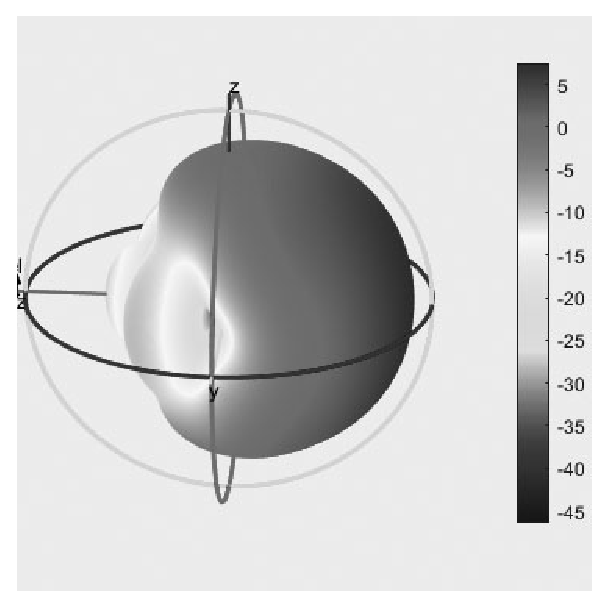
\includegraphics[width=\textwidth]{figs/wa5vjb_2_6G.eps}
\end{subfigure}
\hspace{\fill}
\begin{subfigure}[t]{0.22\textwidth}
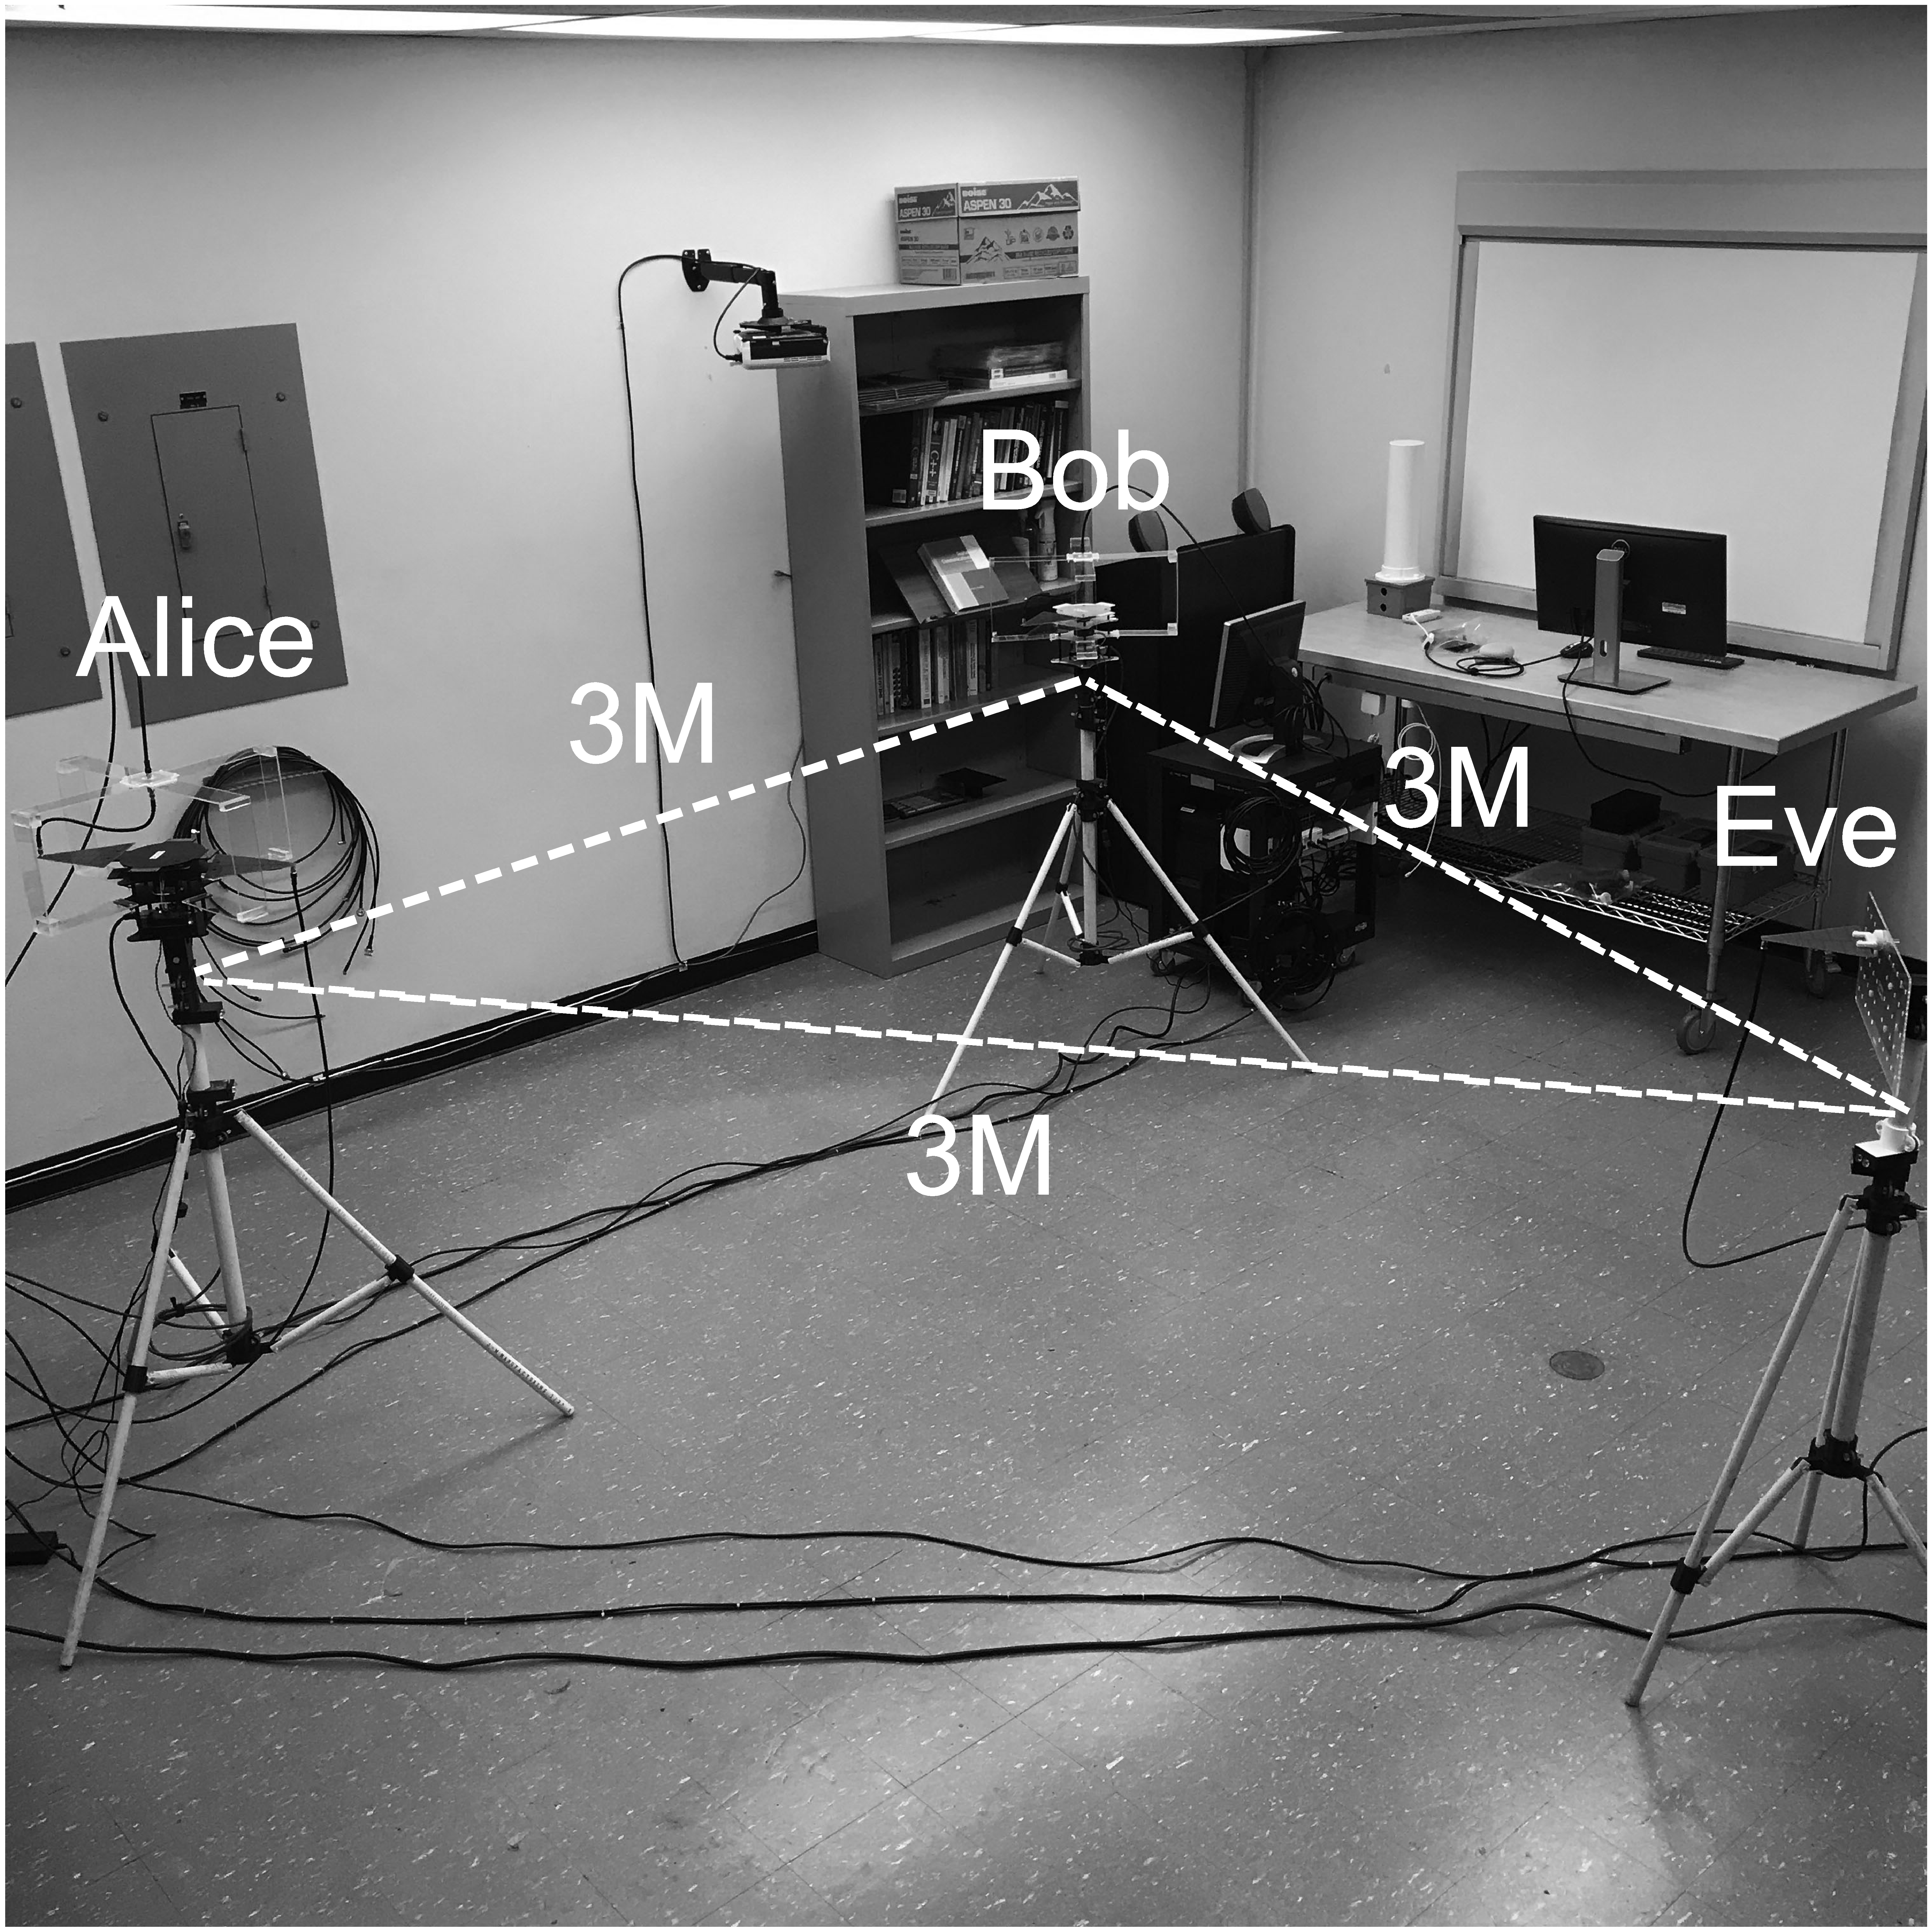
\includegraphics[width=\textwidth]{figs/IMG_1668.eps}
\end{subfigure}
\hspace{\fill}
\begin{subfigure}[t]{0.22\textwidth}
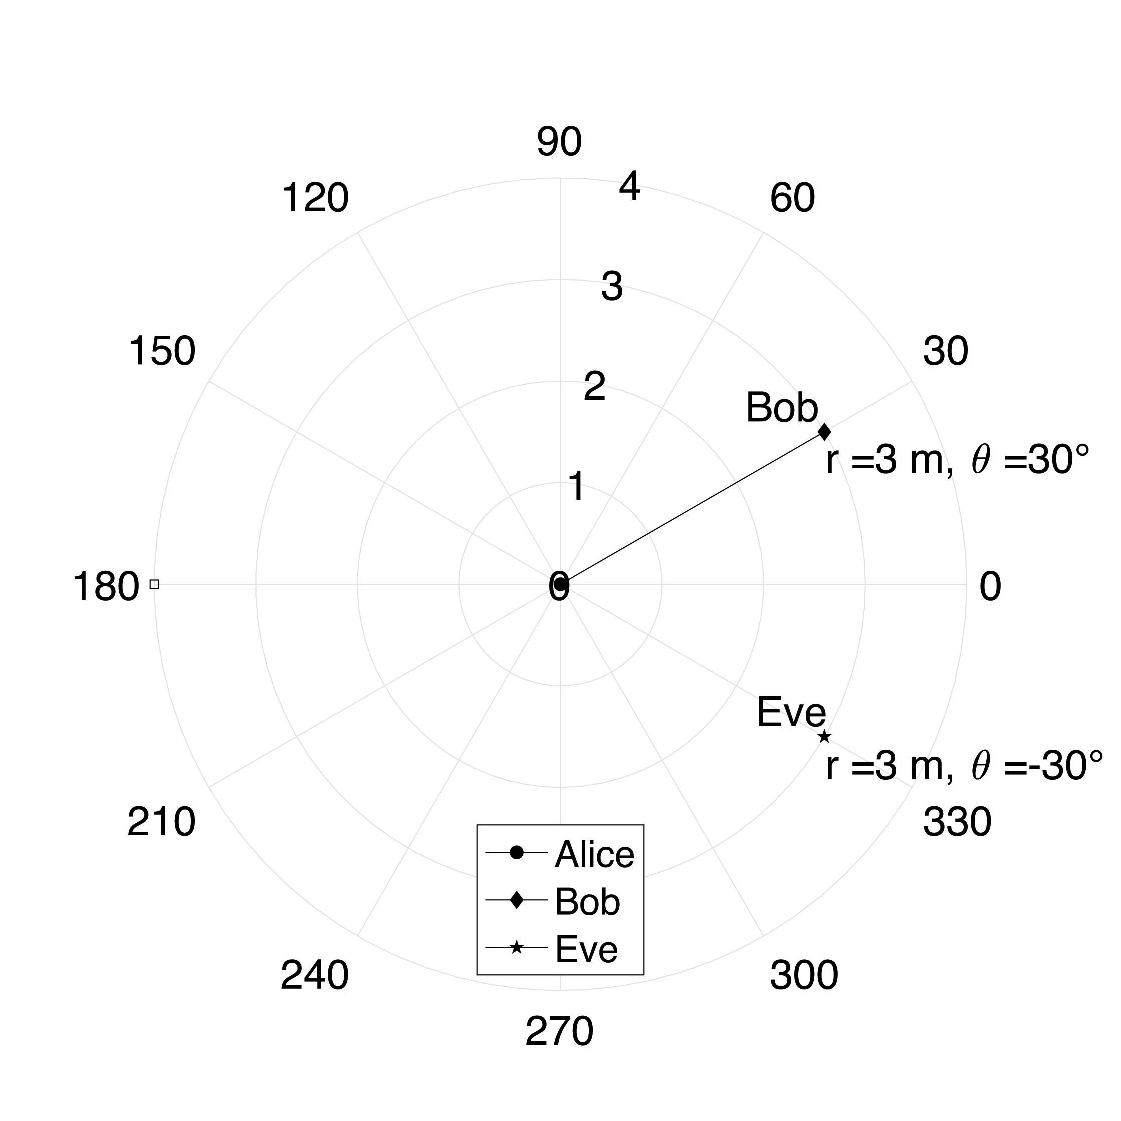
\includegraphics[width=\textwidth]{figs/plot.eps}
\end{subfigure}
\caption{From top to bottom, left to right: (a) SER of Bob and Eve over the number of training modes. SNR = 25dB; NDR = 1. (b) SER of Bob over Alice's NDR for different SNRs, with 20 training modes. (c) Eve's SER over the number of iterations; SNR = 25dB; various NDR. (d) Eve's SER over the number of iterations. NDR = 1; various SNR. (e) Eve's SER over the number of iterations; SNR = 25dB; NDR = 1; various antenna switching period. (f) Azimuth CSI magnitude distribution estimated with compressive
sensing algorithm. (g) SER of Bob and Eve over the number of training mode based on the real-world channel data. (h) Real-world rotator. (i) Radiation pattern of the RA. (j) Real-world experiment setup. (k) Geometry of the setup.}
\label{fig:performance}
\end{figure*}

In this section, we evaluate the performance of our  scheme under the practical known-plaintext attack with both simulation and real-world experiments. We start with the overview of simulation setup, and investigate the effects of various parameters. With simulation, we can cover a wide parameter range and establish the operating environment for the known-plaintext attack with a MIMO eavesdropper. Then with an implementation using USRP platform and a rotating RA, we validate the simulation results via experiments. 

\subsection{Customized Reconfigurable Antenna}
For the channel randomization purpose, we prefer RAs with distinct radiation patterns across different antenna modes. There are different types of RAs in the literature \cite{bernhard2007reconfigurable,LiBeamSteeringReconfigurableAntenna2015}, however, most of them are designed for communication purpose that only steer to several directions, which results in similar radiation patterns over antenna modes and makes them unsuitable for channel randomization purpose. To better evaluate our ROBin scheme, we build our own RA by rotating a log periodic antenna manufactured by Ettus Research \cite{antenna}. We first measure all the design parameters for the given log periodic antenna, including arm width, arm spacing and etc., then its radiation pattern is simulated using MALTAB antenna toolbox and illustrated in Fig. \ref{fig:performance}i. In the simulation, we rotate the antenna every one degree, so that we have 360 antennas modes in total. And in practice, the rotator is constructed with a motor and  a microcontroller, to rotate the antenna agilely to an arbitrary angle in the azimuth plane. The rotator is illustrated in Fig. \ref{fig:performance}h. Note that, we can have various antenna configurations at Alice's side when Alice has multiple antennas in general, e.g. Alice can enrich antenna patterns by varying the gain level of each antenna, which can be achieved with power allocation among RF chains. Also, Alice can have more antennas than use and randomly selects one among them for transmission, or randomize the power ratio among antennas to introduce additional randomness to wireless channels as in \cite{hassanieh2015securing}.

% Hassanieh et al. in  \cite{hassanieh2015securing} also constructed a similar platform by rotating the transmitter with a fan motor at a constant speed. The transmitter is equipped with eight antennas, and each time a micro-controller randomly activates an antenna for transmission. However, for an eavesdropper who is able to measure the CSI of possible paths, the constant speed rotation allows him/her to predict the positions of antennas. In this way, the attacker can brute force the corresponding CSI of eight antennas to decode the message. In contrast, we rotate with a random speed \textcolor{red}{not sure}


\subsection{Simulation Setup}
As described in the system model, Alice, Bob and Eve are multi-antenna users with OFDM transmitters. W.l.o.g, we focus our simulation on a setup where Alice has two given log periodic antennas, Bob and Eve have one and two omnidirectional antenna(sTFor data transmission, the 30MHz wide AWGN channel is split into 48 equally spaced sub-channels, and the OFDM frames contain 192 symbols for each sub-channel. To evaluate the effect of Alice's AN, we vary the ratio of AN to the transmitted data signal, namely that Noise to Data Ratio (NDR). With fixed transmit power, the power for data signal is:
\begin{equation}
    D = \frac{1}{\text{NDR}+1}\begin{pmatrix}
        D_B\\
        \text{NDR} \cdot \text{AN}
    \end{pmatrix} 
\end{equation}
We simulate 100 different environment settings, where five scatters are put for each of them and the data signal are transmitted as 4-QAM symbols. The distance from Eve to Bob is set as $150$cm, which is 12 times of the signal wavelength. For all the simulations, we consider a more practical eavesdropper than that in theoretical analysis, where not all the historical data signal are known to the eavesdropper. Then we define the switching period $T$ of RA based on an OFDM frame, and 120 frames are sent during the channel coherent time, hence we have $T \in [1,120]$. For each frame, the attacker is assumed to obtain two symbols. 
Then if $T = 10$, it means that the transmission mode changes every ten packets, hence for a given transmit filter (computed from the given transmission mode), the attacker has 20 known symbols for filter training.
% where the symbols known by attackers are from the well-known protocols in the WiFi frame. Though no pilots are needed in transmission phase of ROBin, the attacker is still able to guess parts of symbols from information like addresses. However, the attacker is not able to obtain all the historical data signal in practice. Besides, since AN is not intended for the receiver, it is random data in general, which makes it hard for the attacker to get enough plaintext and identify the  correct  decoding  filter. Correspondingly, we define the switching period $T$ of RA based on an OFDM frame, and 120 frames are sent during the channel coherent time, hence we have $T \in [1,120]$. For each frame, the attacker is assumed to obtain two symbols. 
% Then if $T = 10$, it means that the transmission mode changes every ten packets, hence for a given transmit filter (computed from the given transmission mode), the attacker has 20 known symbols for filter training.

% \begin{figure}[t]
%     \Large
%     \centering
%     \resizebox{0.5\columnwidth}{!}{% This file was created by matlab2tikz.
% Minimal pgfplots version: 1.3
%
%The latest updates can be retrieved from
%  http://www.mathworks.com/matlabcentral/fileexchange/22022-matlab2tikz
%where you can also make suggestions and rate matlab2tikz.
%
\begin{tikzpicture}

\begin{axis}[%
width=\tikzfigW,
height=\tikzfigH,
at={(0.758333in,0.525in)},
scale only axis,
xmin=10,
xmax=40,
xtick={10, 20, 30, 40},
xlabel={No. of training modes},
ymode=log,
ymin=1e-08,
ymax=1,
ytick={ 1e-08,  1e-06, 0.0001,   0.01,    0.1},
yminorticks=true,
ylabel={SER},
label style={font=\small},
tick label style={font=\small},
legend style={at={(0.45,0.4)},anchor=south west,legend cell align=left,align=left,draw=white!15!black,font=\scriptsize}
]
\addplot [color=black,solid,line width=1.0pt]
  table[row sep=crcr]{%
10	0.0187450086805556\\
20	0.00150703125\\
30	3.90624999999978e-07\\
40	4.34027777777778e-08\\
};
\addlegendentry{$\text{Bob}_{\text{ROBin}}$};

\addplot [color=black,solid,line width=1.0pt,mark=star,mark options={solid}]
  table[row sep=crcr]{%
10	0.0603373263888889\\
20	0.0673694444444444\\
30	0.0612369357638889\\
40	0.0602316840277778\\
};
\addlegendentry{$\text{Eve}_{\text{ROBin}}$};

\addplot [color=black,dash dot,line width=1.0pt]
  table[row sep=crcr]{%
10	4.34027777777778e-08\\
20	4.34027777777778e-08\\
30	4.34027777777778e-08\\
40	4.34027777777778e-08\\
};
\addlegendentry{$\text{Bob}$};

\addplot [color=black,dashed,line width=1.0pt]
  table[row sep=crcr]
%     \caption{SER of Bob and Eve over the number of training modes. SNR = 25dB; NDR = 1; Eve's SER is obtained after 240 iterations.}
%     \label{fig:numSamples}
% \end{figure}
% \begin{figure}[t]
%     \Large
%     \centering
%     \resizebox{0.5\columnwidth}{!}{% This file was created by matlab2tikz.
% Minimal pgfplots version: 1.3
%
%The latest updates can be retrieved from
%  http://www.mathworks.com/matlabcentral/fileexchange/22022-matlab2tikz
%where you can also make suggestions and rate matlab2tikz.
%
\begin{tikzpicture}

\begin{axis}[%
width=\tikzfigW,
height=\tikzfigH,
at={(0.758333in,0.490972in)},
scale only axis,
xmin=1,
xmax=10,
xtick={ 1,  2,  4,  6,  8, 10},
xlabel={NDR},
ymode=log,
ymin=1e-08,
ymax=1,
ytick={ 1e-08,  1e-06, 0.0001,   0.01,      1},
yminorticks=true,
ylabel={Bob's SER},
label style={font=\small},
tick label style={font=\small},
legend style={at={(0.25,0.04)},anchor=south west,legend cell align=left,align=left,draw=white!15!black,font=\scriptsize}
]
% \addplot [color=black,dashed,line width=1.0pt]
%   table[row sep=crcr]{%
% 1	0.000986111111111111\\
% 2	0.00493433159722222\\
% 4	0.0260634548611111\\
% 6	0.0590388454861111\\
% 8	0.0982852864583333\\
% 10	0.137298567708333\\
% };
% \addlegendentry{$\text{SNR}_{\text{ROBin}}\text{=15dB}$}

% \addplot [color=black,dashed,line width=1.0pt,mark=x,mark options={solid}]
%   table[row sep=crcr]{%
% 1	0.000128602430555556\\
% 2	0.00164865451388889\\
% 4	0.00938823784722223\\
% 6	0.0204099392361111\\
% 8	0.0361276041666667\\
% 10	0.0567549479166667\\
% };
% \addlegendentry{$\text{SNR}_{\text{ROBin}}\text{=20dB}$}

\addplot [color=black,solid,line width=1.0pt]
  table[row sep=crcr]{%
1	0.000122743055555556\\
2	0.00112291666666667\\
4	0.00599483506944444\\
6	0.0107560329861111\\
8	0.0175454427083333\\
10	0.0252785590277778\\
};
\addlegendentry{$\text{SNR}_{\text{ROBin}}\text{=25dB}$}

\addplot [color=black,dashed,line width=1.0pt]
  table[row sep=crcr]{%
1	6.77083333333328e-06\\
2	0.00128888888888889\\
4	0.00580078125\\
6	0.00843862847222222\\
8	0.012955859375\\
10	0.0177450954861111\\
};
\addlegendentry{$\text{SNR}_{\text{ROBin}}\text{=30dB}$}


% \addplot [color=black,solid,line width=1.0pt]
%   table[row sep=crcr]{%
% 1	0.000699652777777778\\
% 2	0.00341688368055556\\
% 4	0.0201337239583333\\
% 6	0.0510474826388889\\
% 8	0.0879983506944444\\
% 10	0.125694965277778\\
% };
% \addlegendentry{$\text{SNR}_\text{OB}\text{=15dB}$};

% \addplot [color=black,solid,line width=1.0pt,mark=x,mark options={solid}]
%   table[row sep=crcr]{%
% 1	4.60069444444446e-05\\
% 2	0.000383159722222222\\
% 4	0.00349991319444444\\
% 6	0.01133359375\\
% 8	0.0246471788194444\\
% 10	0.0419066840277778\\
% };
% \addlegendentry{$\text{SNR}_\text{OB}\text{=20dB}$};

\addplot [color=black,dash dot,line width=1.0pt]
  table[row sep=crcr]{%
1	8.68055555555136e-08\\
2	7.20486111111118e-06\\
4	0.000420486111111111\\
6	0.00194926215277778\\
8	0.00467591145833333\\
10	0.00904301215277778\\
};
\addlegendentry{$\text{SNR}_\text{OB}\text{=25dB}$};

\addplot [color=black,solid,line width=1.0pt,mark=star,mark options={solid}]
  table[row sep=crcr]
%     \caption{SER of Bob over Alice's NDR for differnetn SNRs. Number of training modes is 20.}
%     \label{fig:SNRNDR}
% \end{figure}

\subsection{Effect of the number of training modes}
Since the estimation of the AoD distribution is based on compressive sensing in ROBin, theoretically, the more training modes we use, the more precise the estimation will be. Fig. \ref{fig:performance}a illustrates the SER of Bob and Eve over the number of training modes, obtained under ROBin and orthogonal blinding. Here to better show the impact of channel prediction to Bob's SER, we do not change the antenna mode during transmission, which is to set $T = 120$, then the only difference of these two schemes is that ROBin computes the transmit filter based on the predicted channel, while orthogonal blinding uses the measured channel matrix obtained from channel sounding. 
% With log scale, when SER is 0, we substitute it with the SER that only one symbol is incorrectly demodulated over all the experiments, which is $4.34 \times 10^{-8}$ in this case. 
From Fig. \ref{fig:performance}a we can see that there is a gap between Bob's SER obtained from two schemes, which is caused by the imperfect channel prediction and the missing channel sounding. However, it decreases with the number of training modes as expected, and when 20 training modes are used, Bob's SER is small enough for communication. On the other hand, Eve's SER obtained after 240 iterations is quite stable under the different number of training modes, this is because the effect of the transmit filter and artificial noise are both filtered out by Eve's receive filter.

\subsection{Effect of artificial noise and channel noise to Bob}
Fig. \ref{fig:performance}b shows Bob's SER with orthogonal blinding and ROBin, at this time the antenna switching period is set as $T = 6$, hence 20 transmission modes are used under a given environmental setting. From Fig. \ref{fig:performance}b, we can see that Bob's SER decreases as SNR increases under both schemes. Especially, both SNR and NDR have significant impacts on Bob's SER for orthogonal blinding. In contrast, the increase of SNR does not bring much benefit to Bob's SER for ROBin, since Bob's SER is dominated by the precise of channel prediction. Due to the imperfect channel prediction, part of the artificial noise is leaked to Bob's channel, which increases Bob's SER. Fortunately, as long as the NDR is not too large, the communication quality is still guaranteed. For instance, when SNR = 25dB and NDR = 2, Bob can still achieve an average SER of $1.1 \times 10^{-3}$. 

\subsection{Effect of artificial noise and channel noise to Eve}
Theoretically, the higher the NDR is, the higher is the SER on Eve's side. Here we set the antenna switching period as $T = 60$ to provide Eve some advantages. In Fig. \ref{fig:performance}c, we illustrate how Alice's NDR affects Eve's performance. As we expected, Eve's SER decreases with the increase of NDR. It is worth noticing that, when the power of artificial noise is not too strong, $\text{NDR} \leq 4$ for instance, we can see that Eve's SER has an obvious reduction with the iterative process; whereas, as the artificial noise becomes stronger, even if the number of iterations increases, the decrease of Eve's SER is not significant. 
Besides, in Fig. \ref{fig:performance}d we illustrate how SNR affects Eve's SER. The effect of channel noise to Eve's SER is much weaker than that to Bob's SER, no significant variation for Eve's SER with the increase of SNR. Hence we can conclude that Eve's attack performance is mainly constrained by the power of artificial noise that Alice sent. And there is a tradeoff between the system secrecy (Eve's SER) and the communication quality (Bob's SER) when injecting artificial noise to the channel.

% \begin{figure}[t]
%     \Large
%     \centering
%     \resizebox{0.5\columnwidth}{!}{% This file was created by matlab2tikz.
% Minimal pgfplots version: 1.3
%
%The latest updates can be retrieved from
%  http://www.mathworks.com/matlabcentral/fileexchange/22022-matlab2tikz
%where you can also make suggestions and rate matlab2tikz.
%
\begin{tikzpicture}

\begin{axis}[%
width=\tikzfigW,
height=\tikzfigH,
%at={(0.758333in,0.490972in)},
scale only axis,
xmin=0,
xmax=250,
xlabel={Number of Iterations},
ymin=0.35,
ymax=0.75,
xtick={ 0, 50, 100, 150, 200, 250},
ytick={ 0.3, 0.45, 0.55, 0.65, 0.75},
ylabel={Eve's SER},
label style={font=\small},
tick label style={font=\small},
legend style={at={(0.4,0.35)},anchor=south west,legend cell align=left,align=left,draw=white!15!black,font=\scriptsize}
]
\addplot [color=black,double,line width=1.0pt]
  table[row sep=crcr]{%
1	0.714592881944445\\
2	0.674533854166667\\
3	0.646288194444445\\
4	0.639197048611111\\
5	0.608267795138889\\
6	0.591979166666667\\
7	0.577979166666667\\
8	0.56727734375\\
9	0.55693359375\\
10	0.548439236111111\\
11	0.53977734375\\
12	0.533875\\
13	0.526740885416667\\
14	0.523\\
15	0.517506944444444\\
16	0.508233940972222\\
17	0.498724826388889\\
18	0.493434461805556\\
19	0.491013020833333\\
20	0.487888020833333\\
21	0.483762152777778\\
22	0.483190104166667\\
23	0.481740885416667\\
24	0.47898828125\\
25	0.47512890625\\
26	0.471596354166667\\
27	0.466875434027778\\
28	0.462352864583333\\
29	0.461723958333333\\
30	0.461149305555555\\
31	0.460009548611111\\
32	0.457713541666667\\
33	0.457713541666667\\
34	0.457713541666667\\
35	0.455958767361111\\
36	0.454307291666667\\
37	0.45384375\\
38	0.453666232638889\\
39	0.449940538194444\\
40	0.449754774305556\\
41	0.447524305555556\\
42	0.446190538194444\\
43	0.446190538194444\\
44	0.4450234375\\
45	0.444446614583333\\
46	0.442932725694444\\
47	0.440263020833333\\
48	0.440263020833333\\
49	0.439627604166667\\
50	0.439627604166667\\
51	0.438510850694445\\
52	0.436240017361111\\
53	0.434579427083333\\
54	0.433573784722222\\
55	0.432697916666667\\
56	0.430939236111111\\
57	0.430607638888889\\
58	0.428844184027778\\
59	0.428799479166667\\
60	0.428799479166667\\
61	0.426791232638889\\
62	0.426525173611111\\
63	0.426102430555556\\
64	0.425759982638889\\
65	0.425759982638889\\
66	0.425759982638889\\
67	0.425759982638889\\
68	0.423932725694444\\
69	0.422850694444444\\
70	0.422567274305556\\
71	0.422567274305556\\
72	0.422539930555556\\
73	0.420638020833333\\
74	0.420637152777778\\
75	0.420635416666667\\
76	0.420328993055556\\
77	0.420328993055556\\
78	0.420328993055556\\
79	0.419638020833333\\
80	0.419638020833333\\
81	0.419092013888889\\
82	0.419075954861111\\
83	0.418581597222222\\
84	0.418415798611111\\
85	0.415895833333333\\
86	0.415387586805556\\
87	0.415358072916667\\
88	0.415009114583333\\
89	0.414886284722222\\
90	0.414879340277778\\
91	0.4145078125\\
92	0.414423177083333\\
93	0.414423177083333\\
94	0.414386284722222\\
95	0.414386284722222\\
96	0.414385850694444\\
97	0.414357638888889\\
98	0.414334201388889\\
99	0.414026041666667\\
100	0.414026041666667\\
101	0.413739149305556\\
102	0.413739149305556\\
103	0.413342013888889\\
104	0.413342013888889\\
105	0.413342013888889\\
106	0.412254340277778\\
107	0.412254340277778\\
108	0.412254340277778\\
109	0.412254340277778\\
110	0.412254340277778\\
111	0.412081597222222\\
112	0.412081163194444\\
113	0.412061631944444\\
114	0.41101171875\\
115	0.41101171875\\
116	0.410981770833333\\
117	0.409819444444444\\
118	0.409817274305556\\
119	0.409817274305556\\
120	0.409817274305556\\
121	0.409817274305556\\
122	0.409806857638889\\
123	0.409806857638889\\
124	0.409806857638889\\
125	0.409490451388889\\
126	0.409490451388889\\
127	0.409490451388889\\
128	0.408853732638889\\
129	0.408853732638889\\
130	0.408851996527778\\
131	0.408851996527778\\
132	0.408851996527778\\
133	0.408654947916667\\
134	0.408654947916667\\
135	0.408654947916667\\
136	0.40758984375\\
137	0.40758984375\\
138	0.407583767361111\\
139	0.407583767361111\\
140	0.407583767361111\\
141	0.407583767361111\\
142	0.407583767361111\\
143	0.407548611111111\\
144	0.407548611111111\\
145	0.407548611111111\\
146	0.407014322916667\\
147	0.407014322916667\\
148	0.407014322916667\\
149	0.407014322916667\\
150	0.407014322916667\\
151	0.406959635416667\\
152	0.406959635416667\\
153	0.406959635416667\\
154	0.406959635416667\\
155	0.406655381944445\\
156	0.406655381944445\\
157	0.406655381944445\\
158	0.406655381944445\\
159	0.406655381944445\\
160	0.406655381944445\\
161	0.406655381944445\\
162	0.406655381944445\\
163	0.4064921875\\
164	0.405970920138889\\
165	0.405970920138889\\
166	0.405970920138889\\
167	0.405970920138889\\
168	0.405970920138889\\
169	0.405970920138889\\
170	0.405970920138889\\
171	0.405970920138889\\
172	0.405957899305556\\
173	0.405930121527778\\
174	0.405930121527778\\
175	0.405930121527778\\
176	0.405930121527778\\
177	0.405930121527778\\
178	0.405605034722222\\
179	0.405604600694445\\
180	0.405604600694445\\
181	0.405604600694445\\
182	0.4055390625\\
183	0.405524305555556\\
184	0.405515625\\
185	0.405434461805556\\
186	0.405434461805556\\
187	0.405434461805556\\
188	0.405434027777778\\
189	0.405434027777778\\
190	0.405434027777778\\
191	0.405433159722222\\
192	0.405433159722222\\
193	0.405433159722222\\
194	0.405433159722222\\
195	0.405433159722222\\
196	0.405433159722222\\
197	0.405433159722222\\
198	0.405433159722222\\
199	0.405426215277778\\
200	0.404825086805556\\
201	0.404825086805556\\
202	0.404805555555556\\
203	0.404805555555556\\
204	0.403477864583333\\
205	0.403222222222222\\
206	0.403222222222222\\
207	0.403222222222222\\
208	0.401485677083333\\
209	0.401485677083333\\
210	0.401485677083333\\
211	0.40121875\\
212	0.40121875\\
213	0.40121875\\
214	0.40121875\\
215	0.40121875\\
216	0.40121875\\
217	0.40121875\\
218	0.401112847222222\\
219	0.401112847222222\\
220	0.401112847222222\\
221	0.401112847222222\\
222	0.400892795138889\\
223	0.400832465277778\\
224	0.400832465277778\\
225	0.400335503472222\\
226	0.400335503472222\\
227	0.400335503472222\\
228	0.400335503472222\\
229	0.400335503472222\\
230	0.400217447916667\\
231	0.400217447916667\\
232	0.400217447916667\\
233	0.400128472222222\\
234	0.400128472222222\\
235	0.399789496527778\\
236	0.399789496527778\\
237	0.399514756944445\\
238	0.399514756944445\\
239	0.399514756944445\\
240	0.399514756944445\\
};
\addlegendentry{NDR=1};

\addplot [color=black,dash dot,line width=1.0pt]
  table[row sep=crcr]{%
1	0.710848090277778\\
2	0.698789930555556\\
3	0.680871961805556\\
4	0.674679253472222\\
5	0.6576796875\\
6	0.648643663194445\\
7	0.641080729166667\\
8	0.637694010416667\\
9	0.631934461805556\\
10	0.626782552083333\\
11	0.621791232638889\\
12	0.618710503472222\\
13	0.616751736111111\\
14	0.612813802083333\\
15	0.608802951388889\\
16	0.608465711805556\\
17	0.605220486111111\\
18	0.602271701388889\\
19	0.596276475694445\\
20	0.59311328125\\
21	0.591311197916666\\
22	0.584938368055555\\
23	0.583009982638889\\
24	0.5816796875\\
25	0.577289496527778\\
26	0.576146701388889\\
27	0.572860677083333\\
28	0.570184895833334\\
29	0.568718315972222\\
30	0.564602864583334\\
31	0.563834201388889\\
32	0.56230859375\\
33	0.558663628472222\\
34	0.557739149305556\\
35	0.556705295138889\\
36	0.554381510416667\\
37	0.554180121527778\\
38	0.552649739583333\\
39	0.550235677083333\\
40	0.548788194444444\\
41	0.548545572916667\\
42	0.546330295138889\\
43	0.543867621527778\\
44	0.542759114583333\\
45	0.540443142361111\\
46	0.5403515625\\
47	0.537802083333333\\
48	0.537756076388889\\
49	0.536391059027778\\
50	0.535287760416667\\
51	0.533506944444445\\
52	0.532684461805556\\
53	0.530159722222222\\
54	0.529042534722222\\
55	0.5289140625\\
56	0.527090277777778\\
57	0.524095052083334\\
58	0.518552951388889\\
59	0.518362413194444\\
60	0.518057291666667\\
61	0.51770703125\\
62	0.516913194444445\\
63	0.516312934027778\\
64	0.516047743055556\\
65	0.514745659722222\\
66	0.514745659722222\\
67	0.512763888888889\\
68	0.512760416666667\\
69	0.512582465277778\\
70	0.512582465277778\\
71	0.51222265625\\
72	0.512204861111111\\
73	0.508993923611111\\
74	0.508806857638889\\
75	0.508566840277778\\
76	0.508377604166667\\
77	0.508377604166667\\
78	0.508375\\
79	0.50833203125\\
80	0.506624565972222\\
81	0.50651171875\\
82	0.50611328125\\
83	0.5057265625\\
84	0.505297743055556\\
85	0.503138454861111\\
86	0.503116319444444\\
87	0.501066840277778\\
88	0.4990625\\
89	0.496736979166667\\
90	0.496636284722222\\
91	0.496633680555555\\
92	0.496592447916667\\
93	0.496578559027778\\
94	0.496368923611111\\
95	0.495852864583333\\
96	0.495852864583333\\
97	0.495456163194444\\
98	0.493940104166667\\
99	0.493789496527778\\
100	0.4929765625\\
101	0.491664496527778\\
102	0.488654513888889\\
103	0.487847222222222\\
104	0.487847222222222\\
105	0.487825520833333\\
106	0.487789930555556\\
107	0.486236979166667\\
108	0.486236979166667\\
109	0.486223090277778\\
110	0.486039930555556\\
111	0.485891493055556\\
112	0.484575954861111\\
113	0.484505208333333\\
114	0.484505208333333\\
115	0.484189236111111\\
116	0.4836875\\
117	0.483649305555556\\
118	0.482748263888889\\
119	0.482662760416667\\
120	0.48226953125\\
121	0.482002170138889\\
122	0.481973958333333\\
123	0.481973958333333\\
124	0.481973958333333\\
125	0.48144921875\\
126	0.48144921875\\
127	0.481420138888889\\
128	0.480919270833333\\
129	0.48085546875\\
130	0.48085546875\\
131	0.480456597222222\\
132	0.48036328125\\
133	0.479254340277778\\
134	0.479205295138889\\
135	0.479174913194444\\
136	0.47916796875\\
137	0.479085069444444\\
138	0.47892578125\\
139	0.478852864583333\\
140	0.477772569444444\\
141	0.477772569444444\\
142	0.477772569444444\\
143	0.477384548611111\\
144	0.477097222222222\\
145	0.477021267361111\\
146	0.477021267361111\\
147	0.477021267361111\\
148	0.477020399305556\\
149	0.476991753472222\\
150	0.476991753472222\\
151	0.476991753472222\\
152	0.476962673611111\\
153	0.476634548611111\\
154	0.476634548611111\\
155	0.476611979166667\\
156	0.476478732638889\\
157	0.476307725694444\\
158	0.475995659722222\\
159	0.475946180555556\\
160	0.475900607638889\\
161	0.475318142361111\\
162	0.475270399305556\\
163	0.475270399305556\\
164	0.475270399305556\\
165	0.47519921875\\
166	0.474144965277778\\
167	0.473908854166667\\
168	0.473546006944444\\
169	0.473546006944444\\
170	0.473546006944444\\
171	0.473546006944444\\
172	0.473546006944444\\
173	0.473492621527778\\
174	0.473492621527778\\
175	0.473465711805556\\
176	0.473465711805556\\
177	0.473465711805556\\
178	0.473365885416667\\
179	0.473330295138889\\
180	0.473325954861111\\
181	0.473325954861111\\
182	0.473254774305556\\
183	0.473241319444444\\
184	0.473241319444444\\
185	0.473241319444444\\
186	0.473241319444444\\
187	0.473241319444444\\
188	0.473172743055556\\
189	0.472678819444444\\
190	0.472650607638889\\
191	0.472589409722222\\
192	0.471187065972222\\
193	0.471187065972222\\
194	0.469980034722222\\
195	0.469980034722222\\
196	0.468310763888889\\
197	0.468310763888889\\
198	0.468310763888889\\
199	0.468310763888889\\
200	0.468148871527778\\
201	0.467302951388889\\
202	0.465709201388889\\
203	0.465709201388889\\
204	0.465509548611111\\
205	0.465509548611111\\
206	0.465247395833333\\
207	0.465247395833333\\
208	0.465157118055556\\
209	0.465157118055556\\
210	0.465157118055556\\
211	0.463236979166667\\
212	0.463236979166667\\
213	0.463236979166667\\
214	0.463236979166667\\
215	0.463236979166667\\
216	0.463187065972222\\
217	0.463187065972222\\
218	0.463187065972222\\
219	0.463187065972222\\
220	0.463187065972222\\
221	0.462751736111111\\
222	0.462751736111111\\
223	0.462751736111111\\
224	0.462676649305556\\
225	0.462676649305556\\
226	0.462676649305556\\
227	0.462676649305556\\
228	0.462676649305556\\
229	0.462671440972222\\
230	0.461669270833333\\
231	0.461641059027778\\
232	0.461634114583333\\
233	0.461567708333333\\
234	0.461540798611111\\
235	0.461266059027778\\
236	0.461067708333333\\
237	0.460955295138889\\
238	0.460940538194444\\
239	0.460921006944444\\
240	0.460921006944444\\
};
\addlegendentry{NDR=2};

\addplot [color=black,dash pattern={on 7pt off 2pt on 1pt off 3pt},line width=1.0pt]
  table[row sep=crcr]{%
1	0.727302517361111\\
2	0.717838541666667\\
3	0.712375434027778\\
4	0.703504774305556\\
5	0.690833333333333\\
6	0.687000868055555\\
7	0.678313368055555\\
8	0.672259114583333\\
9	0.667538628472222\\
10	0.663371527777778\\
11	0.661121527777778\\
12	0.659459201388889\\
13	0.657967447916667\\
14	0.655009114583333\\
15	0.65425\\
16	0.649024305555556\\
17	0.646826822916667\\
18	0.646671875\\
19	0.645590277777778\\
20	0.637484375\\
21	0.635936197916667\\
22	0.633610243055556\\
23	0.631505208333333\\
24	0.630106336805556\\
25	0.625784722222222\\
26	0.62483203125\\
27	0.623167534722222\\
28	0.616668402777778\\
29	0.615658854166667\\
30	0.614338975694445\\
31	0.61403125\\
32	0.6125703125\\
33	0.61173046875\\
34	0.6108125\\
35	0.608401475694444\\
36	0.608161458333333\\
37	0.603966145833333\\
38	0.603391493055555\\
39	0.602495659722222\\
40	0.600479166666667\\
41	0.599174913194444\\
42	0.59638671875\\
43	0.59628125\\
44	0.589677951388889\\
45	0.584988715277778\\
46	0.582837673611111\\
47	0.582401475694444\\
48	0.581598958333333\\
49	0.578947482638889\\
50	0.578267361111111\\
51	0.57659765625\\
52	0.573326822916667\\
53	0.572567274305556\\
54	0.572029079861111\\
55	0.569092447916667\\
56	0.568534722222222\\
57	0.568521701388889\\
58	0.567871527777778\\
59	0.567065972222222\\
60	0.5662421875\\
61	0.565704861111111\\
62	0.564117621527778\\
63	0.564001736111111\\
64	0.561648003472222\\
65	0.561225694444444\\
66	0.561101128472222\\
67	0.560822916666667\\
68	0.559851996527778\\
69	0.558896701388889\\
70	0.557799913194444\\
71	0.554766927083333\\
72	0.554612847222222\\
73	0.5545078125\\
74	0.552812065972222\\
75	0.551641927083333\\
76	0.551446614583333\\
77	0.551417100694444\\
78	0.550857638888889\\
79	0.54856640625\\
80	0.548552517361111\\
81	0.548552517361111\\
82	0.548415798611111\\
83	0.547518663194444\\
84	0.547320746527778\\
85	0.5456015625\\
86	0.544114583333333\\
87	0.543718315972222\\
88	0.543718315972222\\
89	0.543384982638889\\
90	0.543354166666667\\
91	0.543354166666667\\
92	0.542685329861111\\
93	0.542291232638889\\
94	0.542291232638889\\
95	0.541704427083333\\
96	0.541392361111111\\
97	0.541184461805555\\
98	0.541184461805555\\
99	0.540395399305555\\
100	0.539813802083333\\
101	0.538690538194444\\
102	0.538312065972222\\
103	0.538296006944444\\
104	0.537884114583333\\
105	0.537766927083333\\
106	0.536621961805556\\
107	0.536621961805556\\
108	0.535848524305556\\
109	0.535439236111111\\
110	0.535439236111111\\
111	0.535439236111111\\
112	0.535287760416667\\
113	0.534663628472222\\
114	0.534647135416667\\
115	0.534647135416667\\
116	0.530291232638889\\
117	0.530080295138889\\
118	0.530080295138889\\
119	0.529895399305556\\
120	0.529838975694444\\
121	0.529279513888889\\
122	0.526983506944444\\
123	0.526917534722222\\
124	0.526810329861111\\
125	0.526668402777778\\
126	0.52662109375\\
127	0.52662109375\\
128	0.526598958333333\\
129	0.526335069444444\\
130	0.524943576388889\\
131	0.524927083333333\\
132	0.522205295138889\\
133	0.522193142361111\\
134	0.522189670138889\\
135	0.522157118055556\\
136	0.522115451388889\\
137	0.52210546875\\
138	0.521940972222222\\
139	0.521859375\\
140	0.521859375\\
141	0.521591145833333\\
142	0.521331163194445\\
143	0.52125390625\\
144	0.521032552083333\\
145	0.5204375\\
146	0.5204375\\
147	0.5204375\\
148	0.520275173611111\\
149	0.520275173611111\\
150	0.520200086805555\\
151	0.519489149305556\\
152	0.519065104166667\\
153	0.518360677083333\\
154	0.517512152777778\\
155	0.517458767361111\\
156	0.517458767361111\\
157	0.515874131944444\\
158	0.515450954861111\\
159	0.515450954861111\\
160	0.515384114583333\\
161	0.514747829861111\\
162	0.514663628472222\\
163	0.514663628472222\\
164	0.514640625\\
165	0.512838541666666\\
166	0.512815104166667\\
167	0.512815104166667\\
168	0.512815104166667\\
169	0.512815104166667\\
170	0.51209765625\\
171	0.51209375\\
172	0.51209375\\
173	0.51209375\\
174	0.51209375\\
175	0.512090711805555\\
176	0.511500868055555\\
177	0.511500868055555\\
178	0.511500868055555\\
179	0.511287326388889\\
180	0.510775607638889\\
181	0.510770833333333\\
182	0.510721788194444\\
183	0.510721788194444\\
184	0.510721788194444\\
185	0.510717881944444\\
186	0.510717881944444\\
187	0.510459201388889\\
188	0.510415364583333\\
189	0.510415364583333\\
190	0.510415364583333\\
191	0.510415364583333\\
192	0.510125\\
193	0.510097222222222\\
194	0.509569010416667\\
195	0.509569010416667\\
196	0.509518229166667\\
197	0.509512586805555\\
198	0.509506944444444\\
199	0.5086640625\\
200	0.50855859375\\
201	0.50786328125\\
202	0.507458333333333\\
203	0.507431423611111\\
204	0.507389322916666\\
205	0.507389322916666\\
206	0.507325086805555\\
207	0.5070546875\\
208	0.506970486111111\\
209	0.506571614583333\\
210	0.506052083333333\\
211	0.504655381944444\\
212	0.504522569444444\\
213	0.50358984375\\
214	0.50358984375\\
215	0.503589409722222\\
216	0.503589409722222\\
217	0.503588107638889\\
218	0.503588107638889\\
219	0.503583767361111\\
220	0.503578993055555\\
221	0.503578993055555\\
222	0.503560329861111\\
223	0.502473958333333\\
224	0.502458333333333\\
225	0.502194444444444\\
226	0.502153211805555\\
227	0.50213671875\\
228	0.50213671875\\
229	0.50213671875\\
230	0.501815538194444\\
231	0.500952256944444\\
232	0.500507378472222\\
233	0.500442708333333\\
234	0.500143663194444\\
235	0.500017795138889\\
236	0.49970703125\\
237	0.49793359375\\
238	0.497933159722222\\
239	0.497930121527778\\
240	0.497930121527778\\
};
\addlegendentry{NDR=4};

\addplot [color=black,densely dotted,line width=1.0pt]
  table[row sep=crcr]{%
1	0.736930989583333\\
2	0.728983940972222\\
3	0.723530815972222\\
4	0.720104166666667\\
5	0.716226996527778\\
6	0.713896267361111\\
7	0.712138020833333\\
8	0.704926215277778\\
9	0.699486545138889\\
10	0.697551215277778\\
11	0.694807291666666\\
12	0.693529947916667\\
13	0.690208333333333\\
14	0.687263888888889\\
15	0.685411458333333\\
16	0.684779079861111\\
17	0.682164930555556\\
18	0.679131076388889\\
19	0.678393229166667\\
20	0.6758828125\\
21	0.673772135416667\\
22	0.672923611111112\\
23	0.6727109375\\
24	0.671750868055556\\
25	0.669661024305556\\
26	0.666180121527778\\
27	0.664237847222222\\
28	0.663129340277778\\
29	0.662530381944444\\
30	0.661309461805555\\
31	0.660493489583333\\
32	0.660220052083333\\
33	0.659557291666666\\
34	0.657739583333333\\
35	0.656013888888889\\
36	0.655823350694445\\
37	0.655260850694445\\
38	0.654377170138889\\
39	0.653657118055556\\
40	0.651805555555556\\
41	0.651198784722222\\
42	0.650660590277778\\
43	0.649016927083333\\
44	0.645327256944444\\
45	0.645079861111111\\
46	0.644048611111111\\
47	0.643659722222222\\
48	0.640967013888889\\
49	0.640625\\
50	0.640592013888889\\
51	0.640111979166667\\
52	0.637448350694444\\
53	0.636641927083333\\
54	0.634262586805556\\
55	0.633559461805556\\
56	0.633421440972222\\
57	0.631158420138889\\
58	0.63016796875\\
59	0.628975260416667\\
60	0.627401909722222\\
61	0.626649305555556\\
62	0.626282118055556\\
63	0.624681423611111\\
64	0.622250868055556\\
65	0.621908854166667\\
66	0.621835503472222\\
67	0.6186171875\\
68	0.617512586805556\\
69	0.615838107638889\\
70	0.61534765625\\
71	0.615336371527778\\
72	0.610211805555556\\
73	0.60933984375\\
74	0.608960069444444\\
75	0.607020399305556\\
76	0.606733940972222\\
77	0.606642795138889\\
78	0.606224826388889\\
79	0.605553385416667\\
80	0.6054921875\\
81	0.605241319444445\\
82	0.604983940972223\\
83	0.604503038194445\\
84	0.603669704861111\\
85	0.601791666666667\\
86	0.601357204861111\\
87	0.601135416666667\\
88	0.59839453125\\
89	0.598305989583333\\
90	0.598043836805556\\
91	0.598030815972222\\
92	0.597171006944444\\
93	0.596659288194445\\
94	0.595907118055556\\
95	0.595745659722222\\
96	0.595167534722222\\
97	0.593523003472222\\
98	0.593497829861111\\
99	0.592659722222222\\
100	0.591790364583333\\
101	0.591685763888889\\
102	0.591673177083333\\
103	0.59015625\\
104	0.588774739583333\\
105	0.588773871527778\\
106	0.588184027777778\\
107	0.588122395833333\\
108	0.58812109375\\
109	0.588116319444445\\
110	0.587736979166667\\
111	0.585869357638889\\
112	0.5858359375\\
113	0.585830729166667\\
114	0.5836328125\\
115	0.5836328125\\
116	0.583611111111111\\
117	0.583171440972222\\
118	0.582507378472222\\
119	0.582262586805556\\
120	0.582253472222222\\
121	0.582159288194445\\
122	0.579944010416667\\
123	0.579769965277778\\
124	0.579722222222222\\
125	0.579486545138889\\
126	0.579352430555556\\
127	0.578797309027778\\
128	0.578787326388889\\
129	0.578787326388889\\
130	0.578643229166667\\
131	0.577865017361111\\
132	0.577841579861111\\
133	0.577841579861111\\
134	0.577628038194444\\
135	0.577585069444444\\
136	0.577581163194444\\
137	0.577580729166667\\
138	0.577576388888889\\
139	0.577576388888889\\
140	0.577573784722222\\
141	0.577569878472222\\
142	0.577555989583333\\
143	0.576946614583333\\
144	0.576946614583333\\
145	0.576946614583333\\
146	0.576340277777778\\
147	0.576272569444444\\
148	0.576269965277778\\
149	0.576248697916667\\
150	0.575739583333333\\
151	0.575739149305555\\
152	0.575707899305555\\
153	0.575705729166667\\
154	0.574211805555555\\
155	0.573995659722222\\
156	0.573987847222222\\
157	0.573987847222222\\
158	0.573811197916667\\
159	0.573811197916667\\
160	0.570755208333333\\
161	0.570755208333333\\
162	0.570732204861111\\
163	0.570732204861111\\
164	0.570732204861111\\
165	0.570684895833333\\
166	0.570643663194444\\
167	0.570643663194444\\
168	0.570578125\\
169	0.570572048611111\\
170	0.570572048611111\\
171	0.570559027777778\\
172	0.570529947916667\\
173	0.570424045138889\\
174	0.570418836805555\\
175	0.570303385416666\\
176	0.569407552083333\\
177	0.569407552083333\\
178	0.569407552083333\\
179	0.569361979166667\\
180	0.569361979166667\\
181	0.569360677083333\\
182	0.569336371527778\\
183	0.569336371527778\\
184	0.569328993055555\\
185	0.568865017361111\\
186	0.568865017361111\\
187	0.56855078125\\
188	0.568469184027778\\
189	0.568283854166667\\
190	0.568283854166667\\
191	0.568262586805556\\
192	0.568192274305555\\
193	0.568192274305555\\
194	0.5681875\\
195	0.568151475694444\\
196	0.568142795138889\\
197	0.568142795138889\\
198	0.567983072916667\\
199	0.567983072916667\\
200	0.5677890625\\
201	0.566731770833333\\
202	0.566731770833333\\
203	0.566543402777778\\
204	0.566065538194444\\
205	0.565783854166667\\
206	0.565717013888889\\
207	0.564253038194444\\
208	0.564222222222222\\
209	0.564222222222222\\
210	0.564082899305556\\
211	0.563896701388889\\
212	0.563821614583333\\
213	0.563821614583333\\
214	0.5634609375\\
215	0.562989583333333\\
216	0.562930555555555\\
217	0.562923611111111\\
218	0.562846354166667\\
219	0.562805555555555\\
220	0.561975694444445\\
221	0.561965277777778\\
222	0.561961805555556\\
223	0.561725694444444\\
224	0.561723958333333\\
225	0.561670572916667\\
226	0.561654079861111\\
227	0.561641059027778\\
228	0.561590711805556\\
229	0.561559461805556\\
230	0.560691840277778\\
231	0.560328993055556\\
232	0.560039930555555\\
233	0.559977430555555\\
234	0.559977430555555\\
235	0.559133680555556\\
236	0.559133680555556\\
237	0.558647135416667\\
238	0.558647135416667\\
239	0.558646267361111\\
240	0.558646267361111\\
};
\addlegendentry{NDR=6};

\addplot [color=black,solid,line width=1.0pt]
  table[row sep=crcr]{%
1	0.740141927083333\\
2	0.733133246527778\\
3	0.72987109375\\
4	0.727395399305556\\
5	0.719627604166667\\
6	0.717170138888889\\
7	0.716337673611111\\
8	0.709243923611111\\
9	0.706088107638889\\
10	0.705337239583333\\
11	0.701192708333333\\
12	0.697536024305556\\
13	0.69621875\\
14	0.695335503472222\\
15	0.694673611111111\\
16	0.693897135416667\\
17	0.693206597222222\\
18	0.691590277777778\\
19	0.688572048611111\\
20	0.686924479166667\\
21	0.68527734375\\
22	0.682381510416667\\
23	0.680674045138889\\
24	0.680411892361111\\
25	0.679916666666667\\
26	0.678376302083334\\
27	0.676076388888889\\
28	0.674529513888889\\
29	0.672571180555556\\
30	0.668667100694444\\
31	0.664832465277778\\
32	0.6637265625\\
33	0.663510850694444\\
34	0.660980034722222\\
35	0.660321614583333\\
36	0.657705295138889\\
37	0.654868489583333\\
38	0.652793402777778\\
39	0.651772135416667\\
40	0.650000434027778\\
41	0.648900173611111\\
42	0.648543402777778\\
43	0.647280381944444\\
44	0.646680555555555\\
45	0.644806423611111\\
46	0.642814670138889\\
47	0.640006944444444\\
48	0.639365017361111\\
49	0.639060329861111\\
50	0.636971788194444\\
51	0.636692708333333\\
52	0.636598090277778\\
53	0.636095920138889\\
54	0.635782118055555\\
55	0.635534722222222\\
56	0.634156684027778\\
57	0.631770833333333\\
58	0.631703993055555\\
59	0.631599392361111\\
60	0.631041666666666\\
61	0.630838541666666\\
62	0.630773871527778\\
63	0.630728298611111\\
64	0.630697048611111\\
65	0.629797743055555\\
66	0.628913628472222\\
67	0.627266927083333\\
68	0.62662109375\\
69	0.624617621527777\\
70	0.624016059027777\\
71	0.61831640625\\
72	0.617855034722222\\
73	0.617468315972222\\
74	0.617468315972222\\
75	0.615483940972222\\
76	0.615365885416666\\
77	0.61479296875\\
78	0.614448350694444\\
79	0.613164930555555\\
80	0.611524305555555\\
81	0.611456163194444\\
82	0.611437934027777\\
83	0.610538628472222\\
84	0.609682291666666\\
85	0.609657552083333\\
86	0.607007378472222\\
87	0.606755642361111\\
88	0.606751302083333\\
89	0.606751302083333\\
90	0.606751302083333\\
91	0.606731336805555\\
92	0.606668402777778\\
93	0.606561631944444\\
94	0.603592447916667\\
95	0.603417100694444\\
96	0.603378472222222\\
97	0.603252170138889\\
98	0.603188368055555\\
99	0.602614583333333\\
100	0.602439236111111\\
101	0.602241753472222\\
102	0.602241753472222\\
103	0.602182725694445\\
104	0.602182725694445\\
105	0.60214453125\\
106	0.602131944444445\\
107	0.602024739583333\\
108	0.602017795138889\\
109	0.600904513888889\\
110	0.6008125\\
111	0.599444010416667\\
112	0.597621527777778\\
113	0.597603732638889\\
114	0.597592013888889\\
115	0.597577256944445\\
116	0.596144965277778\\
117	0.595940972222222\\
118	0.595940972222222\\
119	0.595805555555556\\
120	0.595049479166667\\
121	0.59466015625\\
122	0.594620225694444\\
123	0.593559461805556\\
124	0.593509548611111\\
125	0.5935\\
126	0.593386284722222\\
127	0.593000868055556\\
128	0.593000868055556\\
129	0.59285546875\\
130	0.5923046875\\
131	0.5923046875\\
132	0.592063368055556\\
133	0.590684461805556\\
134	0.590076388888889\\
135	0.589031684027778\\
136	0.588447048611111\\
137	0.587947482638889\\
138	0.587933159722222\\
139	0.587922743055556\\
140	0.586251736111111\\
141	0.585742621527778\\
142	0.585733506944444\\
143	0.585436631944445\\
144	0.585067274305556\\
145	0.584543836805555\\
146	0.584536024305555\\
147	0.584536024305555\\
148	0.584500868055555\\
149	0.582709635416667\\
150	0.582089409722222\\
151	0.581918836805556\\
152	0.58171484375\\
153	0.580500868055556\\
154	0.579095486111111\\
155	0.579087673611111\\
156	0.579080729166667\\
157	0.579080295138889\\
158	0.579080295138889\\
159	0.579061631944444\\
160	0.579041666666667\\
161	0.578998697916667\\
162	0.578978732638889\\
163	0.578900607638889\\
164	0.578900607638889\\
165	0.578854600694444\\
166	0.57884375\\
167	0.57884375\\
168	0.578789930555556\\
169	0.578757378472222\\
170	0.57865234375\\
171	0.578208767361111\\
172	0.578107204861111\\
173	0.578052951388889\\
174	0.578052951388889\\
175	0.578052951388889\\
176	0.578052951388889\\
177	0.578052951388889\\
178	0.578052951388889\\
179	0.576947482638889\\
180	0.57691015625\\
181	0.57691015625\\
182	0.576773003472222\\
183	0.576773003472222\\
184	0.576733940972222\\
185	0.576733940972222\\
186	0.576733940972222\\
187	0.576733940972222\\
188	0.576733940972222\\
189	0.576733940972222\\
190	0.576676215277778\\
191	0.576644097222222\\
192	0.576644097222222\\
193	0.576644097222222\\
194	0.576637152777778\\
195	0.57663671875\\
196	0.57663671875\\
197	0.576296440972222\\
198	0.576296440972222\\
199	0.576271701388889\\
200	0.576271701388889\\
201	0.575460069444445\\
202	0.574337239583333\\
203	0.573290798611111\\
204	0.573290798611111\\
205	0.573231336805556\\
206	0.573231336805556\\
207	0.571505642361111\\
208	0.571451388888889\\
209	0.571368055555556\\
210	0.5712578125\\
211	0.571084635416667\\
212	0.570993923611111\\
213	0.570993923611111\\
214	0.570993923611111\\
215	0.570768663194445\\
216	0.570725260416667\\
217	0.569563368055556\\
218	0.569389756944444\\
219	0.569081163194445\\
220	0.569034722222222\\
221	0.568989149305556\\
222	0.568948350694445\\
223	0.56673828125\\
224	0.566391059027778\\
225	0.566380208333333\\
226	0.565895399305556\\
227	0.565879774305556\\
228	0.565866753472222\\
229	0.565719184027778\\
230	0.5656796875\\
231	0.5656796875\\
232	0.565651475694445\\
233	0.565613715277778\\
234	0.562560763888889\\
235	0.562560763888889\\
236	0.562165364583333\\
237	0.562165364583333\\
238	0.561610243055556\\
239	0.56151953125\\
240	0.560950954861111\\
};
\addlegendentry{NDR = 8};

\addplot [color=black,loosely dashed,line width=1.0pt]
  table[row sep=crcr]{%
1	0.742438368055555\\
2	0.737937065972222\\
3	0.734509982638889\\
4	0.732696614583333\\
5	0.726795572916667\\
6	0.723622395833333\\
7	0.722807291666667\\
8	0.719855902777778\\
9	0.717811631944444\\
10	0.716741753472222\\
11	0.715355034722222\\
12	0.712565538194444\\
13	0.710776475694444\\
14	0.708881076388889\\
15	0.708051649305555\\
16	0.705288194444444\\
17	0.701661024305555\\
18	0.700270399305555\\
19	0.699327256944444\\
20	0.697295572916666\\
21	0.696442274305555\\
22	0.695238715277777\\
23	0.694865017361111\\
24	0.694605034722222\\
25	0.694494791666666\\
26	0.693950954861111\\
27	0.693358940972222\\
28	0.692550347222222\\
29	0.691088541666667\\
30	0.689440538194445\\
31	0.688825086805556\\
32	0.686544704861111\\
33	0.686106770833334\\
34	0.683494357638889\\
35	0.680406684027778\\
36	0.679362413194445\\
37	0.678264322916667\\
38	0.677776909722222\\
39	0.6730234375\\
40	0.671993055555556\\
41	0.671183159722222\\
42	0.670678819444444\\
43	0.6705234375\\
44	0.666694010416667\\
45	0.663119357638889\\
46	0.6616171875\\
47	0.661061631944444\\
48	0.660911024305555\\
49	0.659643663194444\\
50	0.658910590277778\\
51	0.65829296875\\
52	0.657555989583334\\
53	0.657120225694445\\
54	0.654105902777778\\
55	0.651282986111111\\
56	0.649401909722222\\
57	0.648312934027778\\
58	0.647135850694445\\
59	0.647024305555556\\
60	0.646240451388889\\
61	0.645983506944445\\
62	0.645983506944445\\
63	0.645970920138889\\
64	0.645535590277778\\
65	0.645188368055556\\
66	0.643834635416667\\
67	0.643426649305556\\
68	0.642756076388889\\
69	0.642642795138889\\
70	0.639468315972222\\
71	0.637295572916667\\
72	0.633111545138889\\
73	0.632052951388889\\
74	0.630434027777778\\
75	0.630349392361112\\
76	0.629782552083334\\
77	0.629782118055556\\
78	0.629541666666667\\
79	0.629326388888889\\
80	0.62913671875\\
81	0.629078559027778\\
82	0.629071180555556\\
83	0.6290625\\
84	0.6290625\\
85	0.628927083333334\\
86	0.628776909722222\\
87	0.628776909722222\\
88	0.628723958333334\\
89	0.628624565972222\\
90	0.628145833333334\\
91	0.627710069444445\\
92	0.627494791666667\\
93	0.627326388888889\\
94	0.626728298611111\\
95	0.626453993055556\\
96	0.626443142361111\\
97	0.625551649305556\\
98	0.625466579861112\\
99	0.624230034722223\\
100	0.624061197916667\\
101	0.624061197916667\\
102	0.622524305555556\\
103	0.622128472222223\\
104	0.6220078125\\
105	0.621569878472222\\
106	0.62078515625\\
107	0.620635416666667\\
108	0.620629774305556\\
109	0.620629774305556\\
110	0.620618489583334\\
111	0.620329427083334\\
112	0.620313802083334\\
113	0.620197048611111\\
114	0.620107638888889\\
115	0.619883246527778\\
116	0.619838975694445\\
117	0.619766927083333\\
118	0.619433159722222\\
119	0.619363715277778\\
120	0.619319444444445\\
121	0.619149305555556\\
122	0.619149305555556\\
123	0.619148871527778\\
124	0.619120659722222\\
125	0.61826953125\\
126	0.61809765625\\
127	0.617340277777778\\
128	0.61728125\\
129	0.617235243055556\\
130	0.614282986111111\\
131	0.613325954861111\\
132	0.613325954861111\\
133	0.6132890625\\
134	0.613171875\\
135	0.61305078125\\
136	0.612978298611111\\
137	0.612867621527778\\
138	0.612867621527778\\
139	0.612851128472222\\
140	0.61283984375\\
141	0.612428819444445\\
142	0.612411024305556\\
143	0.610203993055556\\
144	0.610203993055556\\
145	0.610200954861111\\
146	0.61019921875\\
147	0.609871961805556\\
148	0.609871961805556\\
149	0.609853732638889\\
150	0.607226128472222\\
151	0.607226128472222\\
152	0.607224826388889\\
153	0.607171440972222\\
154	0.607171440972222\\
155	0.607133246527778\\
156	0.607133246527778\\
157	0.606637152777778\\
158	0.60639453125\\
159	0.606384114583333\\
160	0.606378472222222\\
161	0.604728732638889\\
162	0.604674479166667\\
163	0.603532552083334\\
164	0.603506076388889\\
165	0.603342881944445\\
166	0.602513454861111\\
167	0.602507378472222\\
168	0.602507378472222\\
169	0.602501302083334\\
170	0.602501302083334\\
171	0.601517361111111\\
172	0.601512152777778\\
173	0.601512152777778\\
174	0.60134765625\\
175	0.60134765625\\
176	0.600791666666667\\
177	0.600789930555556\\
178	0.600789930555556\\
179	0.600788194444445\\
180	0.600788194444445\\
181	0.600787326388889\\
182	0.600756076388889\\
183	0.600756076388889\\
184	0.600724826388889\\
185	0.600698784722222\\
186	0.600698784722222\\
187	0.600698784722222\\
188	0.6005234375\\
189	0.6005234375\\
190	0.6005234375\\
191	0.600371961805556\\
192	0.600371527777778\\
193	0.600370659722222\\
194	0.600370225694445\\
195	0.600352430555556\\
196	0.600348090277778\\
197	0.600348090277778\\
198	0.600348090277778\\
199	0.599010416666667\\
200	0.599010416666667\\
201	0.598915798611111\\
202	0.598319444444445\\
203	0.598258680555556\\
204	0.598238715277778\\
205	0.597598090277778\\
206	0.597598090277778\\
207	0.596776909722222\\
208	0.596734375\\
209	0.59672265625\\
210	0.596299479166667\\
211	0.595996961805556\\
212	0.595961805555556\\
213	0.594380642361111\\
214	0.594380642361111\\
215	0.594380642361111\\
216	0.594302517361111\\
217	0.593782118055556\\
218	0.593357204861111\\
219	0.593240451388889\\
220	0.592718315972222\\
221	0.592622829861111\\
222	0.592425347222222\\
223	0.592319010416667\\
224	0.59202734375\\
225	0.592021267361111\\
226	0.591993055555556\\
227	0.591991319444444\\
228	0.591990451388889\\
229	0.591897135416667\\
230	0.590914496527778\\
231	0.590896701388889\\
232	0.590896701388889\\
233	0.590671006944444\\
234	0.590671006944444\\
235	0.590667534722222\\
236	0.590667534722222\\
237	0.590667534722222\\
238	0.590655381944444\\
239	0.59041015625\\
240	0.590090711805556\\
};
\addlegendentry{NDR = 10};

\end{axis}
\end{tikzpicture}%}
%     \caption{Eve's SER over the number of iterations; SNR = 25dB; various NDR.}
%     \label{fig:NDR_Eve}
% \end{figure}

% \begin{figure}[t]
%     \Large
%     \centering
%     \resizebox{0.5\columnwidth}{!}{% This file was created by matlab2tikz.
% Minimal pgfplots version: 1.3
%
%The latest updates can be retrieved from
%  http://www.mathworks.com/matlabcentral/fileexchange/22022-matlab2tikz
%where you can also make suggestions and rate matlab2tikz.
%
\begin{tikzpicture}

\begin{axis}[%
width=\tikzfigW,
height=\tikzfigH,
%at={(0.758333in,0.490972in)},
scale only axis,
xmin=0,
xmax=250,
xlabel={Number of Iterations},
ymin=0.35,
ymax=0.75,
xtick={ 0, 50, 100, 150, 200, 250},
ytick={0.35, 0.45, 0.55, 0.65, 0.75},
ylabel={Eve's SER},
label style={font=\small},
tick label style={font=\small},
legend style={at={(0.27,0.45)},anchor=south west,legend cell align=left,align=left,draw=white!15!black,font=\scriptsize}
]
\addplot [color=black,solid,line width=1.0pt]
  table[row sep=crcr]{%
1	0.693506510416667\\
2	0.641157118055556\\
3	0.607767795138889\\
4	0.598817274305555\\
5	0.585994357638889\\
6	0.580615017361111\\
7	0.56481640625\\
8	0.556173611111111\\
9	0.547190104166666\\
10	0.542806857638889\\
11	0.5338359375\\
12	0.529585503472222\\
13	0.527750434027778\\
14	0.522348090277778\\
15	0.510437934027778\\
16	0.509024739583333\\
17	0.5015546875\\
18	0.498108506944445\\
19	0.495005208333333\\
20	0.490609809027778\\
21	0.488294704861111\\
22	0.483296440972222\\
23	0.476352430555555\\
24	0.47329296875\\
25	0.469876736111111\\
26	0.464493489583333\\
27	0.462123697916667\\
28	0.459939670138889\\
29	0.456787760416667\\
30	0.455819010416667\\
31	0.454756510416667\\
32	0.452881076388889\\
33	0.446286024305556\\
34	0.445599826388889\\
35	0.443428385416667\\
36	0.443227864583333\\
37	0.443195746527778\\
38	0.442193576388889\\
39	0.439920138888889\\
40	0.439798611111111\\
41	0.437219184027778\\
42	0.43665625\\
43	0.436130642361111\\
44	0.435601128472222\\
45	0.434250434027778\\
46	0.432505208333333\\
47	0.431709201388889\\
48	0.429059461805556\\
49	0.428764322916667\\
50	0.427376736111111\\
51	0.427352430555556\\
52	0.427004340277778\\
53	0.42698828125\\
54	0.426050347222222\\
55	0.425368055555556\\
56	0.425347222222222\\
57	0.425347222222222\\
58	0.424928819444445\\
59	0.424928819444445\\
60	0.424623697916667\\
61	0.424244357638889\\
62	0.424244357638889\\
63	0.423205295138889\\
64	0.423205295138889\\
65	0.423144965277778\\
66	0.423144965277778\\
67	0.423144965277778\\
68	0.421378472222222\\
69	0.421378472222222\\
70	0.421236545138889\\
71	0.421040364583333\\
72	0.420745225694445\\
73	0.419385850694445\\
74	0.419385850694445\\
75	0.419079861111111\\
76	0.418821180555556\\
77	0.4187421875\\
78	0.418693576388889\\
79	0.418660590277778\\
80	0.418660590277778\\
81	0.417967013888889\\
82	0.417634548611111\\
83	0.417634548611111\\
84	0.417588541666667\\
85	0.417588541666667\\
86	0.417348524305556\\
87	0.416719618055556\\
88	0.416719618055556\\
89	0.416649739583333\\
90	0.416649739583333\\
91	0.4165\\
92	0.416350694444445\\
93	0.416164496527778\\
94	0.415989583333333\\
95	0.414932291666667\\
96	0.414710503472222\\
97	0.414480034722222\\
98	0.414480034722222\\
99	0.414480034722222\\
100	0.414207899305556\\
101	0.413933159722222\\
102	0.413933159722222\\
103	0.413393229166667\\
104	0.413393229166667\\
105	0.413317274305556\\
106	0.413215277777778\\
107	0.412928819444444\\
108	0.412928819444444\\
109	0.412102430555556\\
110	0.411844618055556\\
111	0.411662760416667\\
112	0.411662760416667\\
113	0.411662760416667\\
114	0.411662760416667\\
115	0.411662760416667\\
116	0.411193142361111\\
117	0.410762152777778\\
118	0.410762152777778\\
119	0.410383680555556\\
120	0.410383680555556\\
121	0.410383680555556\\
122	0.410383680555556\\
123	0.409563802083333\\
124	0.409498697916667\\
125	0.409498697916667\\
126	0.409498697916667\\
127	0.409498697916667\\
128	0.409288628472222\\
129	0.409288628472222\\
130	0.409288628472222\\
131	0.409149305555556\\
132	0.408306857638889\\
133	0.408306857638889\\
134	0.408306857638889\\
135	0.407946614583333\\
136	0.407946614583333\\
137	0.407946614583333\\
138	0.407710503472222\\
139	0.407633680555556\\
140	0.407526475694445\\
141	0.407526475694445\\
142	0.407526475694445\\
143	0.407526475694445\\
144	0.407369791666667\\
145	0.407316840277778\\
146	0.407316840277778\\
147	0.407014322916667\\
148	0.407014322916667\\
149	0.407014322916667\\
150	0.407014322916667\\
151	0.407014322916667\\
152	0.407014322916667\\
153	0.406962239583333\\
154	0.406939236111111\\
155	0.406939236111111\\
156	0.406939236111111\\
157	0.406939236111111\\
158	0.4068828125\\
159	0.4068828125\\
160	0.4068828125\\
161	0.406881944444444\\
162	0.406881944444444\\
163	0.406869791666667\\
164	0.406835503472222\\
165	0.406835503472222\\
166	0.406835503472222\\
167	0.406835503472222\\
168	0.405869357638889\\
169	0.405868923611111\\
170	0.405761284722222\\
171	0.405761284722222\\
172	0.405643663194444\\
173	0.405597222222222\\
174	0.405597222222222\\
175	0.405597222222222\\
176	0.405535590277778\\
177	0.405535590277778\\
178	0.405535590277778\\
179	0.405535590277778\\
180	0.405282986111111\\
181	0.405282986111111\\
182	0.405273003472222\\
183	0.404931857638889\\
184	0.404931857638889\\
185	0.404931857638889\\
186	0.404931857638889\\
187	0.404922743055556\\
188	0.404813802083333\\
189	0.404762152777778\\
190	0.404745659722222\\
191	0.404641493055556\\
192	0.404641493055556\\
193	0.404641493055556\\
194	0.404641493055556\\
195	0.404641493055556\\
196	0.404641493055556\\
197	0.404641493055556\\
198	0.404641493055556\\
199	0.40433203125\\
200	0.40433203125\\
201	0.40433203125\\
202	0.404312934027778\\
203	0.404312934027778\\
204	0.404312934027778\\
205	0.4040234375\\
206	0.4040234375\\
207	0.4040234375\\
208	0.403927951388889\\
209	0.403927951388889\\
210	0.403184027777778\\
211	0.403091579861111\\
212	0.403091579861111\\
213	0.402519097222222\\
214	0.402039496527778\\
215	0.402034722222222\\
216	0.402034722222222\\
217	0.401949652777778\\
218	0.401949652777778\\
219	0.401949652777778\\
220	0.401868489583333\\
221	0.401868489583333\\
222	0.401715277777778\\
223	0.401698350694445\\
224	0.401698350694445\\
225	0.401698350694445\\
226	0.401402777777778\\
227	0.401381944444445\\
228	0.400741319444445\\
229	0.40073046875\\
230	0.400716145833333\\
231	0.400716145833333\\
232	0.400716145833333\\
233	0.400420138888889\\
234	0.400420138888889\\
235	0.400391059027778\\
236	0.400391059027778\\
237	0.400391059027778\\
238	0.400391059027778\\
239	0.400391059027778\\
240	0.400391059027778\\
};
\addlegendentry{SNR=15dB};

\addplot [color=black,dashed,line width=1.0pt]
  table[row sep=crcr]{%
1	0.696801215277778\\
2	0.662072048611111\\
3	0.6296796875\\
4	0.61190625\\
5	0.593467447916667\\
6	0.581293836805555\\
7	0.570809461805556\\
8	0.555982204861111\\
9	0.542897135416667\\
10	0.535649739583333\\
11	0.531679253472222\\
12	0.521545138888889\\
13	0.51975\\
14	0.513557291666667\\
15	0.510608506944444\\
16	0.509627170138889\\
17	0.507899739583333\\
18	0.501608072916667\\
19	0.490629774305556\\
20	0.486217447916667\\
21	0.484089409722222\\
22	0.479212673611111\\
23	0.476563802083333\\
24	0.474734809027778\\
25	0.47101171875\\
26	0.466350694444444\\
27	0.464956597222222\\
28	0.463496961805555\\
29	0.460851128472222\\
30	0.459340711805555\\
31	0.458710069444444\\
32	0.455665798611111\\
33	0.453778645833333\\
34	0.453465711805556\\
35	0.452924045138889\\
36	0.452168402777778\\
37	0.451993923611111\\
38	0.450633680555556\\
39	0.449634114583333\\
40	0.449254774305555\\
41	0.444142795138889\\
42	0.444128038194444\\
43	0.443543402777778\\
44	0.441243055555555\\
45	0.441014322916667\\
46	0.440916232638889\\
47	0.440192274305555\\
48	0.438627604166667\\
49	0.438502170138889\\
50	0.437111979166667\\
51	0.435920572916667\\
52	0.435901909722222\\
53	0.435678819444444\\
54	0.435330295138889\\
55	0.434532986111111\\
56	0.434122829861111\\
57	0.433802951388889\\
58	0.433605902777778\\
59	0.432421440972222\\
60	0.430233940972222\\
61	0.429231770833333\\
62	0.42833203125\\
63	0.427838541666667\\
64	0.426682725694444\\
65	0.426528645833333\\
66	0.426483072916667\\
67	0.426433159722222\\
68	0.426069010416667\\
69	0.426069010416667\\
70	0.426069010416667\\
71	0.425350260416666\\
72	0.425024305555555\\
73	0.425024305555555\\
74	0.423299045138889\\
75	0.423234809027778\\
76	0.422743489583333\\
77	0.422743489583333\\
78	0.422743489583333\\
79	0.422374131944444\\
80	0.421902777777778\\
81	0.421902777777778\\
82	0.421291232638889\\
83	0.421218315972222\\
84	0.420579427083333\\
85	0.4205703125\\
86	0.4205703125\\
87	0.420539930555555\\
88	0.420306857638889\\
89	0.418848524305555\\
90	0.41810546875\\
91	0.418045138888889\\
92	0.418045138888889\\
93	0.418018229166667\\
94	0.417976128472222\\
95	0.417842447916667\\
96	0.417802517361111\\
97	0.417506510416667\\
98	0.417506510416667\\
99	0.417237847222222\\
100	0.417237847222222\\
101	0.416613715277778\\
102	0.415967013888889\\
103	0.414698350694444\\
104	0.414010850694444\\
105	0.41388671875\\
106	0.413624131944444\\
107	0.413211805555555\\
108	0.413141059027778\\
109	0.412840277777778\\
110	0.412723958333333\\
111	0.411686197916666\\
112	0.411509982638889\\
113	0.411509982638889\\
114	0.411509982638889\\
115	0.410904513888889\\
116	0.41075\\
117	0.41075\\
118	0.410375868055555\\
119	0.409327690972222\\
120	0.4078359375\\
121	0.407803819444444\\
122	0.407803819444444\\
123	0.40777734375\\
124	0.40777734375\\
125	0.40777734375\\
126	0.4076875\\
127	0.4076875\\
128	0.407598090277778\\
129	0.407038628472222\\
130	0.406970486111111\\
131	0.406860243055555\\
132	0.406855902777778\\
133	0.406855902777778\\
134	0.406855902777778\\
135	0.406397135416667\\
136	0.406397135416667\\
137	0.406397135416667\\
138	0.406397135416667\\
139	0.406397135416667\\
140	0.406366753472222\\
141	0.405960503472222\\
142	0.4053125\\
143	0.4053125\\
144	0.4053125\\
145	0.4053125\\
146	0.4053125\\
147	0.405297309027778\\
148	0.405282118055555\\
149	0.405282118055555\\
150	0.40373046875\\
151	0.40373046875\\
152	0.40341796875\\
153	0.403384548611111\\
154	0.403384548611111\\
155	0.403335503472222\\
156	0.403335503472222\\
157	0.403335503472222\\
158	0.403186197916667\\
159	0.403\\
160	0.403\\
161	0.403\\
162	0.402960069444444\\
163	0.402960069444444\\
164	0.402960069444444\\
165	0.402960069444444\\
166	0.402960069444444\\
167	0.402960069444444\\
168	0.4026015625\\
169	0.402596354166667\\
170	0.401754774305556\\
171	0.401754774305556\\
172	0.401754774305556\\
173	0.401754774305556\\
174	0.401561197916667\\
175	0.401199652777778\\
176	0.401199652777778\\
177	0.401199652777778\\
178	0.401161892361111\\
179	0.401161892361111\\
180	0.401161892361111\\
181	0.401161892361111\\
182	0.401161892361111\\
183	0.401161892361111\\
184	0.401161892361111\\
185	0.401161892361111\\
186	0.400954427083333\\
187	0.400954427083333\\
188	0.400954427083333\\
189	0.400954427083333\\
190	0.400954427083333\\
191	0.400954427083333\\
192	0.400954427083333\\
193	0.400954427083333\\
194	0.400954427083333\\
195	0.400954427083333\\
196	0.400954427083333\\
197	0.400954427083333\\
198	0.400954427083333\\
199	0.400954427083333\\
200	0.400954427083333\\
201	0.400913194444444\\
202	0.400913194444444\\
203	0.400420572916667\\
204	0.400419704861111\\
205	0.400282986111111\\
206	0.400282986111111\\
207	0.400236545138889\\
208	0.399672743055556\\
209	0.399672743055556\\
210	0.399104166666667\\
211	0.399104166666667\\
212	0.399076388888889\\
213	0.398486111111111\\
214	0.398486111111111\\
215	0.398221354166667\\
216	0.398221354166667\\
217	0.398221354166667\\
218	0.398215277777778\\
219	0.398215277777778\\
220	0.397774739583333\\
221	0.397751736111111\\
222	0.397751736111111\\
223	0.397751736111111\\
224	0.397751736111111\\
225	0.397751736111111\\
226	0.397751736111111\\
227	0.397751736111111\\
228	0.397751736111111\\
229	0.397751736111111\\
230	0.397740885416667\\
231	0.397740885416667\\
232	0.397740885416667\\
233	0.397439670138889\\
234	0.397439670138889\\
235	0.397439670138889\\
236	0.397439670138889\\
237	0.397439670138889\\
238	0.397439670138889\\
239	0.397077256944445\\
240	0.397077256944445\\
};
\addlegendentry{SNR=20dB};

\addplot [color=black,densely dotted,line width=1.0pt]
  table[row sep=crcr]{%
1	0.714592881944445\\
2	0.674533854166667\\
3	0.646288194444445\\
4	0.639197048611111\\
5	0.608267795138889\\
6	0.591979166666667\\
7	0.577979166666667\\
8	0.56727734375\\
9	0.55693359375\\
10	0.548439236111111\\
11	0.53977734375\\
12	0.533875\\
13	0.526740885416667\\
14	0.523\\
15	0.517506944444444\\
16	0.508233940972222\\
17	0.498724826388889\\
18	0.493434461805556\\
19	0.491013020833333\\
20	0.487888020833333\\
21	0.483762152777778\\
22	0.483190104166667\\
23	0.481740885416667\\
24	0.47898828125\\
25	0.47512890625\\
26	0.471596354166667\\
27	0.466875434027778\\
28	0.462352864583333\\
29	0.461723958333333\\
30	0.461149305555555\\
31	0.460009548611111\\
32	0.457713541666667\\
33	0.457713541666667\\
34	0.457713541666667\\
35	0.455958767361111\\
36	0.454307291666667\\
37	0.45384375\\
38	0.453666232638889\\
39	0.449940538194444\\
40	0.449754774305556\\
41	0.447524305555556\\
42	0.446190538194444\\
43	0.446190538194444\\
44	0.4450234375\\
45	0.444446614583333\\
46	0.442932725694444\\
47	0.440263020833333\\
48	0.440263020833333\\
49	0.439627604166667\\
50	0.439627604166667\\
51	0.438510850694445\\
52	0.436240017361111\\
53	0.434579427083333\\
54	0.433573784722222\\
55	0.432697916666667\\
56	0.430939236111111\\
57	0.430607638888889\\
58	0.428844184027778\\
59	0.428799479166667\\
60	0.428799479166667\\
61	0.426791232638889\\
62	0.426525173611111\\
63	0.426102430555556\\
64	0.425759982638889\\
65	0.425759982638889\\
66	0.425759982638889\\
67	0.425759982638889\\
68	0.423932725694444\\
69	0.422850694444444\\
70	0.422567274305556\\
71	0.422567274305556\\
72	0.422539930555556\\
73	0.420638020833333\\
74	0.420637152777778\\
75	0.420635416666667\\
76	0.420328993055556\\
77	0.420328993055556\\
78	0.420328993055556\\
79	0.419638020833333\\
80	0.419638020833333\\
81	0.419092013888889\\
82	0.419075954861111\\
83	0.418581597222222\\
84	0.418415798611111\\
85	0.415895833333333\\
86	0.415387586805556\\
87	0.415358072916667\\
88	0.415009114583333\\
89	0.414886284722222\\
90	0.414879340277778\\
91	0.4145078125\\
92	0.414423177083333\\
93	0.414423177083333\\
94	0.414386284722222\\
95	0.414386284722222\\
96	0.414385850694444\\
97	0.414357638888889\\
98	0.414334201388889\\
99	0.414026041666667\\
100	0.414026041666667\\
101	0.413739149305556\\
102	0.413739149305556\\
103	0.413342013888889\\
104	0.413342013888889\\
105	0.413342013888889\\
106	0.412254340277778\\
107	0.412254340277778\\
108	0.412254340277778\\
109	0.412254340277778\\
110	0.412254340277778\\
111	0.412081597222222\\
112	0.412081163194444\\
113	0.412061631944444\\
114	0.41101171875\\
115	0.41101171875\\
116	0.410981770833333\\
117	0.409819444444444\\
118	0.409817274305556\\
119	0.409817274305556\\
120	0.409817274305556\\
121	0.409817274305556\\
122	0.409806857638889\\
123	0.409806857638889\\
124	0.409806857638889\\
125	0.409490451388889\\
126	0.409490451388889\\
127	0.409490451388889\\
128	0.408853732638889\\
129	0.408853732638889\\
130	0.408851996527778\\
131	0.408851996527778\\
132	0.408851996527778\\
133	0.408654947916667\\
134	0.408654947916667\\
135	0.408654947916667\\
136	0.40758984375\\
137	0.40758984375\\
138	0.407583767361111\\
139	0.407583767361111\\
140	0.407583767361111\\
141	0.407583767361111\\
142	0.407583767361111\\
143	0.407548611111111\\
144	0.407548611111111\\
145	0.407548611111111\\
146	0.407014322916667\\
147	0.407014322916667\\
148	0.407014322916667\\
149	0.407014322916667\\
150	0.407014322916667\\
151	0.406959635416667\\
152	0.406959635416667\\
153	0.406959635416667\\
154	0.406959635416667\\
155	0.406655381944445\\
156	0.406655381944445\\
157	0.406655381944445\\
158	0.406655381944445\\
159	0.406655381944445\\
160	0.406655381944445\\
161	0.406655381944445\\
162	0.406655381944445\\
163	0.4064921875\\
164	0.405970920138889\\
165	0.405970920138889\\
166	0.405970920138889\\
167	0.405970920138889\\
168	0.405970920138889\\
169	0.405970920138889\\
170	0.405970920138889\\
171	0.405970920138889\\
172	0.405957899305556\\
173	0.405930121527778\\
174	0.405930121527778\\
175	0.405930121527778\\
176	0.405930121527778\\
177	0.405930121527778\\
178	0.405605034722222\\
179	0.405604600694445\\
180	0.405604600694445\\
181	0.405604600694445\\
182	0.4055390625\\
183	0.405524305555556\\
184	0.405515625\\
185	0.405434461805556\\
186	0.405434461805556\\
187	0.405434461805556\\
188	0.405434027777778\\
189	0.405434027777778\\
190	0.405434027777778\\
191	0.405433159722222\\
192	0.405433159722222\\
193	0.405433159722222\\
194	0.405433159722222\\
195	0.405433159722222\\
196	0.405433159722222\\
197	0.405433159722222\\
198	0.405433159722222\\
199	0.405426215277778\\
200	0.404825086805556\\
201	0.404825086805556\\
202	0.404805555555556\\
203	0.404805555555556\\
204	0.403477864583333\\
205	0.403222222222222\\
206	0.403222222222222\\
207	0.403222222222222\\
208	0.401485677083333\\
209	0.401485677083333\\
210	0.401485677083333\\
211	0.40121875\\
212	0.40121875\\
213	0.40121875\\
214	0.40121875\\
215	0.40121875\\
216	0.40121875\\
217	0.40121875\\
218	0.401112847222222\\
219	0.401112847222222\\
220	0.401112847222222\\
221	0.401112847222222\\
222	0.400892795138889\\
223	0.400832465277778\\
224	0.400832465277778\\
225	0.400335503472222\\
226	0.400335503472222\\
227	0.400335503472222\\
228	0.400335503472222\\
229	0.400335503472222\\
230	0.400217447916667\\
231	0.400217447916667\\
232	0.400217447916667\\
233	0.400128472222222\\
234	0.400128472222222\\
235	0.399789496527778\\
236	0.399789496527778\\
237	0.399514756944445\\
238	0.399514756944445\\
239	0.399514756944445\\
240	0.399514756944445\\
};
\addlegendentry{SNR=25db};

\addplot [color=black,loosely dotted,line width=1.0pt]
  table[row sep=crcr]{%
1	0.705413194444444\\
2	0.671936197916667\\
3	0.64254296875\\
4	0.632297309027778\\
5	0.613916232638889\\
6	0.602227430555555\\
7	0.585066840277778\\
8	0.576229166666666\\
9	0.564975260416667\\
10	0.557462239583333\\
11	0.548018663194444\\
12	0.540407552083333\\
13	0.533727430555555\\
14	0.524544704861111\\
15	0.506971788194444\\
16	0.503977430555555\\
17	0.50227734375\\
18	0.499486545138889\\
19	0.494979600694444\\
20	0.492872829861111\\
21	0.488932725694444\\
22	0.485381944444444\\
23	0.480944444444444\\
24	0.479478732638889\\
25	0.474095920138889\\
26	0.469543402777778\\
27	0.468517795138889\\
28	0.467717013888889\\
29	0.467098958333333\\
30	0.465137586805556\\
31	0.461085503472222\\
32	0.460213107638889\\
33	0.459048611111111\\
34	0.458536892361111\\
35	0.457509548611111\\
36	0.455343315972222\\
37	0.455341579861111\\
38	0.455224392361111\\
39	0.453232638888889\\
40	0.453010416666667\\
41	0.452974826388889\\
42	0.452796875\\
43	0.452672743055556\\
44	0.452651475694444\\
45	0.450705295138889\\
46	0.449257378472222\\
47	0.448158854166667\\
48	0.446782552083333\\
49	0.4461875\\
50	0.445967447916667\\
51	0.443036458333333\\
52	0.442901909722222\\
53	0.44266015625\\
54	0.442311197916667\\
55	0.441621961805556\\
56	0.441170138888889\\
57	0.440958767361111\\
58	0.440956597222222\\
59	0.438318576388889\\
60	0.437631076388889\\
61	0.436687065972222\\
62	0.436515625\\
63	0.435436631944444\\
64	0.43521875\\
65	0.43484375\\
66	0.434842013888889\\
67	0.434842013888889\\
68	0.434842013888889\\
69	0.434513020833333\\
70	0.434358072916667\\
71	0.433546875\\
72	0.433340711805556\\
73	0.433103732638889\\
74	0.431579427083333\\
75	0.430373263888889\\
76	0.430351128472222\\
77	0.429762586805556\\
78	0.429687065972222\\
79	0.429504774305556\\
80	0.429504774305556\\
81	0.428976996527778\\
82	0.428387586805556\\
83	0.428036892361111\\
84	0.428036892361111\\
85	0.427914496527778\\
86	0.427528645833333\\
87	0.427528645833333\\
88	0.427528645833333\\
89	0.427528645833333\\
90	0.427527777777778\\
91	0.427527777777778\\
92	0.42559375\\
93	0.424422743055556\\
94	0.424422743055556\\
95	0.424422743055556\\
96	0.423833767361111\\
97	0.423832465277778\\
98	0.423562934027778\\
99	0.423562934027778\\
100	0.422294270833333\\
101	0.422168402777778\\
102	0.422136284722222\\
103	0.422136284722222\\
104	0.422136284722222\\
105	0.421358506944444\\
106	0.421231770833333\\
107	0.421231770833333\\
108	0.419783854166667\\
109	0.419783854166667\\
110	0.419781684027778\\
111	0.419647569444444\\
112	0.419647569444444\\
113	0.419592881944444\\
114	0.419592881944444\\
115	0.419528211805556\\
116	0.419518229166667\\
117	0.419222222222222\\
118	0.41890625\\
119	0.41890625\\
120	0.418177517361111\\
121	0.416736545138889\\
122	0.416629774305556\\
123	0.416629774305556\\
124	0.416365017361111\\
125	0.416365017361111\\
126	0.416239583333333\\
127	0.415118055555556\\
128	0.414968315972222\\
129	0.414930555555556\\
130	0.41485546875\\
131	0.414761284722222\\
132	0.41433203125\\
133	0.414223958333333\\
134	0.413930555555556\\
135	0.413534288194444\\
136	0.413534288194444\\
137	0.413015190972222\\
138	0.412157118055556\\
139	0.411775607638889\\
140	0.411775607638889\\
141	0.411775607638889\\
142	0.411775607638889\\
143	0.41176953125\\
144	0.41176953125\\
145	0.41176953125\\
146	0.411769097222222\\
147	0.411769097222222\\
148	0.41096484375\\
149	0.409768663194445\\
150	0.409642795138889\\
151	0.409642361111111\\
152	0.409642361111111\\
153	0.409642361111111\\
154	0.409642361111111\\
155	0.409642361111111\\
156	0.409642361111111\\
157	0.409642361111111\\
158	0.409642361111111\\
159	0.409642361111111\\
160	0.409642361111111\\
161	0.409642361111111\\
162	0.409642361111111\\
163	0.409642361111111\\
164	0.409495225694444\\
165	0.409495225694444\\
166	0.409495225694444\\
167	0.409495225694444\\
168	0.409495225694444\\
169	0.409495225694444\\
170	0.409495225694444\\
171	0.409495225694444\\
172	0.409495225694444\\
173	0.409495225694444\\
174	0.409495225694444\\
175	0.409495225694444\\
176	0.409495225694444\\
177	0.409495225694444\\
178	0.409315104166667\\
179	0.409315104166667\\
180	0.409315104166667\\
181	0.409315104166667\\
182	0.409315104166667\\
183	0.409315104166667\\
184	0.409315104166667\\
185	0.409315104166667\\
186	0.409315104166667\\
187	0.409315104166667\\
188	0.409315104166667\\
189	0.409315104166667\\
190	0.409309027777778\\
191	0.409309027777778\\
192	0.409309027777778\\
193	0.40930859375\\
194	0.409297309027778\\
195	0.409297309027778\\
196	0.409297309027778\\
197	0.40929296875\\
198	0.40929296875\\
199	0.40929296875\\
200	0.40929296875\\
201	0.408921875\\
202	0.408921875\\
203	0.408799045138889\\
204	0.408799045138889\\
205	0.408799045138889\\
206	0.408710069444444\\
207	0.408522569444444\\
208	0.408256944444444\\
209	0.408256944444444\\
210	0.408184895833333\\
211	0.408184895833333\\
212	0.408112847222222\\
213	0.408112847222222\\
214	0.408051215277778\\
215	0.407838975694444\\
216	0.407838975694444\\
217	0.407838975694444\\
218	0.407838975694444\\
219	0.407838975694444\\
220	0.407831163194444\\
221	0.407394097222222\\
222	0.407394097222222\\
223	0.40684375\\
224	0.40684375\\
225	0.40684375\\
226	0.40684375\\
227	0.406519965277778\\
228	0.406456163194444\\
229	0.406456163194444\\
230	0.406179253472222\\
231	0.406179253472222\\
232	0.406179253472222\\
233	0.406179253472222\\
234	0.406179253472222\\
235	0.406179253472222\\
236	0.406169704861111\\
237	0.406147569444444\\
238	0.406085069444444\\
239	0.405986111111111\\
240	0.405847222222222\\
};
\addlegendentry{SNR=30db};

\end{axis}
\end{tikzpicture}%}
%     \caption{Eve's SER over the number of iterations. NDR = 1. various SNR.}
%     \label{fig:SNR_Eve}
% \end{figure}

\subsection{Effect of switching period to Eve}
Intuitively, the faster the antenna switches, the higher is Eve's SER. In Fig. \ref{fig:performance}e, we show Eve's SER over the antenna switching period. As we expect, Eve's SER decreases as $T$ increases. When $T = 60$, it is the best case for Eve under ROBin scheme in Fig. \ref{fig:performance}e, we can see that Eve's SER ($0.4047$) is still fairly high. To quantify ROBin's security improvement, we compute the difference between Eve's SER in ROBin and in orthogonal blinding and normalize it with Eve's SER in the worst case, e.g., the SER of random guessing. For instance, when Alice transmits QPSK (4QAM) symbols, we compute: $(\text{SER}_{\text{ROBin}}-\text{SER}_{\text{OB}})/0.75$. The result shows we can elevate the eavesdropper's SER by 46\% under 4-QAM modulation. When the antenna mode changes rapidly, especially for $T = 1$, we suppress Eve's attack success rate to the level of random guessing. Finally, we vary the number of known symbols in each frame from 2 to 20. And the result in Fig. \ref{fig:performance}e shows that Eve's SER does not fluctuate much due to the convergence of the algorithm.


% And to see how much performance we raise with ROBin in terms of Eve's SER, we normalize the increment of Eve's SER with her worst case, which is the random guessing with SER being 0.75, i.e., we compute: $(\text{SER}_{\text{E}}^{\text{OB+}} - \text{SER}_{\text{E}}^{\text{OB}}) / 0.75$, which turns out that, we can elevate the eavesdropper's SER by $46\%$. Besides, we can see that when the antenna mode changes rapidly, especially for $T = 1$, we suppress Eve's attack success rate to the level of random guessing. We also simulate how the number of known symbols in each frame affects Eve's performance, for which we increase it from 2 to 20. And the result shows that Eve's SER does not fluctuate much due to the convergence of the algorithm.


\begin{table}[t]
    \centering
    \caption{Secrecy leakage computed with real-world CSI}
    \begin{tabular}{|c|c|c|c|c|}
        \hline
        $|\mathcal{S}_1|$ & 10 & 20 & 30 & 40 \\
        \hline
        Secrecy Leakage & 0.36 & 0.22 & 0.23 & 0.21\\
        \hline
    \end{tabular}
    \label{tab:I}
\end{table}

\subsection{Effect of real-world channels}
We rotate the RA with the platform in Fig. \ref{fig:performance}h for the real-world CSI measurement in 2.6HGz. In the experiment, each of our OFDM frames contains 320 symbols and lasts for 0.08s. We collect the CSI data for about 60 seconds and change mode every $1/18$ seconds, which means the antenna switching period is less than the duration of a frame. To facilitate our simulation process, we set the antenna switching period to $T = 1$ while simulating. Based on the measuerd CSI, we first show the accuracy of the AoD estimation with 40 training modes in \ref{fig:performance}f. Observed that the predicted and measured CSI are similar for most of antennas modes, and our analysis result shows that the average prediction error decreases with the increase of training modes, which validates the effectiveness of our compressive sensing based AoD estimation algorithm. For all the parameters presented in simulations, we only show the SER of Bob and Eve over the number of training modes due to the page limitation. Observed that Fig. \ref{fig:performance}f shows a similar trend as in Fig. \ref{fig:performance}a, which indicates the consistency of our simulation and implementation. The secrecy we defined in Sec. \ref{sec:theory} is calculated with the measured CSI and shown in Table \ref{tab:I}, where $|\mathcal{S}_1|$ is the number of training modes. We can see that the secrecy leakage is low, however, it is nonzero though the SER of Eve is close to random guessing. This is because the secrecy leakage considers the temporal and spatial correlations of the main channel and the eavesdropper's channel, while the known-plaintext attack strategy only utilizes the temporal correlation of  the main channel.